\documentclass[hyperref,UTF8]{ctexbook}
%\usepackage[utf8]{inputenc}
\usepackage{array,multirow,color,amsmath,amsfonts,amssymb}
\usepackage{graphicx,booktabs,fancyhdr,listings,xcolor,bm,siunitx,enumerate,tikz}
%\usepackage{wrapfig}
%\usepackage[section]{placeins}
\usepackage[colorlinks, linkcolor=black, anchorcolor=black, citecolor=black,filecolor=black,urlcolor=black ]{hyperref}
\usepackage[%
%left=1.5cm,%
%right=1.5cm,%
%top=2cm,%
%bottom=2cm
]{geometry}
 \usepackage[final]{pdfpages}
	\title{\heiti \Huge 行\ 波\ 管}
	\author{邮电五〇六厂\ 《行波管》编写组编著\\国营七七二厂整理}
	\date{\today}
\begin{document}
\maketitle
	\setcounter{tocdepth}{3} %设定目录深度
	\tableofcontents
	%用于生成罗马计数的前言
	\frontmatter
	%前言内容
	%生成阿拉伯计数的页码
	\chapter{出版说明}

为了帮助广大邮电职工学习电信新技术知识,更好地为社会主义革命和社会主义建设服务,我们编辑出版了《电信技术普及丛书》。

编写这套丛书的指导思想是:以马列主义、毛泽东思想为指针,努力运用唯物辩证法,密切结合三大革命运动的实际,力求做到内容正确,概念清楚,深入浅出,通俗易懂,适合具有一些电信基本知识的邮电职工阅读。但限于我们的水平,离这些要求还有不少差距,恳切希望广大读者提出批评和建议。



\begin{center}
	\raggedleft 一九七八年七月
\end{center}


	\mainmatter
	%主体内容

\chapter{引言}

这本书介绍的是一种在微波设备中起重要作用的电子管——行波管。

提起电子管,也许有人会想:“这种东西是不是比较落后?现代化的电子设备中,不是已经广泛应用晶体管、集成电路来代替电子管了吗?”

是的,在许多功率比较小、频率比较低的设备中,电子管已经基本上被晶体管所取代,但是在频率很高,功率较大的微微波设备中,目前电子管却还在起着重要的作用,不过他不是通常所见的普通电子管,而是在结构上和机理上都和普通电子管不同的特种电子管——微波电子管。行波管是微波电子管中的一种,它广泛地被用来作微波设备中的末级功率放大器。

行波管之所以在微波设备中能够得到广泛的应用,主要是由于在微波波段中,普通电子管已经不能胜任震荡、放大等重要任务了。为什么呢?

我们知道微波的频率很高,一般在300兆赫到300千兆赫\footnote{现在多认为300兆赫到3000千兆赫}之间,它的波长是在分米和毫米之间。在这样高的频率下,在普通电子管里电子从阴极飞到栅极和屏极的渡越时间已经和微波信号的周期可以比拟了,也就是说对于普通电子管里的垫电子渡越时间已经到了不能不考虑的程度了。必须要采用完全新的机理和结构的微波电子管才能解决这个问题。

微波的另一个特点是在通信中使用的频带很宽,带宽就意味着能够传送的信号多、能够传送各种频带很宽的信号。举例来说,一对铁线架空线路,最多只能传送几路电话,也就是说,铁线线路能够传送的频带很窄,对于频带较宽的信号是不能传送的。微波的频带很宽,我们知道,普通长波、中波、短波的频带宽度总合起来只有30兆赫,而微波的频带宽度达270千兆赫,几乎是长波、中波、短波合起来的频带宽度的10000倍!利用微波,不仅可以传送成千上万路电话,还可以传送频带很宽的电视信号。因而目前世界上大部分技术比较先进的国家里,50\%以上的长途电信都是利用微波通信来完成的。

微波的上述特点,对于微波接力通信设备中的元器件提出了一些新的要求。例如对微波接力通信设备末级功率放大器的要求是频带宽、增益高、输出功率较大(几瓦到十几瓦)、结构简单、工作稳定可靠、寿命长等。和其他微波电子管相比较,行波管能够较全面地满足上面这些要求,因此,目前的微波接力通信设备,几乎都采用行波管来作为它的末级功率放大器。

近年来,随着微波半导体器件的发展,出现了一些不用行波管的全固体化微波接力通信设备,但是,他们大多是用于微波支线的小容量微波设备。在大容量的微波干线中,由于微波半导体器件在工作频率、输出功率、增益、宽频带特性等方面还比不上行波管,因此行波管还占有很重要的地位。

我们知道,微波接力通信电路是由许多个微波站所组成的(例如一条1500公里长的微波电路,就需要建立30个微波站),每一个微波站中又有好多部微波收发信机(每一条微波电路由若干个微波通道组成),因此需要使用大量的行波管。很明显,它们的工作都应当十分可靠,因为一个微波通道中只要有一只行波管发生故障就会导致整个通道的通信全部中断或部分中断,引起严重的后果。

为了保证微波电路的正常运行,我们不但需要制造出质量优良的行波管,还有能够正确地使用和维护每一支行波管,使得它们都能稳定可靠的工作,因此了解熟悉行波管的工作原理、结构及其使用方法就是很必要的了。

微波接力通信中最常用的是输出功率为几瓦到十几瓦的所谓中小功率行波管,本书重点介绍的就是这类行波管。

实际上,最早的微波放大管不是行波管,而是双腔速调管,行波管可以说是在双腔速调管的基础上发展而来的。因此,在介绍行波管之前,我们有必要先简单地回顾一下双腔速调管。

我们知道在普通电子管中,我们是依靠栅极的静电控制作用来控制阳极电流,使它产生密度调制,出现与栅极信号波形相同的交变分量,从而在阳极得到放大了的交变电压的。在低频情况下,栅极的这个控制作用能够很好地发挥,其原因就在于在电子从阴极飞向阳极的这段渡越时间内,我们可以近似地认为栅极电压是不变的,因此它产生的电场就好像静电场那样作用于电子,静电控制作用就由此而得名。当频率升高时,虽然电子渡越时间并没有变,但是由于栅极信号周期大大缩短,致使在电子穿过电极空间的这段时间内,不能认为栅极电压是不变的了,因此栅极信号电压就不能很好地控制阳极电流使它按照栅极电压的波形而变化,也就是阳极电流的波形和栅极电压的波形之间产生了畸变,我们从阳极上得到的信号就是一个失真的信号。如果频率进一步升高,那么栅极的控制作用更差,电子的运动将变得很乱,阳流波形的畸变更为严重,以致整个管子的工作失效。由此可见,普通电子管在微波频率下不能工作的根本原因就是栅极静电控制作用的失灵。

双腔速调管采用了完全新的控制方法——速度调制方法,速调管的名称就是这样得来的。速度调制方法的要点是:先用交变电压对交变电子流进行微小的速度调制(即在电子流的直流速度分量上面叠加一个微小的交变速度分量),然后让这些电子在不受外加电场影响的漂移空间中做惯性运动。经过一段时间以后,不同速度的电子所走过的路程就不相同,于是,电子流的密度就慢慢地发生变化,最后就变成密度按照调制电压规律变化的电子流了(或叫做群聚电子流,关于群聚将在第二章中介绍),这种由速度调制转化为密度调制的方法,就叫做速度调制方法。

在速度调制方法中,电子在漂移空间中的渡越过程,是我们得到密度调制电子流所必需的,也就是说,我们是利用了电子渡越时间来实现速度调制向密度调制的转化的,因此,电子渡越时间是有利的,而在静电控制方法中,电子渡越时间则是有害的。

人们利用速度调制方法首先制成了双腔速调管,图\ref{ch1-1}是它的结构示意图。我们来分析一下双腔速调管中的物理过程。

\begin{figure}[phtb]
	\centering
	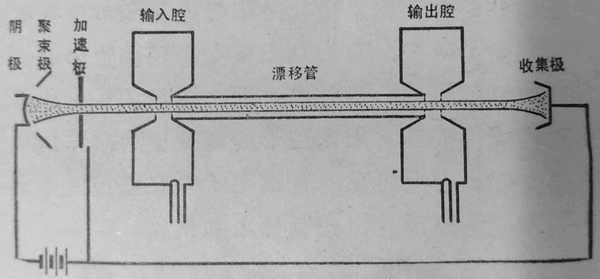
\includegraphics[width=0.9\linewidth]{figure/ch1-1}
	\caption{双腔速调管示意图}
	\label{ch1-1}
\end{figure}

\begin{enumerate}
	\item 高速电子流胡产生。阴极发射出来的电子,在高达几千伏的阳极电压加速下得到了足够大的速度,因而具备了足够大的动能。与普通电子管中的阳极不同,速调管中的阳极是中心开孔的,他只对电子进行加速而不截获电子。这里阴极、聚束极和阳极组成了一个小部件,叫做电子枪。从电子枪中射出的电子流是一个高速的均匀电子流,下一步就将对它进行速度调制了。显而易见,高速粒子流的动能是直流电源给它的。
	\item 对高速电子流进行密度调制。这个过程是在输入谐振腔和漂移管中完成的。输入交变信号在谐振腔的隙缝处产生交变电场,当高速电子流穿过输入腔隙缝时,交变电场就要对它产生作用,使它的速度受到调制。漂移管实际上就是一根中空的金属圆管,它屏蔽了外界的一切电磁场,为电子流制造了一个无场空间,于是电子流就在里面做惯性运动,逐渐群聚,最后变成和输入信号波形相同的密度调制电子流。这个过程也就是速度调制方法的实现过程。
	\item 密度调制电子流(即群聚电子流)与输出谐振腔隙缝处的交变电场相互作用并把自己的能量交给高频场(以后,我们习惯把微波交变电磁场叫作高频场或微波信号),使它得到放大,于是,在输出腔就可以得到放大了的微波信号。
	
	为什么群聚电子流与高频场相互作用的结果是前者把能量交给后者使后者增强而不是相反呢?分析表明,当群聚电子流穿过输出腔隙缝时,大部分电子是在减速高频场瞬间穿过的,只有小部分电子是在加速高频场瞬间穿过的。我们知道,电子在加速电场中运动时将从电场中得到能量,变成自己附加的动能,因而速度加快,而电场的能量就要减小,电场减弱;电子在减速电场中运动时,将把自己的部分动能交给电场,使电场能量增大,电场增强,而电子则由于失去了部分动能,因而速度减小。因此大部分电子流在减速高频场瞬间穿过输出腔隙缝的结果就将使群聚电子流有净的能量交给高频场,使它得到增强,最后得到放大的高频信号。这个过程是电子流把自己从直流电源中得来的部分动能交给高频电场使之增强的过程,因此是双腔速调管中最本质的过程。	
	\item 收集工作完毕的电子流。这个任务由收集极来完成,从输出腔隙缝穿出的电子流带着剩余的动能打上收集极并全部变为热能。
\end{enumerate}

从上面所分析的四个物理过程中,我们可以得出一个重要的结论:双腔速调管是借助于交变电子流来实现直流电场和高频电场之间的能量转换,从而使高频信号得到放大的一种器件。实际上,这个结论对于一切用于放大的电子管都是适合的。下面,我们将看到,在行波管中也存在着相同的四个物理过程(但实现这四个物理过程的方法有所不同),双腔速调管中的群聚和能量交换这两个概念同样也是行波管中最基本的概念,因此,上面的分析对于我们了解行波管的工作原理是有帮助的。

双腔速调管虽然可以对微波信号进行放大,但是它却不能很好地满足微波通信的要求,其主要原因就是双腔速调管的频带窄。在第二章中,我们将分析双腔速调管频带窄的原因,并由此导出行波管的工作原理。

\chapter{行波管的构造和工作原理}
\section{行波管的构造}
我们来看一只微波通信中常用的中小功率行波管,这类行波管都采用螺旋线来作为它的慢波系统,因此又叫做螺旋线型行波管,图\ref{ch2-1}是它的基本结构图。图\ref{ch2-2}则是其各电极的电源接线图。由图可见,行波管和双腔速调管一样,都有阴极、聚束极、加速极和收集极。不同的地方就在于:我们在行波管中用慢波系统(螺旋线)代替了速调管中的谐振腔和漂移管。这样一来,输能装置也发生了相应的变化。关于行波管中采用慢波系统的原因,我们将在后面讲到。

\begin{figure}[phtb]
	\centering
	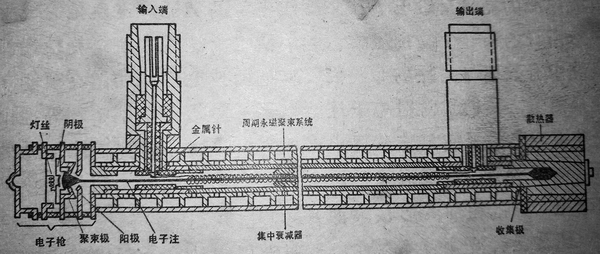
\includegraphics[width=\linewidth]{figure/ch2-1}
	\caption{行波管基本结构示意图}
	\label{ch2-1}
\end{figure}

\begin{figure}[phtb]
	\centering
	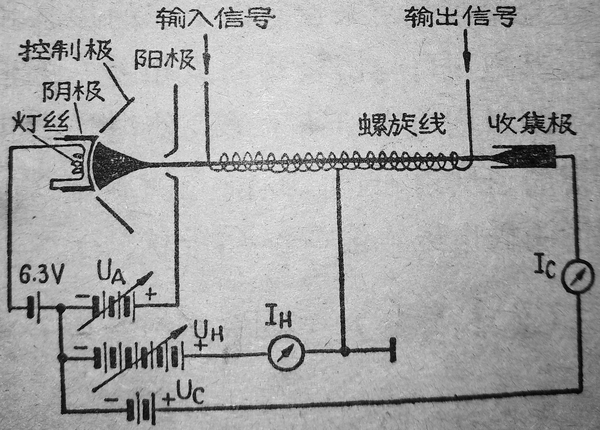
\includegraphics[width=0.65\linewidth]{figure/ch2-2}
	\caption{行波管各极电源接线图}
	\label{ch2-2}
\end{figure}

通常,一只行波管由五部分组成:
\subsection{电子枪}
电子枪通常由阴极、聚束极和加速极(即阳极)组成。它的任务是产生一束具有一定能量的高速细束电子流(常叫做电子注或电子束)。从能量关系来看,电子枪所做的工作就是把直流电源的能量交给电子注,变成电子的动能,也就是完成上一章所说的第一个物理过程。为了使电子注能够在螺旋线慢波系统中有效的与高频场(我们习惯把微波电磁场叫做高频场)交换能量,我们常常对电子注的直径、形状、电流密度等提出一些要求。为了满足这些要求,就需要在电子枪里面增加一些新的电极,例如聚束极就是。电子枪中各个电极的形状和电压,对于电子注的粗细、形状等都有影响。

阴极是行波管的“心脏”,通常用镍的合金制成,发射面做成凹球面状,其表面涂敷一层发射电子的活性物质。

聚束极是用来控制电子注的形状和粗细的,常做成漏斗状,其电压可与阴极相同或相差(低于或高于)几十伏。

阳极则用来加速电子,使电子离开阴极穿过阳极小孔后以一定的速度射入慢波系统(螺旋线)。对中小功率行波管来说,阳极电压一般是2—3千伏。
\subsection{信号输入、输出耦合装置(或输能装置)}
常见的有同轴和波导两种形式,图2-1所示的耦合装置为同轴形式,其内导体与金属针上端接触,金属针下端,则在管内与螺旋线的端部焊牢。同轴接头的外导体与金属管壳相接触。需要放大的高频信号(我们习惯把微波信号叫做高频信号,因而把行波管中与微波信号有关的部分称为高频部分或高频结构。通常我们所说的高频结构,主要就是指慢波系统)由输入装置送入管内,放大后的信号则由输出装置输出。
\subsection{螺旋线慢波系统}
它被用来降低高频场沿管轴的传播速度,使之与电子注的速度相近,以便与电子注进行充分的能量交换,完成把电子的动能转换成高频场能量这一物理过程(详见第三章)。
\subsection{收集极和散热器}
在慢波系统中完成了能量转换任务的电子注穿出螺旋线后被收集极所收集。由于电子注的速度很高,因此收集的热损耗很大,为防止收集极温度过高而损坏行波管,通常在收集外面装有散热器,使能量有效地散出去(详见第八章)。
\subsection{磁聚束系统(磁聚焦系统)}
螺旋线的内径通常只有2—3毫米,电子注的直径就更小,在这样细的电子注内,电子之间的相互排斥力(即所谓空间电荷斥力)很大。因此,要使电子注顺利地穿过长达一、二百毫米以上的螺旋线是十分困难的。为了克服这个困难,我们常常采用外加轴向磁场的办法来限制电子注的向外发散,使他能保持一定的粗细,顺利地穿过螺旋线。这个轴向磁场系统便称为磁聚束系统,它也是行波管中很重要的一部分(详见第七章)。

以上介绍的是行波管必须具备的五个基本组成部分,下面让我们看看行波管是怎样放大微波信号的。
\section{行波管放大的基本原理}
\subsection{双腔速调管的频带为什么那么窄?}
双腔速调管的频带之所以比较窄,其根源就在那个“腔”上。我们知道,谐振腔就是微波频率下的振荡回路,只有谐振频率附近的信号,才能够在谐振腔内建立起高频电场,而非谐振频率(离谐振频率较远)的信号就不能在谐振腔内建立起高频电场。因此,当非谐振频率的信号输入到双腔速调管内时,就不能在谐振腔隙缝处,建立起高频电场,因而不能对电子注进行速度调制,当然密度调制也就无从谈起了。可见正是谐振腔这个窄频带元件限制了双腔速调管的工作频带。因此,为了增宽工作频带,就不能采用谐振腔这样的元件。不过在取消谐振腔之前,我们应该搞清楚谐振腔在双腔速调管中所起的作用、它有哪些特点等,这将有助于我们寻找新的能量作用元件。

在双腔速调管中,谐振腔是电子与高频电场进行能量相互作用的场所。由于谐振腔内的高频电场高度集中在栅网隙缝处,那儿的高频电场就特别强,因此,当交变电子流穿过隙缝时,虽然时间非常短,但是它们之间的相互作用是十分强烈的。于是,我们便能在输出腔得到很强的输出信号,达到放大微波信号的目的。可见,谐振腔的特点是:电场集中,与电子流相互作用强烈,但作用时间很短。谐振腔的这个特点是与他是一个驻波型元件分不开的。我们知道,驻波型元件的能量都比较集中,它占有的空间比较小,但频带都比较窄。

看来为了展宽频带,我们不能再用驻波型元件了。于是,人们提出了一个新的想法——采用行波型元件,具体说来就是传输线。传输线在匹配良好的条件下,它的频带是比较宽的。但是,在传输线中,能量是沿传输线不断向前传播的,不像谐振腔隙缝中那样集中,因而与电子流的相互作用也就比较弱。怎样来克服这个缺点呢?我们采取了“因势利导”的办法:既然高频电磁场要沿着传输线不断地向前传播,那么我们能不能让电子流也跟着它一起向前走,使它们之间一边前进一边不断的相互作用呢?这个办法实际上就是用增加相互作用时间(因而必然增加了相互作用距离)的办法,也就是积少成多的办法来实现电子流与高频电场之间较大的能量交换,达到和驻波型元件同样的效果。

上面这个设想实际上就是行波管的一个雏形,行波管就是因其电子流是与行波高频场相互作用而得名的。当然要实现上面的设想,还需要解决一系列的问题,例如:采用什么样结构的传输线?如何使电子流与高频场一起前进?高频信号如何送入传输线中?又如何从传输线中取出?等等。
\subsection{同步}
和双腔速调管不同,在行波管中我们采用的是电子流与高频电场持续相互作用的办法。而这里的高频电场是沿着传输线不断地向前传播的,也就是是一个行波高频场。因此,为了使它们之间能够持续的相互作用,就要求电子流的移动速度与行波高频场的传播速度相同。我们把这个现象称之为“同步”\footnote{下面我们将讲到,所谓“同步”,并不是电子速度与高频场传播速度完全相等,而是电子速度比高频场传播速度要稍大一些。不过,这并不影响我们这里的讨论。},它是行波管中特有的,并且是十分重要的一个特性。

怎样实现电子流与行波高频场之间的“同步”呢?我们首先来看一看它们各自的速度有多大。

我们知道电磁波在真空中是以光速传播的(光速c等于3×十的八次方米每秒)。而电子的运动速度则由其加速电压来决定,例如加速电压为3000伏时,电子的速度\footnote{电子的速度$ v_0 $可根据下式算得:\[v_0 = \sqrt{\frac{2e}{m}U_0} = 5.93\times10^5\sqrt{U_0}\textrm{(m/s)} \] 加速电压$ U_0 $的单位为伏}约为$ 3.3\times10^7m/s $。可见,这时电子的速度,大体上只有光速的十分之一。

为了实现“同步”,我们可以采取两个办法。第一个办法是使电子的速度加大十倍;第二个办法是使电磁波的传播速度减小十倍。很明显第一个办法是不可取的,因为电子的速度是与其加速电压的平方根成正比的,为了使电子的速度增大十倍,加速电压就要增大一百倍!这么高的电压无论在产生、维持和使用等方面,都会出现一系列极难解决的问题。那么第二个办法行不行呢?用什么办法才能使电磁波在传输线中的传播速度减慢呢?下面这个例子给了我们很大的启发。假定有一辆汽车沿着螺旋形的盘山公路向山顶驶去,如果我们按照海拔高度(即山下到山顶的垂直距离)来计算汽车的速度的话,那么这个速度就是汽车的垂直上升速度,它肯定要比汽车的实际行驶速度小。因为汽车沿着盘山公路走完一圈螺旋时,其垂直高度才上升了一个螺距。同样道理,如果让电磁波沿螺旋形的金属导丝向前传播,那么它沿螺旋线轴线方向的传播速度也会减慢。因此,就有可能实现电子流和电磁波之间的“同步”。可见,第二个办法是可行的。我们把凡是能够使电磁波传播速度减慢的传输线统称为慢波线(或慢波系统)。因此为了实现同步,就需要采用这种特殊的传输线——慢波线。中小功率行波管中最常用的慢波线便是上面介绍的螺旋线,他们通常是用钼丝或钼带绕制成的。

电磁波(即高频场)在螺旋线中传播速度的减慢程度可以通过式\ref{eq:ch2.1}进行粗略的计算:
\begin{equation} \label{eq:ch2.1}
	\dfrac{v_p}{c}=\dfrac{p}{2\pi a}
\end{equation}
式中$ v_p $为减慢后的传播速度;$ c $为光速;$ p $为螺旋线的螺距;$ a $为螺旋线的半径。\ref{eq:ch2.1}式的物理意义是很清楚的。因此,我们便可以用改变螺旋线螺距和直径的办法来调节电磁波在螺旋线中的传播速度,为电子流与行波高频场真正达到“同步”创造条件。下面我们将讲到,要使电子流与行波高频场真正达到“同步”,常常还需要采用调节螺旋线电压即改变电子速度的办法。
\subsection{群聚和放大}
我们知道,在双腔速调管中密度调制的交变电子流是通过漂移空间的群聚而得到的,因此叫做群聚电子流。在行波管中,我们也是利用群聚电子流与高频电场的相互作用来放大微波信号的。所不同的是双腔速调管中的电子流群聚过程是在无场(没有外加电场)漂移空间中完成的,而行波管中的电子流则是一边群聚、一边与同步高频场相互作用的。

“同步”与“群聚”是行波管中极为重要的两个概念。关于“同步”,我们已经在前面作了一个简单的介绍。那么,“群聚”又是怎么回事呢?为了便于读者理解下面的内容,我们不妨来复习一下。

所谓群聚,就是指电子流从速度调制转化为密度调制的过程。在这个过程中,本来均匀的电子流发生了汇聚现象,最后变成一群一群或者一团一团的密度调制电子流,“群聚”这个名称就是这样得来的。此密度调制电子流便叫做群聚电子流。

通常,我们采用两种方法来实现“群聚”。一种是排斥场法,它是反射速调管所采用的,另一种就是漂移法,是双腔速调管和行波管采用的方法,因此有必要简单的介绍一下漂移法。

假定密度均匀的高速电子流在A-A面处受到轴向高频电场$ E_z$(其幅度比电子的直流加速电场小很多)的作用[见图\ref{ch2-3}(a)],那么,它的速度中就将出现交变分量$ v=v_0 +v'\sin{wt} $,也就是说得到了一个微小的速度调制。这样,过了A-A面后,电子的快慢就不一样,如果A-A面后是一个无场漂移空间,那么,电子就将以各自的速度作惯性运动。过了一段时间后,情况就发生了变化,速度快的电子跑得远,速度慢的电子跑得近,电子流的密度便渐渐不均匀了。再经过一段时间,这种情况将继续发展下去,于是,出发晚、速度快的电子就可能追上出发早、速度慢的电子,最后,电子流就变成一群群或者一团一团的了,也就是说,得到了密度调制的电子流群聚电子流。

图\ref{ch2-3}是群聚电子流的形成示意图。我们先来看看经过一个调制电场周期后电子的情况(图\ref{ch2-3}(b)),我们把一个周期的时间分成八等分,分别以$t_0$、$ t_1 $、$ t_2 $、$ \cdots $ $ t_8 $表示。并把$ t_0 $时刻进入A-A面的电子叫做0号电子,$ t_1 $时刻进入A-A面的电子叫1号电子$ \cdots $,依次类推。我们假定调制电场$ E_z $的正方向与Z轴的正方向相同,因此,0号电子未受到加速或减速,1号、2号、3号电子都受到加速$ \cdots $。

由图\ref{ch2-3}(b)可以看出,经过一个周期以后,电子的空间分布就变得不均匀了。不过,它们的分布是很有规律的,1号、2号、3号电子都朝前向0号电子靠拢,5号、6号、7号电子则朝后向8号电子靠拢,就像“两极分化”一样。为了进行比较,我们在图\ref{ch2-3}(a)中画出了$ t=t_s $时未调制电子流的空间分布,这是一个均匀分布。
\begin{figure}[phtb]
	\centering
	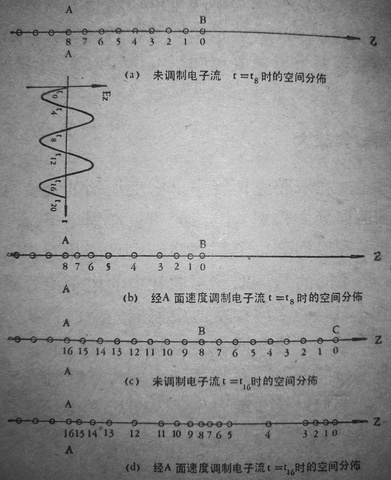
\includegraphics[width=0.8\linewidth]{figure/ch2-3}
	\caption{群聚电子流的形成}
	\label{ch2-3}
\end{figure}

下面,我们来看看经过两个调制电场周期后(即$ t=16 $时)电子的空间分布情况,如图\ref{ch2-3}(d)所示。由图可见,第一个周期内进入A-A面的那些电子,“两极分化”的程度变得更为严重,空间分布更加不均匀。不难想象,如果电子在漂移空间的这种惯性运动继续进行下去,那么,“两级分化”现象就会越来越严重,最后电子流变成一群一群或者一团一团的了。

从图\ref{ch2-3}我们可以看到,电子流中的电子是分别向0号、8号、16号$ \cdots $等电子靠拢的,这些电子就叫做“群聚中心”,这些电子有一个共同的特点:它们都是当调制电场$ E_z $由正半周变为负半周穿过零点的那些时刻进入A-A面的。由图可见,群聚电子流的密度将在这些“群聚中心”附近达到最大,因此,群聚电子流的密度调制频率是和调制电场$ E_z $的频率一致的。

现在,我们再回到行波管来。我们知道,在行波管中,始终有一个同步高频场随着电子流一起前进,那么,读者要问:同步高频场的存在会对电子流的群聚产生什么影响呢?是加强了群聚还是破坏了群聚?反过来,群聚电子流又是如何作用于同步高频场的呢?是把自己的能量交给高频场还是从高频场中得到能量?对于这两个问题的简要回答是:由于电子流与高频场是同步前进的,因此它们之间就可以持续地相互作用,互相得到加强:在同步高频电场的作用下,电子流的群聚不断得到加强;反过来,群聚电子流又不断地把自己的能量交给高频电场,使它增强。它们共同增长的结果就是在输出端处得到了比输入信号强得多的信号,这样,输入信号便得到了放大,这就是行波管的放大原理。我们把行波管内电子流密度和高频电场共同增长的情况形象地画在图\ref{ch2-4}中。
\begin{figure}[htbp]
	\centering
	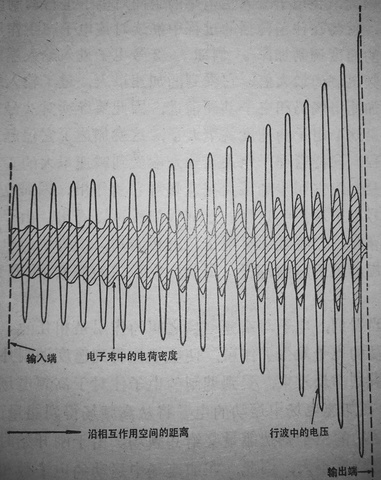
\includegraphics[width=0.7\linewidth]{figure/ch2-4}
	\caption{信号电压和群聚沿行波管相互作用而增长的情况}
	\label{ch2-4}
\end{figure}

下面,我们来比较详细地分析一下行波管内电子流与行波高频场相互作用的情况,以回答前面所提出的问题。

当均匀电子注进入螺旋线时,输入端处的高频电场就要对电子注进行速度调制。由于输入端的高频电场比较弱,因此电子注受到的速度调制是不大的。这些具有初步速度调制的电子注在继续向前运动的过程中将会受到螺旋线上高频电场的作用。图\ref{ch2-5}就表示了高频电场对电子流群聚的作用。图中画出了有同步高频电场存在时某两个时刻电子的空间分布图。和前面一样,我们规定$ E_z $的正方向与$ Z $轴的正方向相同,因此,对电子来说,$ E_z $为负时是加速场,$ E_z $为正时是减速场。在同步情况下,在输入端对电子进行初步速度调制的高频电场将与被调制的电子以相同的速度向前移动,它们之间处于相对静止状态。因此,在电子进入输入端的瞬间对电子进行调制的那个高频场,就将在往前传播的过程中继续对该电子产生作用,使得电子的速度调制加深。例如:2号电子进入输入端时正好碰上高频电场的最大值,它受到的加速最大,过了输入端后此最大加速电场仍和电子共同前进,因此要继续对2号电子加速,结果这个电子的速度就更大了,这就加速了它追赶0号电子的过程。同样道理,原来在输入端受到减速最大的6号电子将继续受到跟它同步的最大减速场对它的作用,因而也加速了它向8号电子靠拢的过程。这样我们就可以看出,由于同步高频场的存在,它将继续对电子注进行调制,使得快的电子越跑越快,慢的电子越跑越慢,因此,电子注的群聚便得到了加强。
\begin{figure}[phtb]
	\centering
	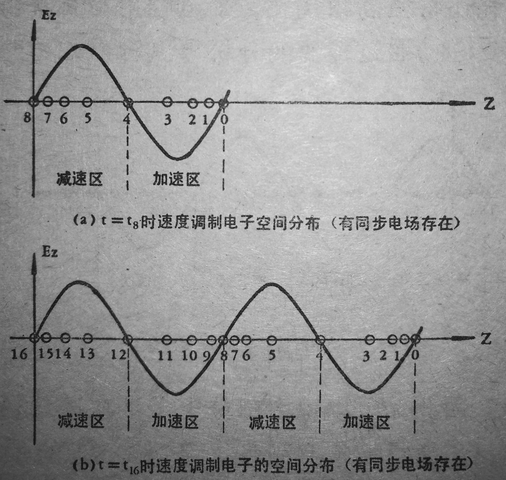
\includegraphics[width=0.65\linewidth]{figure/ch2-5}
	\caption{同步高频电场加强了电子流的群聚}
	\label{ch2-5}
\end{figure}

应当看到,电子与高频电场之间的作用是相互的。高频电场对运动的电子发生了作用,使电子注得到速度调制并逐渐变为密度调制;反过来,受到调制的电子注对于高频电场也要发生作用,在加速电场中运动的电子将从高频场得到能量,而在减速场中运动的电子则把能量交给高频场。由于刚开始时,电子注的群聚程度不大,因此,在加速场中运动的电子数和在减速场中运动的电子数基本上是相等的,总的效果是电子注和高颜场之间没有什么净能量交换。但是,当电子注和同步高频继续向前移动时,情况就不同了。从图\ref{ch2-5}(b)中我们可以看到,电子是向0号、8号、16号这样一些“群聚中心”电子掌拢的。因此,我们只要看看群聚中心的电子是在哪种性质的高频场中运动就可以知道总的能量交换是哪一方面占优势了。如前所述,群聚中心都是高频电场从减速场转为加速场穿过零点这一瞬间进入输入端的那些电子。那么,这些电子将在什么性质的高频场中运动呢?下面,我们来讨论几种情况:
\begin{enumerate}
	\item 假定电子注速度的直流分量是$ v_0 $,高频场的轴向传播速度为$ v_p $,如果两者完全相等,那么群聚中心就始终在零场中运动,群聚的电子群中有一半电子在加速场中运动,另一半在减速场中运动。因此,虽然电子注已经群聚,但由于群聚中心在零场中运动,总的效果,电子注和高频场之间仍然没有什么净能量交换。
	\item 如果电子的速度比高频场的传播速度略慢(即$ v_0 \leq v_p $),从图\ref{ch2-6}可以清楚地看出,群聚中心将落入加速场中,也就是说大部分电子将在加速场中运动,从高频场中吸收能量。总的效果是高频场把能量交给电子注,它本身不但得不到放大,反而迅速地衰减下来。
	\item 当电子速度和高频场传播速度相差很大(即$ v_0\gg v_p $或$ v_0 \ll v_p $)时,进入螺旋线的电子注一会儿受到加速场的作用一会儿受到减速场的作用,因而不可能得到有效的群聚,也就不能与高频场发生有效的能量交换。相反,由于螺旋线本身的损耗还将使高频场在传播过程中不断减弱。
	\item 通过前面的分析可以看出,如果要让群聚中心的电子在减速场中运动,就需要使电子注速度$ v_0 $比高频场的轴向传播速度$ v_p $稍快一些。这时的情况就象图\ref{ch2-7}所画的那样,由于群聚群聚中心已经落入减速场中,因此,可以说大部分电子是在减速场中运动的,它们将把自己的能量交给高频场。于是,总的看来,电子就有净能量交给高频场,使高频场增强。由于电子注和高频场始终是同步前进的,因此,这种能量交换是持续不断的。在电子注向前流动的过程中,螺旋线上的高频场不断对它作用,使得它的群聚不断加强;同时,加强了的群聚电子注又不断地把能量交给高频场,使得高频场不断地得到增强。最终,高频场就能得到可观的放大。我们把这个过程形象地用图\ref{ch2-8}表示出来。
\end{enumerate}

通过上面的讨论,我们可以看到:行波管是一种利用电子注与行波高频场之间持续的能量交换作用来放大微波信号的电子器件。由于螺旋线的频带很宽,因此,螺旋线型行波管的工作频带也很宽,这是它的一个很大的优点。行波管的另一个优点是增益高,这是因为在同步条件下,电子注与高频场能够持续地有效地发生能量交换的缘故。

\begin{figure}[phtb]
	\centering
	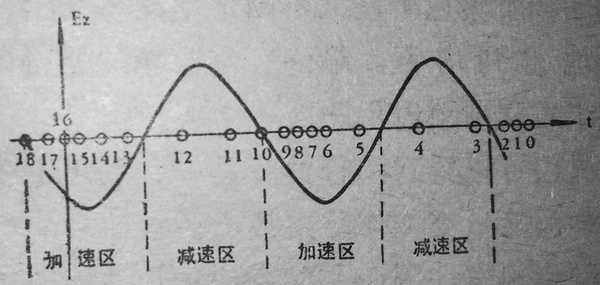
\includegraphics[width=0.6\linewidth]{figure/ch2-6}
	\caption{$ v_0 \leq v_p $时群聚中心落入加速场中}
	\label{ch2-6}
\end{figure}

\begin{figure}[phtb]
	\centering
	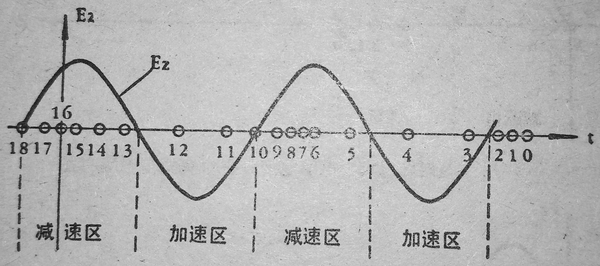
\includegraphics[width=0.6\linewidth]{figure/ch2-7}
	\caption{$ v_0 \geq v_p $时群聚中心落入减速场中}
	\label{ch2-7}
\end{figure}
\begin{figure}[phtb]
	\centering
	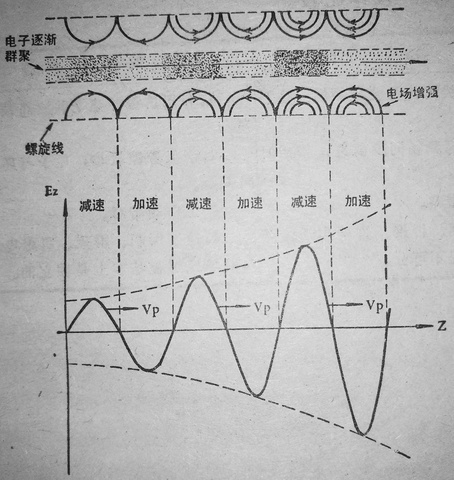
\includegraphics[width=0.65\linewidth]{figure/ch2-8}
	\caption{群聚电子流的形成}
	\label{ch2-8}
\end{figure}
从前面的分析中我们知道,所谓同步就是要使电子注的速度略大于高频场的传播速度,即$ v_0 \geq v_p $。这就是说,我们最初所建立的同步概念(即$ v_0 = v_p $)应当作一些修改。因为正如前面所分析的,当$ v_0 = v_p $时,交变电子流与高频电场之间将没有净能量交换。

在实际的行波管中,螺旋线的尺寸已经通过设计计算确定,也就是说,$ v_p $已经定了。那么,怎样使电子流和行波高频场达到“同步”呢?我们知道,电子的速度可以很方便地通过调节螺旋线电压来改变。因此,只要调节螺旋线电压$ U_H $便可以达到$ v_0 \geq v_p $的同步状态,此时,交变电子流能够最有效地把能量交给高频电场,使行波管的输出功率最大。可见,同步状态是与最大的输出功率相对应的,我们把此时的螺旋线电压叫做同步电压。通常,为了得到尽可能大的输出功率,人们总是把螺旋线电压调节到同步电压工作。

最后,让我们把行波管和双腔速调管的工作特点归纳一下,列成表\ref{tab:ch2-1},以作比较。

\begin{table} 
	\caption{行波管和双腔速调管的比较}\label{tab:ch2-1}
	\begin{tabular}{p{6cm}p{6cm}}
		\toprule
		\centering 行波管          &  \hspace{6em}双腔速调管    \\ \midrule
		\begin{enumerate}
			\item 用慢波线传输行波高频场,电场较弱。
			\item 电子与高频场同步前进,作用时时间长。
			\item 工作频带宽。
			\item 速度调制、群聚、群聚电子流激励高频场三过程不可分。
		\end{enumerate}	    & \begin{enumerate}
			\item 利用谐振腔建立驻波高频场,电场强。  
			\item 谐振腔隙缝小,电子与高频场作用间短。
			\item 工作频带窄。 
			\item 速度调制、群聚、群聚电子流激励高频场三过程基本上是独立的。
		\end{enumerate}	  \\ \bottomrule
	\end{tabular}
\end{table}
 


\chapter{螺旋线}
慢波系统是行波管的主要部件之一,它是管内传播高频电磁波的一种特殊传输线。按照在行波管中所起的作用,我们对慢波线提出了以下三个基本要求:一是能使高频电磁波的传播速度减慢,以便与电子流“同步”,进行充分的能量交换;二是要求慢电磁波的传播速度随频率的变化尽量小,这样,当不同频率的电磁波进入该慢波线时就都能与电子流“同步”,因而都能得到放大,行波管的频带就能做得很宽。讲到这里,读者也许要问:在第二章里不是说过传输线的频带是很宽吗?这里为什么又作为一条基本要求提出来呢?这是因为慢波线一般都不是均匀的传输线,我们知道,均匀传输线(如同轴电缆)的频带是非常宽的,而非均匀传输线的频带就要窄得多,非均匀传输线的频带宽度是与它们的不均匀程度有密切的关系的,不同的慢波线,由于其结构上的不同就会带来频带宽度的不同。因此,我们在设计慢波线的时候,很重要的一点就是要算出它的频带宽度是否能满足我们的要求。对于慢波线的第三个基本要求是希望在慢波线中电子注通过的地方能够建立起较强的轴向电场,这样,电子与高频电场之间才能产生有效的能量交换。

上一章中提到的螺旋线是一种能够较全面地满足上面三个基本要求的慢波线。特别是由于它具备了频带宽这样一条突出的优点,加上其结构简单、容易制作,所以中小功率行波管中几乎毫无例外地都采用螺旋线来作为它们的慢波系统。本章将对螺旋线的主要特效及若干实际问题作一简略介绍。
\section{螺旋线是怎样使电磁波速度变慢的?}
我们来看看图\ref{ch3-1}所示的一根用细金属丝绕成的螺旋线假定它的轴线与坐标轴$ Z $轴重合,平均直径等于$ 2a $,螺距等于$ p $,螺旋角(螺旋线上任意一点的切线与过该点所作$ Z $轴垂直平面之间的夹角称为螺旋角)等于$ \psi $。当电磁波以光速$ c $从螺旋线上的某点$ A $沿细金属丝传播到另一点$ B $时,如果$ B $点正好是沿金属丝绕行一圈到达的那个点,那么,电磁波沿金属丝所传播的距离可由图\ref{ch3-1}右边所示的一圈螺旋线的展开图上求得,它等于$\frac{2\pi a}{\cos \psi} $。但如果我们来观察同一时间内电磁波沿$ Z $轴的传播距离的话,它只前进了一个螺距$ p $。因此,电磁波沿$ Z $轴的传播速度$ v_p $与光速$ c $的比值等于:
\begin{equation}
	\frac{v_p}{c} = \frac{p}{\frac{2\pi a}{\cos \psi}} = \frac{p}{2\pi a}\cdot \cos\psi
\end{equation}
它反映了电磁波沿$ Z $轴的传播速度比光速减慢的程度,叫做螺旋线的“慢波比”。如果知道了电子注的运动速度$ v_0 $,那么就可以适当选择螺旋线的几何尺寸,使得$ v_p \approx v_0 $,即实现电磁波与电子注的“同步”。如前所述,在行波管实际工作时,为了达到真正的“同步”,通常还需要用改变螺旋线电压的办法来调节$ v_0 $,也就是进行“细调”。
\begin{figure}[phtb]
	\centering
	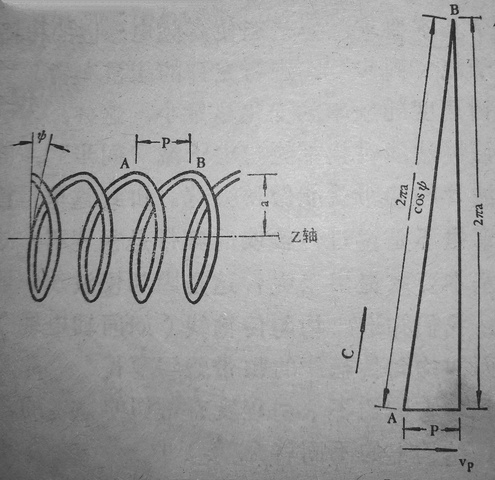
\includegraphics[width=0.65\linewidth]{figure/ch3-1}
	\caption{螺旋线的螺距、螺旋角和半径:$ \frac{v_p}{c} = \frac{p}{2\pi a} \cos \psi$}
	\label{ch3-1}
\end{figure}

上面的分析方法虽然便于直观地理解螺旋线中电磁波传播速度变慢的工作原理,但是,应该指出,这种分析是很粗略的。因此,它不能十分准确地反映实际情况。比如,由它似乎可以得出“慢电磁波的传播速度不随频率而变化”[因为式\ref{ch3-1}中不包含频率$ f $这样的错误结论。实践证明,对一个结构一定的螺旋线来说,虽然慢电磁波的传播速度在一定的频率范围内变化较小,但毕竟还是有变化的,这种变化对于行波管的工作是有影响的。因此,为了准确地设计螺旋线的结构,保证行波管的宽频带运用,就必须进一步研究慢电磁波的传播速度与频率之间的关系,即“色散特性”。


\section{色散特性}
慢电磁波的传播速度随频率而变化的情况,通常都用慢波系统的色散特性来表示。“色散”原是指光学中的一个物理现象。我们知道,光也是一种电磁波,只是它的频率要比微波高得多罢了。光因其频率的不同而呈现各种颜色,而白光则是由多种频率的单色光混合而成的。不同颜色的光在真空中传播时速度都是相同的,但是在介质(例如玻璃等)中传播时,它们的速度就随频率而不同了。因此,如果让不同颜色的光以同一个方向从空气中斜入射到玻璃介质中去,那么,由于折射角将随频率而变化,它们在玻璃中的传播方向就各不相同了。我们可以做一个实验来证实这个现象:让一束白光从空气中入射到玻璃棱镜中去,在玻璃棱镜的后面放置一个白色的屏幕,那么,白光中的各种单色光就将以不同的折射角从玻璃棱镜中射到白色屏幕上,于是,在白色屏幕上我们就可以看到依次排列的红、橙、黄、绿、青、兰、紫等各种颜色,这种现象便称为色散”。可见,色散的本质就是光在介质中的传播速度随频率而变化的特性。我们在描述慢波线中慢电磁波的传播速度随频率而变化的特性时,也采用了这个名称。

螺旋线的色散特性可以通过理论分析和实验测量两种途径得到。图\ref{ch3-2}所表示的螺旋线色散特性,就是在对实际螺旋线作了一定简化假设的条件下,用电磁场理论对电磁波沿螺旋线的传播规律进行数学分析后得出来的。图中纵坐标为$ \frac{v_p}{c} $,因为光速$ c $为常数,所以纵坐标的值是与$ v_p $正比的。横坐标为$ ka $其中$ a $是螺旋线的平均半径,对于结构已经确定的螺旋线来说,$ a $是一个常数。$ k=\frac{2\pi f}{c} $是电磁波在自由空间传播时的相位传播常数,它的物理意义将在后面介绍。由上可见,横坐标$ ka $是与频率$ f $成正比的。因此,图\ref{ch3-2}就表示了$ v_p $和$ f $的关系,也就是色散特性。
\begin{figure}[phtb]
	\centering
	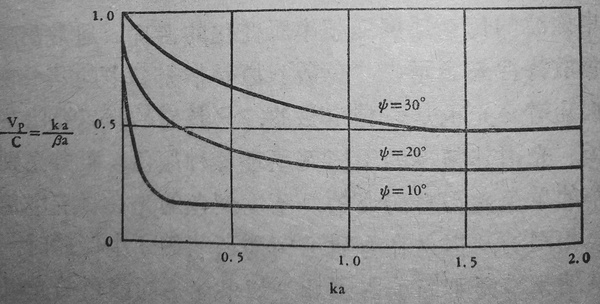
\includegraphics[width=0.65\linewidth]{figure/ch3-2}
	\caption{螺旋线的色散特性曲线}
	\label{ch3-2}
\end{figure}

从图\ref{ch3-2}的曲线中我们可以看到,当频率较高时,$ v_p $基本不变,且只与螺旋角$ \psi $有关。它的数值可以近似用$ \ref{ch3-1} $式算得,在$ \psi $较小的情况下,$ \ref{ch3-1} $式可以写成:
\begin{equation} \label{eq:ch3-2}
	\frac{v_p}{c}= \sin \psi \approx \tan\psi = \frac{p}{2\pi a}
\end{equation}
可以看出,\ref{eq:ch3-2}式是与上一章中的\ref{eq:ch2.1}式一致的。在实际的行波管中,工作频率不能任意提高,因为当频率超过一定范围后将会引起返波振荡(见第\ref{ch5}章),造成行波管工作的不稳定。为了避免返波振荡出现,通常在设计螺旋线时,总是使$ ka < 0.3 $。

我们在设计螺旋线型行波管时,常常是根据一定的原则先确定电子注电压(即螺旋线电压)$ U_0 $,从而也就决定了电子速度$ v_0 $和慢电磁波的传播速度$ v_p $。例如,微波通信设备所用的某中小功率行波管,其$ U_0 $为3千伏,对应的电子速度$ v_0 $约为光速$ c $的十分之一,由此可算得螺旋角约$ 6^\circ $。由图\ref{ch3-2}可见此时的色散特性曲线上有很宽的弱色散区(弱色散区是指$ v_p $随$ f $变化很小的区域,角越小,弱色散区越宽)。因此,尽管把$ ka $限制在0.3以下,由于$ U_0 $较低,$ \psi $较小,我们仍然可以得到很宽的频带。例如,对上例中$ \psi \approx 6 ^\circ $的情况,$ ka $只要大于$ 0.1 $左右,特性就很平了,如果$ a=1.5 $毫米,那么与$ 0.1<ka<0.3 $相对应的频率范围就是$ 3.2<f<9.5 $千兆赫,可见频带是很宽的。

慢波线的色散特性除了能够用$ \frac{v_p}{c}\textasciitilde ka$曲线直观地表示以外,还可以用所谓“$\omega -\beta $”曲线来表示,而且$ \omega-\beta $曲线能够更多地反映出慢波系统的主要特性。为了说明这个曲线,我们先来熟悉一下描述电磁波传播特性的几个基本量。



常数了。由$ \omega \textasciitilde \beta $曲线我们还可以确定慢波线的一些其它传播特性。例如曲线上任意一点的切线斜率就等于波的“群速”$ v_g $(即波的能量传播速度,它和波的相位传播速$ v_p $不同);由曲线的形状可以判断出$ v_g $和$ v_p $的符号是否相同,实际上就是群速和相速的方向是否相同?我们把$ v_g $和$ v_p $,方向相同的波称为“前向波”,而$ v_g $和$ v_p $方向相反的波则称为“返波”。正是由于$ \omega \textasciitilde \beta $曲线能够更多地表示出慢波线的传播特性,所以应用更为广泛。

关于波的群速、前向波与返波等问题,因超出了本书范围,这里不赘述。
\section{耦合阻抗}
耦合阻抗是表征慢波线中轴向高频电场与电子之间能量交换的有效程度的一个参量(用符号$ K_c $表示)。在螺旋线型行波管中,电子注是在螺旋线内沿着它的轴线方向运动的,因此,只有轴向高频电场才能和电子产生能量交换作用。当电磁波沿螺旋线向前传播时,它在电子注流过处(具体说来也就是螺旋线内半径为$ b $的细圆柱体内。$ b $是电子注半径)产生的轴向高频电场越强,那么电子与轴向高频电场的能量交换作用也越强。电子注流过处轴向高频电场的大小与螺旋线的结构有关,螺旋线结构不同时,它的高频场分布就不同,因此为了求出电子注流过处轴向高频电场的大小,就需要找到螺旋线的场分布,图\ref{ch3-5}表示了螺旋线周围的高频场分布。

电子注流过处轴向高频电场的大小还与螺旋线中传播的高频场功率有关。显而易见,送入螺旋线的高频场功率越大,那么它在电子注流过处产生的轴向高频电场也越强。为了便于对不同的螺旋线中电子与场能量交换的有效程度进行比较,我们希望能建立一个统一的衡量标准。首先,在不同的螺旋线中应该送入相同的高频场功率。在相同的高频场功率下,我们再来观察哪一种螺旋线所产生的轴向高频电场大,这样才能比较出哪一种螺旋线的相互作用有效程度强。这实际上就是希望在新导出的用来衡量相互作用有效程度的参量中去掉高频场功率带来的影响。从$\text{压强}= \frac{\text{压力}}{\text{受压面积}} $(即压强等于单位面积所受到的压力)这个公式我们联想到,这个新参量是否可以用送入单位功率所产生的轴向高频电场的大小来表示呢?根据这个想法并类比了低频电路的情况,人们导出了一个新的参量,这就是耦合阻抗$ K_c $。

我们知道,在低频电路中,当我们在谐振频率下往某一谐振回路中送入一定的功率$ P $时,在回路两端所产生的谐振电压振幅$ U $和回路的谐振电阻$ R $有下面的关系:
\begin{equation} \label{eq:ch3-17}
	R = \frac{1}{2}\frac{U^2}{P}
\end{equation}
回路的谐振电阻$ R $越大,那么其两端产生的谐振电压也越大因此$ R $是表征谐振回路特性的一个重要参量。

同样道理,我们把慢波系统的耦合阻抗$ K_c $定义为:
\begin{equation} \label{eq:ch3-18}
	K_c = \frac{1}{2}\frac{\hat{U_z^2}}{P}
\end{equation}
式中$ P $为沿螺旋线传播的高频场总功率。$ \hat{U_z} $为轴向高频电压的振幅,它是从低频电路的关系式\ref{eq:ch3-17}中类比得来的。我们知道,在微波频率下,通常只采用高频电场这个概念,例如我们常常用场强计来测量高频电场的大小,用功率计来测量高频场的功率大小,而从不用伏特计(电压表)来测量微波高频电场。因此,这里所说的轴向高频电压$ \hat{U_z} $是为了和低频电路类比而人为地导出来的一个量,不过,我们可以利用直流电路中电压和电场之间的关系把它和轴向高频电场$ \hat{E_z} $联系起来。我们知道,在均匀直流电场中,$ a $、$ b $两点之间的电压$ U_{ab} $可用电场$ E $和两点之间的距离$ d_{ab} $表示:
\begin{equation} \label{eq:ch3-19}
	U_{ab} = -E\cdot d_{ab}
\end{equation}
负号表示$ U $和$ E $的方向相反。如果不是均匀电场,那么,可以用积分形式表示:
\begin{equation} \label{eq:ch3-20}
	U_{ab} = - \int_{a}^{b}E \cdot \text{d}z
\end{equation}
我们这里的轴向高频电场也不是均匀电场,不过它是一个有规律的非均匀电场,它是按照正弦规律变化的,如在某时刻$ t=0 $观察,则可简化成\ref{eq:ch3-9}式。为了方便起见,我们人为地取$ \tilde{E_Z} $由零变化到最大值这个四分之一周期所对应的轴向距离(即$\frac{1}{4}\lambda_g$)来作为积分区间,于是有:
\begin{equation} \label{eq:ch3-21}
	\hat{U_Z} = -\int_{0}^{\frac{\lambda_g}{4}}\tilde{E_z}\text{d}z=\int_{\frac{\lambda_g}{4}}^{0}\hat{E_z}\sin{\beta z}\text{d}z=\frac{\hat{E_z}}{\beta}
\end{equation}
读者可能要问:积分区间如果取二分之一导波波长行不行呢?回答是完全可以,但必须在任何场合下都这样规定,也就是说应当统一。

将\ref{eq:ch3-21}式代入\ref{eq:ch3-18}式,我们就可以得到耦合阻抗$ K_c $:
\begin{equation} \label{eq:ch3-22}
	K_c = \frac{\hat{E_z^2}}{2\beta^2P}
\end{equation}

由式\ref{eq:ch3-22}可见,流过慢波系统的功率流$ P $一定时,能够建立的轴向场强$ \hat{E_z} $愈强,则慢波系统的耦合阻抗也越大,也就能使场与电子的相互作用越强烈。而一定功率流下所能建立的电场的强弱主要决定于慢波系统的结构和尺寸,所以耦合阻抗$ K_c $的大小就表征了慢波系统在这方面质量的优劣。

知道了螺旋线内轴向电场分布以后,就可以计算出它的耦合阻抗。\ref{eq:ch3-9}式给出了场沿$ Z $轴方向的分布情况。但轴向电场在螺旋线横截面上是怎样分布的呢?图\ref{ch3-6}给出了它的理论分析结果。图中横坐标为螺旋线横截面内从中心出发沿半径方向的距离$ r $,纵坐标为$ r $处轴向电场$ E_z $与螺旋线上($ r=a $处)轴向电场$ E_{za} $的比值。由图可见,轴向电场在螺旋线横截面上不是均匀分布的,而是中心处最弱,半径$ a $处最强。所以计算所得的耦合阻抗$ K_c $沿径向的分布也有相似的曲线形状如图\ref{ch3-7}所示。由于在螺旋线内流过的电子注有一定的半径


\section{特性阻抗}
\section{实际的螺旋线}
\subsection{介质夹持对色散特性的影响}
\subsection{屏蔽筒对色散特性的影响}
\subsection{介质夹持和屏蔽筒对耦合阻抗的影响}
\subsection{导丝尺寸的影响}





\begin{figure}[phtb]
	\centering
	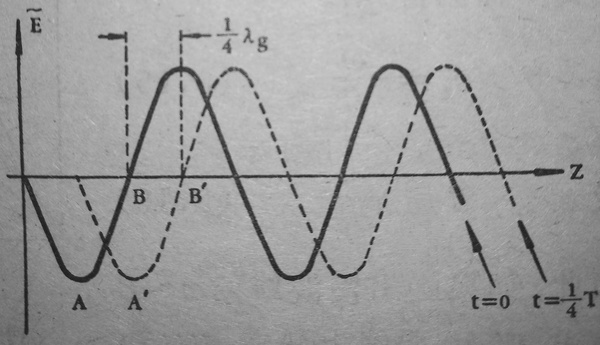
\includegraphics[width=0.65\linewidth]{figure/ch3-3}
	\caption{$ t=0 $和$ t=\frac{1}{4}$时刻,场分量沿$ Z $轴的变化曲线}
	\label{ch3-3}
\end{figure}

\begin{figure}[phtb]
	\centering
	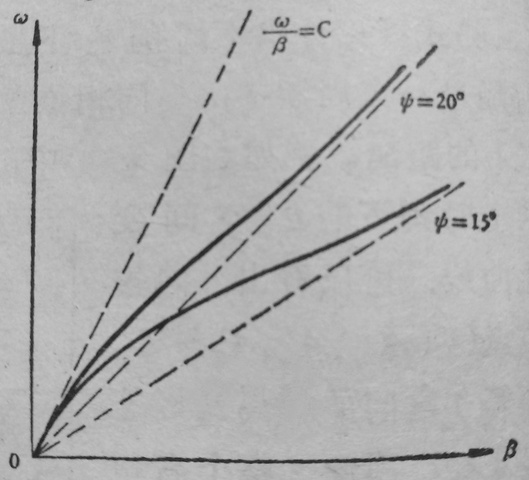
\includegraphics[width=0.65\linewidth]{figure/ch3-4}
	\caption{螺旋线的$ \omega \textasciitilde \beta $曲线}
	\label{ch3-4}
\end{figure}


\begin{figure}[phtb]
	\centering
	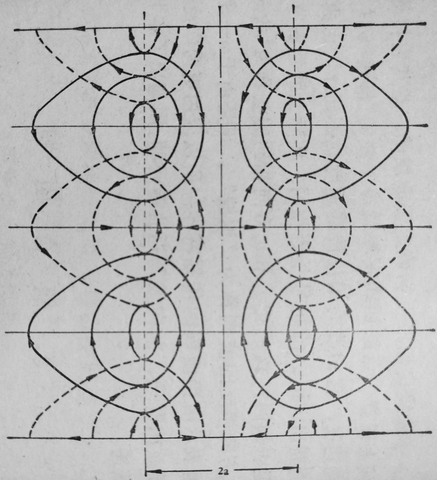
\includegraphics[width=0.65\linewidth]{figure/ch3-5}
	\caption{螺旋线周围电场和磁场分布示意图。实线为电力线,虚线为磁力线。}
	\label{ch3-5}
\end{figure}

\begin{figure}[phtb]
	\centering
	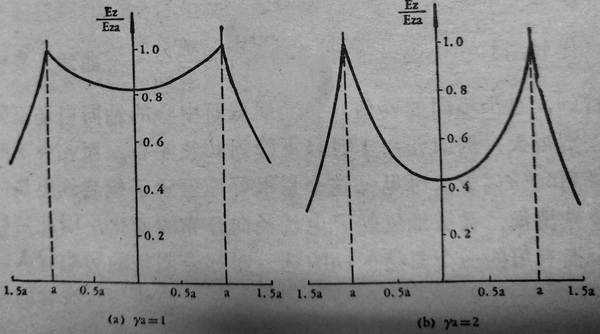
\includegraphics[width=0.65\linewidth]{figure/ch3-6}
	\caption{螺旋线中轴向电场的径向分布示意图}
	\label{ch3-6}
\end{figure}

\begin{figure}[phtb]
	\centering
	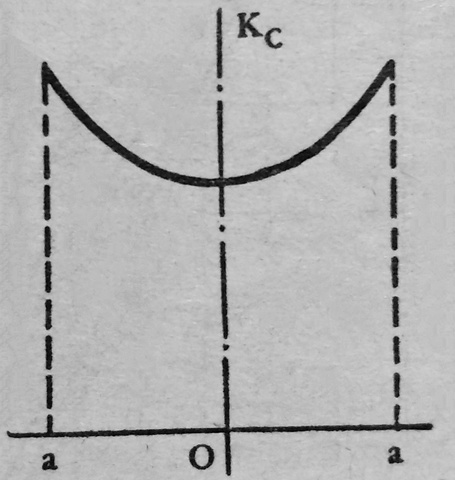
\includegraphics[width=0.65\linewidth]{figure/ch3-7}
	\caption{螺旋线耦合阻抗的径向分布}
	\label{ch3-7}
\end{figure}

\begin{figure}[phtb]
	\centering
	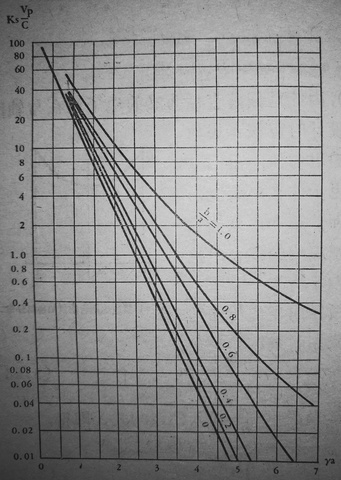
\includegraphics[width=0.65\linewidth]{figure/ch3-8}
	\caption{对于不同的$ \frac{b}{a} $螺旋线耦合阻抗与$ \gamma a $的关系}
	\label{ch3-8}
\end{figure}

\begin{figure}[phtb]
	\centering
	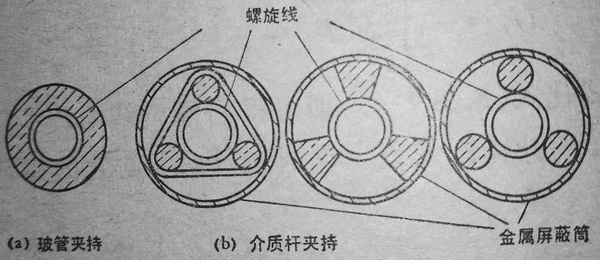
\includegraphics[width=0.65\linewidth]{figure/ch3-9}
	\caption{几种常用的螺旋线加持方法(横截面图)}
	\label{ch3-9}
\end{figure}

\begin{figure}[phtb]
	\centering
	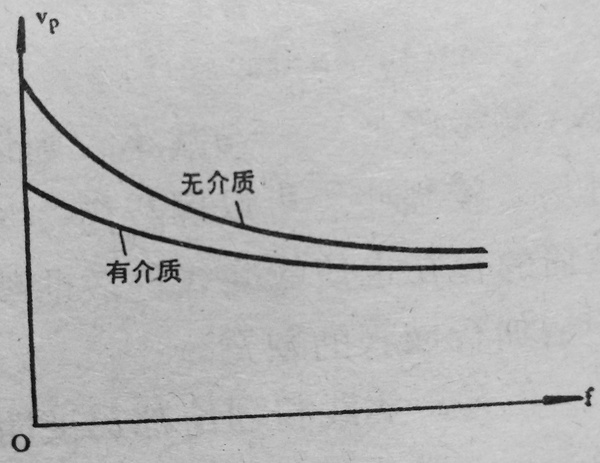
\includegraphics[width=0.65\linewidth]{figure/ch3-10}
	\caption{介质的存在使$ v_p-f $ 曲线变得更平坦}
	\label{ch3-10}
\end{figure}

\begin{figure}[phtb]
	\centering
	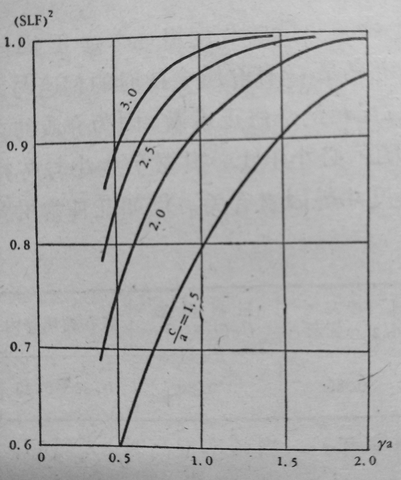
\includegraphics[width=0.65\linewidth]{figure/ch3-11}
	\caption{屏蔽筒加载因子SLF$ ^2 \textasciitilde \gamma a$曲线}
	\label{ch3-11}
\end{figure}
\chapter{行波管的放大能力} \label{ch4}
行波管是一种放大微波信号的器件,因此放大能力是它的主要参数,并且通常用增益来表示。增益($ G $)的意义如下:
\begin{equation} \label{eq:ch4-1}
	G=10\lg\frac{P_\text{出}}{P_\text{入}}(\textrm{dB})
\end{equation}
其中$ P_\textrm{入} $为加到行波管输入端待放大信号的功率,而$ P_\text{出} $是在输出端得到的放大后的信号功率。$ G $的单位是分贝,$ G=10 $分贝相当于放大十倍;20分贝相当于放大100倍;30分贝相当于放大1000倍等等。

微波信号在行波管内所以能被放大,是因为在螺旋线内流动的电子注与外加信号所建立的高频场发生了能量转换的结果。因而行波管放大能力将主要由这两方面的条件及相互作用情况所决定。本章先着重定性讨论这些因素对行波管增益的影响,最后简略介绍一下增益计算的主要问题。
\section{电子注参量对增益的影响}
中小功率行波管中采用的电子注,基本上都是圆形截面的实心电子注。可以用三个参量来表征这种电子注的主要状况即:电子注电流$ I_0 $、电子速度$ v_e $(它是螺旋线电压$ U_0 $所决定)以及电子注截面半径$ b $。下面分别看看这三个因素改变时行波管增益如何随之变化。
\subsection{电子注电流的影响}	
	电子注电流($ I_0 $)越大,则参与同高频场相互作用的电子数目就相应增多。这就是说,有较多的电子受高频场的作用而群聚在减速场里,从而也就有更多的电子将其一部分动能转换为高频场的能量,使信号得到更充分的放大。所以电子注电流$ I_0 $增加对提高增益有利。
\subsection{电子注电压的影响}	
	电压$ U_0 $越高,则电子速度越快,惯性越大,因而在高频场作用下,就比较不容易改变其速度和位置,即不易很快地群聚起来。要使电子迅速群聚起来,就要有较强的高频电场,即需要在行波管输入端送进较强的信号功率($ P_\text{入} $)。否则,因电子注群聚较慢,输出端得到的放大后的信号功率就会减小。由\ref{eq:ch4-1}式可以看出,无论是输入功率$ P_\text{入} $增加,还是输出功率$ P_\text{出} $减小,都直接导致行波管的增益下降。所以,在同样的电子注功率(即:乘积$ U_0I_0 $)下,通常是较大的电流及较低的电压对提高管子增益有利些。	
	
	为了能够同时考虑电子注电流和电压增益的影响,常常使用一个叫“导流系数”的参量($ P_\theta $),它的定义是:
	\begin{equation} \label{eq:ch4-2}
		P_\theta = \frac{I_0}{U_0^{3/2}}
	\end{equation}
	
  由前面的讨论及导流系数的定义可以看出从提高行波管增益的角度考虑,希望电子注导流系数大些。但是,加大电子注导流系数,就要提高对磁聚束系统的要求,增加磁聚束的困难(见第\ref{ch7}章)。这就使电子注导流系数的提高受到一定限制。
	\subsection{电子注直径的影响}	
	我们由图\ref{ch3-6}已经知道,对于螺旋线慢波系统来说,螺旋线横截面内轴向电场的分布特点是:中心处最弱,沿半径方向由轴心往外逐渐增强,在接近导线表面时,轴向场达最大值。可见,如果螺旋线直径($ 2a $)及导波波长$ \lambda_g $一定,则随着电子注直径($ 2b $)的增大(即$ \frac{b}{a} $值增大),与电子注相互作用的平均轴向电场也相应增大,使电子注与高频场的相互作用增强。所以增大电子注直径对提高管子增益是有利的。但是应该指出随着电子注直径增大,电子注更加靠近螺旋线导丝,这就增加了电子被螺旋线截获的危险聚束性能就可能变坏。为了保证必要的聚束状态和聚束稳定性,通常$ \frac{b}{a} $值都在0.6以下。




\section{高频电场对增益的影响}
沿螺旋线传播一定功率的微波信号时,信号在电子注流经的地方所建立的高频电场的强弱及分布状况,直接影响着它与电子注能量交换的有效程度。从第三章关于螺旋线基本特性的介绍中我们知道,耦合阻抗Kc正是表征高频场与电子注相互作用有效程度的基本参量。耦合阻抗越高,则与电子注相互作用的高频电场越强,行波管的增益也就越高。


下面根据图\ref{ch3-8}所列曲线讨论一下影响螺旋线耦合阻抗$ K_c $(也就是影响与电子注相互作用的高频电场)的几个具体因素:
 \subsection{螺旋线直径对增益的影响}
	
	由图\ref{ch3-8}的曲线可以看出,当$ \gamma $及$ \frac{b}{a} $一定时,耦合阻抗$ K_c $





\begin{figure}[phtb]
	\centering
	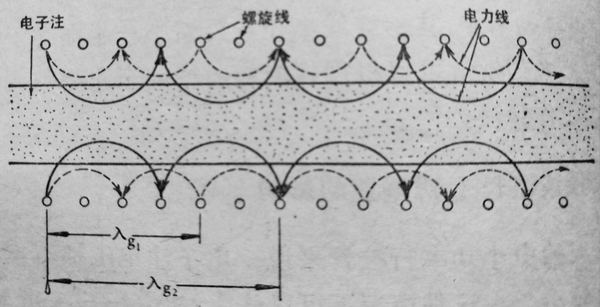
\includegraphics[width=0.65\linewidth]{figure/ch4-1}
	\caption{慢波波长改变时,高频场电力线形状变化示意图}
	\label{ch4-1}
\end{figure}

\begin{figure}[phtb]
	\centering
	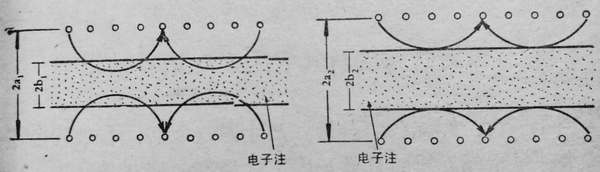
\includegraphics[width=0.65\linewidth]{figure/ch4-2}
	\caption{螺旋线直径增大后,进入电子注的电力线减少}
	\label{ch4-2}
\end{figure}

\begin{figure}[phtb]
	\centering
	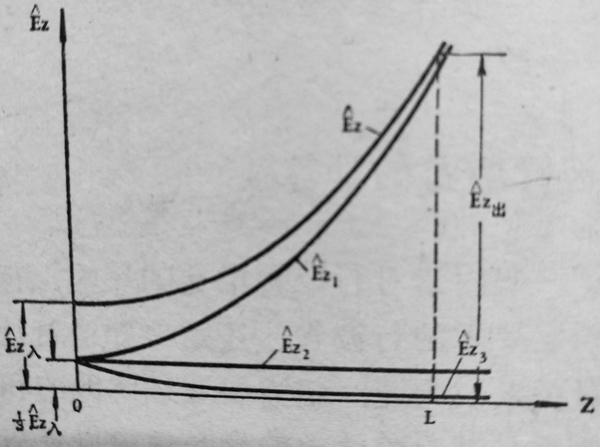
\includegraphics[width=0.65\linewidth]{figure/ch4-3}
	\caption{轴向高频电场沿$ Z $轴变化情况示意图}
	\label{ch4-3}
\end{figure}







\chapter{怎样克服自激振荡}\label{ch5}
\section{自激振荡是怎么回事?}
\section{内部反射引起的自激振荡}
\section{外部反馈引起的自激振荡}
\section{二次电子引起的自激振荡}
\section{怎样判断自激振荡?}







\begin{figure}[phtb]
	\centering
	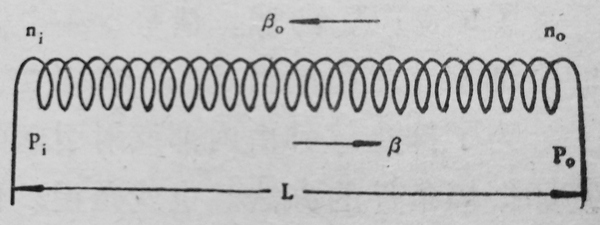
\includegraphics[width=0.65\linewidth]{figure/ch5-1}
	\caption{内部反射引起自激振荡的振幅条件$ G>\frac{L}{n_i n_o} $}
	\label{ch5-1}
\end{figure}

\begin{figure}[phtb]
\centering
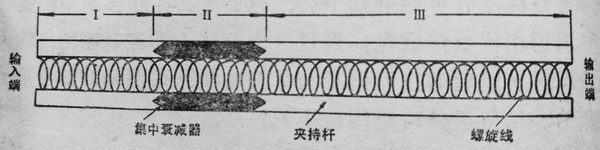
\includegraphics[width=0.65\linewidth]{figure/ch5-2}
\caption{行波管中的集中衰减器}
\label{ch5-2}
\end{figure}

\begin{figure}[phtb]
	\centering
	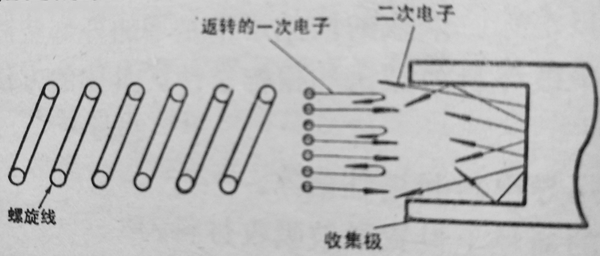
\includegraphics[width=0.65\linewidth]{figure/ch5-3}
	\caption{二次电子和反转的一次电子进入螺旋线}
	\label{ch5-3}
\end{figure}

\begin{figure}[phtb]
	\centering
	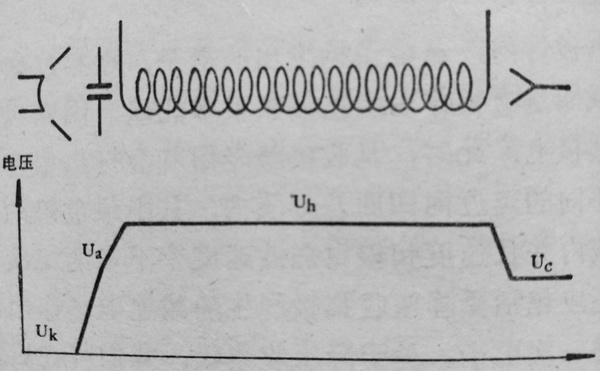
\includegraphics[width=0.65\linewidth]{figure/ch5-4}
	\caption{收集极降压行波管的电位分布}
	\label{ch5-4}
\end{figure}

\begin{figure}[phtb]
	\centering
	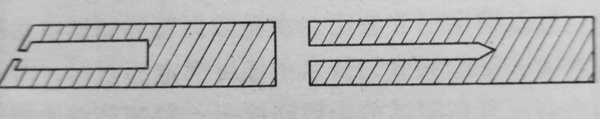
\includegraphics[width=0.65\linewidth]{figure/ch5-5}
	\caption{改进收集极结构}
	\label{ch5-5}
\end{figure}

\begin{figure}[phtb]
	\centering
	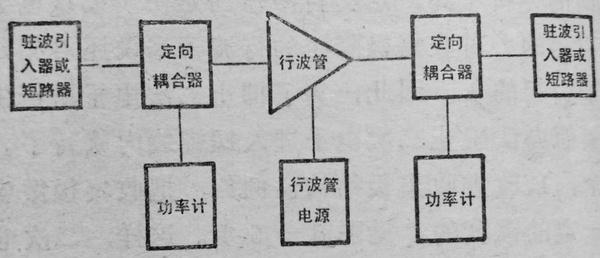
\includegraphics[width=0.65\linewidth]{figure/ch5-6}
	\caption{行波管自激振荡测试方框图}
	\label{ch5-6}
\end{figure}
\chapter{细电子注是怎样得到的?}

行波管是利用电子注与高频电场之间的持续相互作用来实现微波信号放大的一种器件。因此,首先要解决的问题就是如何得到一束符合要求的电子注。实际上,从某种意义上说,行波管的工作过程就是电子注产生、成形、维持和消失的过程。从电子注角度来看,行波管可以分为下面四个区,如图\ref{ch6-1}所示。

\begin{figure}[phtb]
	\centering
	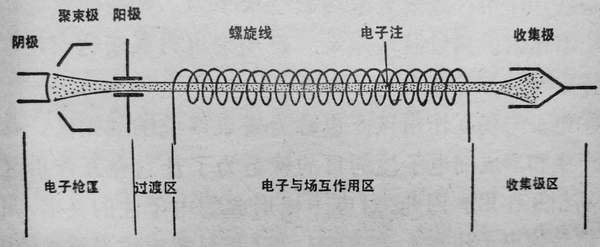
\includegraphics[width=0.65\linewidth]{figure/ch6-1}
	\caption{行波管中的电子注}
	\label{ch6-1}
\end{figure}

\begin{enumerate}
	\item 电子枪区:在此区,电子枪产生电子注并使它基本成形。这个任务是由阴极、聚束极和阳极来完成的。从阴极发射出来的电子在这三个电极产生的静电场和电子注本身空间电荷力的作用下形成一束高速细电子注(可以认为前者将使电子注会聚后者使电子注发散),并从阳极孔射出,这个情况好像子弹从手枪中射出来一样。因此,人们给这种形成和射出电子束的部件起了一个名字,叫做电子枪。	
	
	顺便提一下空间电荷力,它实际上就是电子注内电子与电子之间的相互作用力。我们知道,电子与电子之间存在着互相排斥的作用力,它们之间的距离越近,这种排斥力就越大。因此,当许多电子汇集在一起形成细电子注时,它们之间就会产生较强的排斥力,我们称之为空间电荷力,它将使电子注散开,因而是不利的因素。
	\item 过渡区。这是电子枪区和互作用区之间的中间区域。在电子枪区,作用于电子注的会聚力是静电场产生的,而发散力则是电子注中空间电荷产生的。从阴极出来的电子在这两种力的作用下形成了我们所需要的高速细电子注。在互作用区,作用于电子注的发散力依然是电子注的空间电荷力,但是会聚力却变成了磁场聚束力(详见第\ref{ch7}章)。过渡区的情况介于二者之间,在这里,电子枪电极建立的静电场急剧减小,取而代之的则是从互作用区延续过来的磁场聚束力,而空间电荷发散力则继续起作用。到过渡区末端,磁场聚束力逐渐达到互作用区中那样大小,细电子注也已成形。
	\item 电子与场互作用区,也称为聚束系统的规则区。我们知道,产生和形成细电子注的目的就是为了让它在互作用区中与高频场相互作用。因此,对电子枪形成的电子注的要求,归根到底也就是使电子注在互作用区(细而长的螺旋线慢波系统)中能够很好地同高频场持续相互作用。为此,我们对电子注提出这样三个要求:$ a .$高速:电子注应具有较高的速度,以便具备足够的动能与高频场交换。$ b. $细束:在厘米波段,螺旋线的平均直径一般是2\textasciitilde3毫米,因此要求电子注的直径约在1\textasciitilde2毫米以内。$ c. $层流特性好(关于层流特性,在本章后半部分介绍)。
	
	关于互作用区的情况,我们将在第七章中专门进行分析。
	\item 收集极区。在这个区域内,与高频场作用完毕的电子将被专门的收集极所收集,电子注在此区域内消失。
\end{enumerate}


\section{电子枪的分类}

我们知道,在普通三极管中没有电子枪,这是因为对其电子流的形状和尺寸要求并不严格,只要能得到一定的阳极电流以便在栅阳空间中与交变电场进行能量交换就可以了,它的电子流形状如图\ref{ch6-2}所示。但是,在速调管、行波管以及示波管、显象管等类电子管中,对电子流(这里应称为电子束或电子注)的形状甚至尺寸都有比较严格的要求。怎样得到一束尺寸符合我们要求的规则的电子束呢?我们利用多个电极产生的静电场来使电子束成形,以满足我们的要求。这多个电极便组成了一把电子枪。

\begin{figure}[phtb]
	\centering
	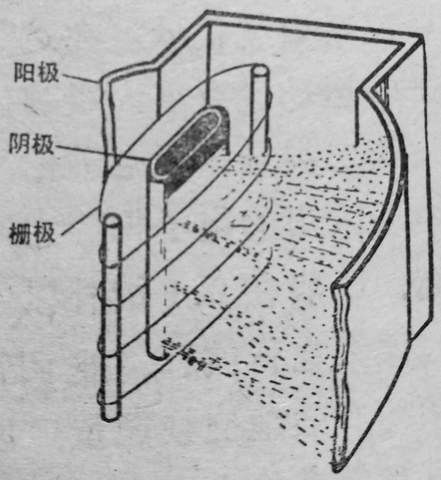
\includegraphics[width=0.3\linewidth]{figure/ch6-2}
	\caption{三极管内电子流示意图}
	\label{ch6-2}
\end{figure}


最简单的电子抢是由三个电极(阴极、聚束极和阳极)所组成的,图\ref{ch6-3}所示的两把电子枪就是这样。随着管子对电子束要求的不断提高,出现了许多种电子枪。但是,我们可以根据电子束的强度把它们分成两大类。由于导流系数很好地表示了电子束的强度,因此,常常用导流系数来区分这两类枪。

第一类是细束电子枪(或弱流电子枪),它产生低强度的电子束。显象管、示波管中采用的就是这类枪。它的特点是导流系数很低(一般在千分之一微朴以下),电子束直径很小(只有0.1\textasciitilde0.5毫米左右,因而称为“细束”)。在这类管子中为了在荧光屏上得到亮度高、直径小的光点,电子束的加速电压都很高(近万伏甚至更高,因为荧光屏的亮度将随电子束动能的增加而增大),而电子束的电流都很小(如显象管的电流约100\textasciitilde1000微安,示波管的电流约10\textasciitilde100微安。由于电流很小因此很便于用偏转电压或偏转线圈来控制它的运动以便在荧光屏上方便地得到和电信号相对应的图象或曲线),因此它的导流系数就很低。在这类低强度的电子束中,空间电荷力对电子的运动没有重大影响,因此可以忽略空间电荷的作用。

第二类是强流电子枪,这就是行波管、速调管等微波电子管中所采用的电子枪。它产生高强度的电子注,其导流系数比较高,一般在0.1微朴以上,有的高达几微朴。这是什么原因呢?原来在行波管、速调管等微波电子管中,为了使电子注和高频均有效地交换能量,以便得到足够大的功率增益,常常希望有足够多的电子参予作用,因而这些管子的电流都比较大一般都在几十毫安以上,有的甚至在几百毫安以上。可见,要比细束枪的电流大得多,故称为强流电子枪。另一方面,为了改善管子的高频性能、提高效率,我们常常希望电子注电压不要太高,对于中小功率行波管来说,通常在1000\textasciitilde3000伏之间。上面两个方面的原因使得强流枪电子注的导流系数比细束枪电子束的导流系数大得多。在强流枪产生的电子注中,电流密度都很大,因此空间电荷力的影响严重,它是使电子注向外发散的最主要原因。可见,导流系数实际上也表征了电子注内空间电荷力的大小。

\section{行波管电子枪的构造}



\subsection{会聚状电子注}



\begin{figure}[phtb]
	\centering
	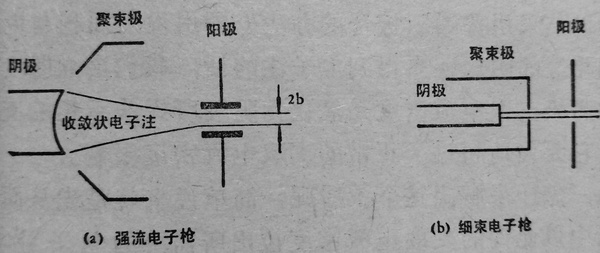
\includegraphics[width=0.65\linewidth]{figure/ch6-3}
	\caption{电子枪结构示意图}
	\label{ch6-3}
\end{figure}

图\ref{ch6-3}(a)是一把行波管电子枪的结构示意图。它是由凹球面状的阴极、漏斗状的聚束极和中心带孔的阳极组成的。我们首先来看看阴极。为什么阴极的面积要比电子注截面面积大很多呢?原来各种阴极都有一定的支取电流密度限制(如氧化物阴极的支取电流密度通常要求在200 mA/cm$ ^2 $以下),如果超过这个限制,就要使阴极的负担过重,因而其寿命将大大缩短。在普通三极管中,通常不会出现阴极支取电流密度超过限制的情况,例如某三极管,其阳极电流为25 mA,阴极面积为0.24 cm$ ^2 $,因此阴极支取电流密度为$ \frac{25}{0.24} =104$ mA/cm$ ^2 $。由于电子流截面面积和阴极面积近似相等,因此三极管中的电子流密度是和阴极支取电流密度近似相等的。但是,在行波管中,情况就大不一样了。如前所述,为了得到尽可能高的增益,常常需要较大的电子注电流(一般为几十毫安)。但是,电子注的直径却受到细长的螺旋线的限制。我们知道,螺旋线的直径是由工作频率、电子注电压等决定的般为2\textasciitilde3毫米。因此,电子注的直径被限制在1.8毫米以下($ \frac{b}{a} $以0.6计)。可以算出,其电子注电流密度是很大的(例如,某行波管的电子注电流为25毫安,而电子注直径仅1毫米因此,其注电流密度高达3.18 A/cm$ ^2 $),这是一切强流电子器件的共同特点。


如果仍然采用普通三极管的办法(即用发射面积与电子流截面面积相等的阴极)来得到电子注的话,我们会立即发现这样高的阴极支取电流密度是氧化物阴极所无法承担的支取电流密度,它大大地超过了正常的支取电流密度限制。

那么,怎样来解决这个矛盾呢?简单说来就是先从面积较大的阴极中以允许的支取电流密度拉出所需要的电子注电流$ I_0 $,然后想办法把它压缩到所要求的电子注截面尺寸。由于互作用区螺旋线的横截面是圆形的,在它上面传播的高频场都是轴对称的,因此与它交换能量的电子注也应当是圆形截面的。

怎样利用压缩的办法来得到一个圆截面的细电子注呢?支削好笔尖的铅笔给了我们一个很好的启示。如果能够把象铅笔杆那样粗的电子注压缩成铅笔芯那样细的电子注,那么,不管铅笔芯的电流密度多么大,我们总是可以用增大铅笔杆直径的办法使铅笔杆处的粗电子注的电流密度符合氧化物阴极正常支取电流密度的要求的。这种铅笔尖式电子流的形状是会聚状或收敛状的,这就是行波管中电子注的特点。因此,我们的任务就是如何得到这种会聚状电子注。为此,我们需要先介绍一下球形二极管的一些概念。

\subsection{球形二极管}

\begin{figure}[phtb]
	\centering
	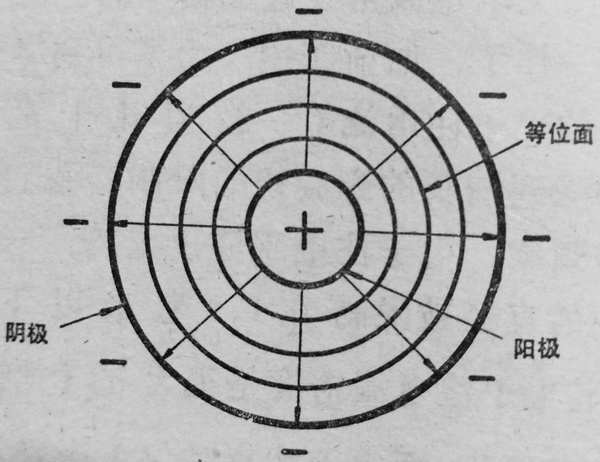
\includegraphics[width=0.42\linewidth]{figure/ch6-4}
	\caption{球形二极管电场分布示意图}
	\label{ch6-4}
\end{figure}

\begin{figure}[phtb]
	\centering
	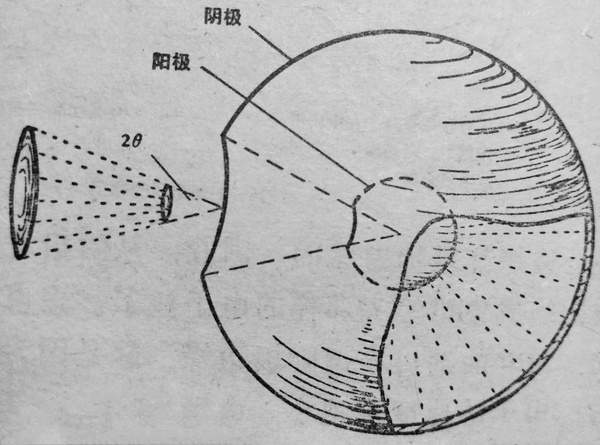
\includegraphics[width=0.5\linewidth]{figure/ch6-5}
	\caption{从球形二极管中取出一个圆锥形二极管}
	\label{ch6-5}
\end{figure}

球形二极管是一个假想的二极管,它的结构如图\ref{ch6-4}所示。它是由两个同心球面电极构成的,外边大球的内表面为阴极,其上涂有发射材料,里面的小球是阳极,如果在两个电极上加上直流电压,它们之间就会产生球对称的辐射状电场,如图所示。在这个辐射电场的作用下,外球面(阴极)发射的电子就将沿着电力线射向内球面(阳极),从而形成了球对称的、会聚状的电子注。我们可以进一步设想,如果能够从球面二极管中挖出来一部分,使得它的外形像一个圆锥那样,如图\ref{ch6-5}所示,那么,它的电子流形状就和铅笔尖的形状很相像了。此时,阴极和阳极将是两个同心球面的一部分。这就是我们为什么要把阴极做成凹球面状的原因。聚束极的作用是什么呢?可以想象,只靠凹球面状阴极我们所能得到的,并不是会聚状的电子流而是象图\ref{ch6-6}(a)所示的向外发散的电子注,这是由于空间电荷排斥力造成的。由于这种空间电荷排斥力的影响,电场将发生畸变,电力线要发生弯曲,这种现象在电极边缘尤为严重(如图\ref{ch6-6}(a)所示)。我们知道,电子是在电力线所表示的电场作用下运动的,如果电力线发生弯曲,那么,电子注的形状也就要发生畸变,因而不能满足我们的要求。为了改变电极边缘附近的电场,使它符合我们的要求,人们经过计算和模拟,设计出一种电极,即所谓聚束极,通常它是一个轴对称的电极,在它的上面加上一定的电压以后,聚束极将对电场进行修正,使得阴极和阳极之间的电场,不论中间还是边缘都是辐射状的。因此,从阴极发射出来的电子注就能被压缩成象铅笔尖那样的电子注了。聚束极常常被做成漏斗状的,漏斗的细口靠近阴极边缘,这是因为离阴极表面越近的地方,电子的速度就越小,电子的密度比较大,空间电荷的排斥力也比较大,电子注向外发散的趋势也强一些,因此,要求聚束极离阴极近些,以便对电子注施加较大的会聚力。理论计算得到,聚束极的漏斗斜面应当与电子注边缘成67.5$  {}^{\circ}$的夹角才能保证电子注有良好的会聚形状。为了使用和生产方便起见,聚束极的电位常常和阴极相同,但也有比阴极电压稍高或稍低的,这要由不同的设计要求来决定。

\begin{figure}[phtb]
	\centering
	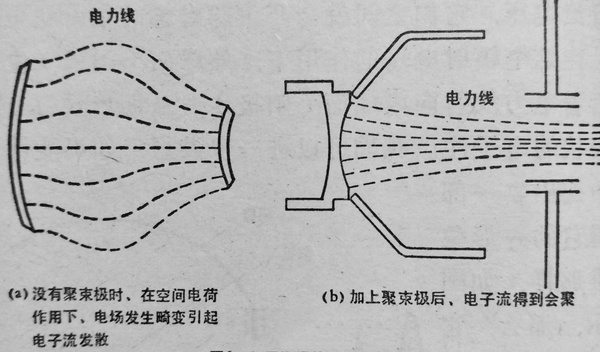
\includegraphics[width=0.75\linewidth]{figure/ch6-6}
	\caption{聚束极的作用}
	\label{ch6-6}
\end{figure}

对于阳极的形状,是这样考虑的:我们分析球面二极管并导出圆锥二极管并不是单纯为了设计一个圆锥二极管,而是要得到一束铅笔尖状的电子注。因此,阳极中心必须开孔,以便让电子注通过。阳极中心开孔对于电子枪区的电场略有影响(所谓阳极孔效应),但是通常不大。由于阳极对电子枪区电场的影响要比聚束极小得多,因此,为了加工方便起见,阳极不必做成球面状,常常做成一个中心开孔的圆片镶上一段小圆筒,如图中所示。或者干脆只做成一个中心开孔的圆片,中心孔附近略微有些斜面状就可以了。

这样由凹球面状的阴极、漏斗状的聚束极和中心开孔的圆片状阳极组成的电子枪就能够成功地得到铅笔尖状的会聚电子注,并达到高速细束的要求。

顺便提一点,细束电子枪的阴极面是一个不大的平面,聚束极是一个顶部中心开孔的中空圆筒,如图\ref{ch6-3}(b)所示。这是因为细束电子枪电子注电流很小的缘故。细束枪电子注内的空间电荷影响很小,通常可以忽略。

\section{怎样得到一把好的电子枪}

从前面的分析中我们知道,在行波管中,为了得到符合要求的强流电子注,常常采用轴对称收敛注电子枪,这种电子枪有下列优点:
\begin{enumerate}
	\item 收敛注电子枪能得到比阴极发射密度大得多的注电流密度,因此很容易满足行波管对电子注的要求。 
	\item 收敛注电子枪的阴极负荷较轻,因此,有利于延长阴极的寿命。
	\item 收敛注电子枪得到的电子注横向速度较小,因而使电子注聚束所需的磁场较小
\end{enumerate}

\subsection{对电子枪的基本要求}

对电子枪的基本要求归纳起来有下面几点:
\begin{enumerate}
	\item 电子注电流和电压(阳极电压)或导流系数应满足高频系统提出的要求。阳极上截获的电流越小越好。
	\item 电子注直径应满足高频系统提出的要求。因为高频系统决定后螺旋线的尺寸也就定了,因此电子注的直径便可决定。
	\item 电子注进入聚束磁场时应尽可能与轴线平行,电子注的层流特性要好。
	\item 工艺上容易实现,结构要牢靠。
\end{enumerate}

\subsection{电子枪的参量}

实际的电子枪是如何满足这些基本要求的呢?在回答这个问题之前,我们再来看一下在第\ref{ch4}章中提到的电子枪的导流系数$ P_\theta $。

我们知道,任何电子枪,如果画出它的伏安(阳极电压\textasciitilde 电子注电流)特性的话,都服从一条共同的规律:电流与电压的二分之三次方成正比。这个规律,我们称它为二分之三次定律,它的数学表达式是:
\begin{equation} \label{eq:ch6-1}
	I=P_\theta U^{3/2} \qquad\textrm{或}\; P_\theta = \frac{I}{U^{3/2}}
\end{equation}

式中:导流系数$ P_\theta $是一个常数,在电子枪的结构确定以后,导流系数也就定了。

导流系数有什么物理意义呢?

\begin{enumerate}
	\item 导流系数表征了电子枪在一定加速电压下给出电流的能力。$ P_\theta $越大,则在同样加速电压下,电子枪产生的电子注电流就越大;或者在同样电子注电流下,所需的加速电压就越低。$ P_\theta $对行波管许多重要指标,如增益、功率、效率等都有重大的影响,因此是电子枪最重要的参量。提高导流系数往往是改进行波管的一条重要途径
	\item 导流系数表征了电子枪中空间电荷作用的程度。$ P_\theta $越大,表示在同样电子注电压下电子注电流越大,也就意味着电子注中空间电荷密度$ \rho $越大,因此,形成锥形电子注所遇到的困难也越大。当$ P_\theta > 1$微朴后,空间电荷密度很大:各种矛盾将要激化,必须考虑更多的因素,对电极作各种修正。因此,高导流系数的电子枪的结构就比较复杂。我们常常把强流电子枪按$ P_\theta $的大小分成两大类:$ P_\theta =0.1\textasciitilde 1$微朴,称为低导枪。中、小功率行波管中多用这种枪,它的结构比较简单。$ P_\theta =1\textasciitilde 2$微朴或更大,称为高导枪。多用于大功率行波管或其它微波管中,结构比较复杂。
	\item 导流系数还表征了电子枪的结构情况与尺寸大小。$ P_\theta $大,阴极与阳极距离一定较近。$ P_\theta $大,电子注半锥角$ \theta $一定较大,即阴极直径较大。 
\end{enumerate}

对于本书重点介绍的行波管,其电子枪导流系数都很低因此可以采用结构比较简单的低导枪。典型的低导枪结构如图\ref{ch6-7}所示。它们的结构尺寸是怎样确定的呢?

\begin{figure}[phtb]
	\centering
	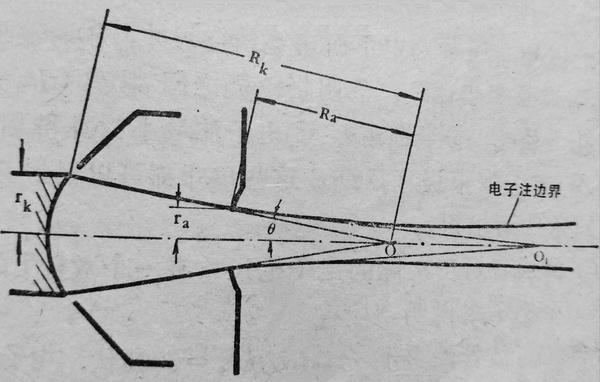
\includegraphics[width=0.65\linewidth]{figure/ch6-7}
	\caption{典型的低导枪结构示意图}
	\label{ch6-7}
\end{figure}


一个管子的高频系统设计完毕以后,电子注电压$ U_0 $、电子注电流$ I_0 $和电子注半径$ r_b $就知道了。于是我们可以算出它的导流系数$ P_\theta = \frac{I_0}{U^{3/2}} $

若阴极面半径为$ r_K $,那么阴极的支取电流密度就是$ J_K = \frac{I_K}{\pi r_K^2} $,式中阴极电流$ I_K$即电子注电流$ I_0 $(假定阳极电流等于零)。我们可以根据阴极的性能选择一个合适的$ J_K $值(例如200 mA/cm$ ^ 2$),于是由公式$ r_K = \sqrt{\frac{I_K}{\pi J_K}} $便可决定阴极面半径。

根据$ r_K $和$ r_b $我们可以求得电子枪的面压缩比$ M_{\textrm{面}} $,这是电子枪的另一个参量,它的定义是电子注电流密度与阴极电流密度之比,因此有:
\begin{equation} \label{eq:ch6-2}
	M_{\textrm{面}} = \frac{\left(\frac{I_K}{\pi r_b^2}\right)}{\left(\frac{I_K}{\pi r_K^2}\right)} = \frac{r_K^2}{r_b^2}
\end{equation}
面压缩比表征了电子注的收敛程度。我们还常用到线压缩比$ M_{\textrm{线}} $,$ M_{\textrm{线}} $定义为:
\begin{equation} \label{eq:ch6-3}
	 M_{\textrm{线}}  = \frac{r_K}{r_b}
\end{equation}

除此以外,还要确定下面这些结构尺寸:(1)阴极曲率半径$ R_K $,(2)阳极曲率半径$ R_a $,(3)阴极阳极之间距离($ R_K-R_a $)(4)阳极孔半径$ r_a $,(5)半锥角$ \theta $,(6)电子注最小截面和阳极之间的距离$ Z_{\textrm{min}} $,(7)聚束极直径$ D_g $。这些尺寸都可以根据$ P_\theta $、$ r_b $、$ r_K $等已知条件而求得。

为了使读者对于实际的电子枪尺寸有一个数量上的概念我们举一个例子来说明。

已知某行波管的电子注电压为$ U_0 = 3000 $\,V,电子注电流为$ I_0 = 25 $\,mA,电子注半径为$ r_b = 0.55 $\,mm。我们来计算其电子枪尺寸。

\begin{enumerate}
	\item 算出导流系数$ P_\theta $。
	\begin{equation*}
		P_\theta = \frac{I_0}{U_0^3/2} = 0.153\,\textrm{微朴}
	\end{equation*}
	可见,它的导流系数很低,是低导枪。
	\item 确定阴极半径$ r_K $。
	采用氧化物阴极,选取其支取电流密度为$ J_K = 150 $毫安/厘米$ ^2 $,则可算得:
	\begin{equation*}
		r_K = \sqrt{\frac{I_0}{\pi J_K}} = 0.23\,\text{cm} = 2.3\,\textrm{mm}
	\end{equation*}
	取$ r_K = 2.5 $毫米,即直径$ d_K = 5 $毫米。
	\item 求出压缩比。
	
	面压缩比$ M_{\textrm{面}} = \dfrac{r_K^2}{r_b^2} = \left(\dfrac{2.5}{0.55}\right)^2 = 4.55^2 = 20.7$
	
	
	线压缩比$ M_{\textrm{线}}  = \dfrac{r_K}{r_b} = 4.55 $
	
	一般认为,随着压缩比和导流系数的增加,阴极发射不均匀程度和电子注中非层流性将增加,电子注的形状尺寸对阴极表面发射情况的变化也越敏感,容易产生散焦(关于散焦,下章将讲到)。因此对于长寿命行波管,我们要求:面压缩比$ M_{\textrm{面}} < 25\textasciitilde 30$,导流系数$ P_\theta < 0.3 $微朴。
	\item 确定收敛半角$ \theta $(即半锥角)。
	
	选用氧化物阴极,取其工作温度$ T_K =\SI{750}{\degreeCelsius}= \SI{1023}{\kelvin} $,算出$ \sqrt{\frac{U_0}{T_K}} $。由$ \sqrt{\frac{U_0}{T_K}} $和$ M_{\textrm{线}}$查曲线得到$ \frac{R_K}{R_a }= 2.64$。由公式算得$ \theta =\SI{11}{\degree}\SI{6}{\arcminute}$。
	\item 确定阴极曲率半径$ R_K $。
		\[ R_K = \frac{r_K}{\sin \theta} = 13\,\textrm{mm} \]
	\item 求出阳极曲率半径$ R_a $和阳极孔半径$ r_a $。
	
	由$ \frac{R_K}{R_a} = 2.64$可求得$ R_a = \frac{R_K}{2.64} = 4.92$\,mm。
	
	$ r_a = R_a\cdot\sin\theta \approx1\,\textrm{mm} $,扩孔15\%,取$ r_a=1.15 $\,mm。
	\item 求出阴极与阳极之间的距离$ (R_K-R_a) $。
	
	$ R_K-R_a=13-4.92\approx 8.1 $\,mm。
	\item 求出电子注最小截面和阳极之间的距离$ Z_\textrm{min} $。
	
	查曲线后算得$ Z_\textrm{min}\approx 10 $\,mm。
	\item 聚束极直径$ D_g $取11.6毫米。
\end{enumerate}



这样,我们就把电子枪的尺寸大致确定下来了。应当指出,我们上面仅仅介绍了大致的计算步骤,计算是极粗略的在实际的电子枪设计计算中,往往要经过反复的理论计算和实验修正,才能得到一把理想的电子枪。

近年来,在电子枪的设计中已经广泛地采用了电子计算机,它可以给出精确的计算结果,并画出电子注的轨迹,从电子注轨迹中可以看出电子注层流特性是否良好。

求得了上述一系列尺寸以后,我们便可以根据这些尺寸做出电子枪来,并对它进行电参数测试,必要时还要反复修改电极尺寸和形状,最后才能得到一把符合我们要求的电子枪。


\section{两个问题}

我们在前面的叙述中曾经提到电子注的层流特性以及阳极孔效应等,它们是怎么一回事呢?

\subsection{电子的热初速}

使电子注发散的原因,除了空间电荷的排斥力外,还有电子的热初速,因此我们需要专门介绍一下。虽然空间电荷排斥力是发散的主要因素,但是当空间电荷所引起的发散力被克服以后,电子的热初速这个次要因素便突出出来了。它会影响计算的准确性,引起误差。特别是在阳极电压较低、电子注较细的情况下,这个次要因素的作用就更突出了。

所谓热初速,是指电子从热阴极发射出来时由于热运动而具有的初速度。我们知道热运动是杂乱的无规则的,因此,这些电子的运动方向(也就是速度方向)也是各不相同的。有沿轴方向的,也有沿电子注截面半径方向的(即所谓横向的热初速),后者将是引起电子注发散的一个因素。横向热初速的主要影响是:

\begin{enumerate}
	\item 横向热初速引起电子轨迹的偏离。电子的热初速都不算大,它相当于0.1伏的阳极电压所产生的速度。因此,如果是沿轴方向的,那么和一千伏以上的阳极电压比较起来是微不足道的,可以不予考虑。但是问题在于那些沿半径方向运动,或者说有径向速度分量的电子,它们的速度虽然不大,但是在飞离阴极后,由于横向速度的存在,它们就要偏离轴线向外运动,这就会影响电子注的会聚,起了附加的发散作用。在实际设计中就必须对这个由于电子横向热初速引起的轨迹偏离进行计算。
	\item 横向热初速造成电子注截面中电流密度分布的不均匀。从理想的电子枪中出来的电子注,其速度和密度都是均匀的。但是,由于电子横向热初速的存在,会使电子注的密度不均匀,同时还使原来很清晰的边界向外扩散,使边界变得模糊我们在设计电子枪时,考虑到这个因素的影响,应该把算得的电子注直径适当放大些。
\end{enumerate}

\subsection{层流特性}

我们观察小溪流水时可以发现有两种情况:一种是所谓层流”,在这种情况下,水流是很平稳的,好像分成若干层那样往前流动,它只有纵向流动而没有横向流动。另一种情况是“湍流”,此时,水流是起伏不平的,甚至有旋涡存在,这说明不仅有纵向流动而且有剧烈的横向流动。同样道理,我们希望电子枪产生的电子注也能够象层流的水流那样平稳地流动。这样,平行射入螺旋线中的电子注就能在纵向磁场的聚束下很好地与高频场交换能量。电子注层流特性好主要表现在电子没有横向运动,电子的轨迹没有交叉。如果层流特性不好电子存在着剧烈的横向运动,那么,电子就很容易打到阳极和螺旋线上去,因而和高频场相互作用的电子数就会减少。可见,改善电子注的层流特性是很重要的。

哪些因素会破坏电子注的层流特性呢?虽然电子横向热初速能够使层流特性变坏,但最主要的原因还是电子注的边缘电子经过阳极孔时所产生的影响。具体地说,离轴远的(电子注边缘的)电子受阳极孔的发散作用小,会聚角大,其轨迹如图\ref{ch6-8}(a)中的轨迹1;而离轴近的电子受阳极孔的发散作用大,会聚角小,其轨迹如图\ref{ch6-8}(a)中的轨迹2、3。从图\ref{ch6-8}(a)可以看到:由于阳极孔的影响,电子的轨迹发生了交叉,从而破坏了电子的层流性,在不同的电子注截面上,电流密度分布变得不均匀了。图\ref{ch6-8}(b)绘出了$ A $和$ B $两个截面上的电子的密度分布。在横截面$ A $处,电子注边缘是一个电流密度很大的圆环,而中心部分电流密度小。在横截面$ B $处,中心是一个电流密度很大的圆斑,其它地方电流密度都比较小。$ A $处和$ B $处的这两种情况,正如图中所示,是由于电子轨迹交叉引起的。实践证明,利用下面两种方法可以改善层流特性:

\begin{enumerate}
	\item 减小阴极曲率半径(即加大阴极半锥角$ \theta $)能改善电子注的层流特性。
	\item 采用阴极刮边的方法也可以改善电子注的层流特性。这是因为,电子轨迹的交叉主要是由于外层电子过于向内所造成的,所以我们很自然地会想到,把这些捣乱的外层电子去掉因此就采取了阴极刮边的办法,即将阴极边缘的发射物刮掉或者在阴极边缘嵌以无发射环。实践证明这个方法也是行之有效的。
\end{enumerate}


\begin{figure}[phtb]
	\centering
	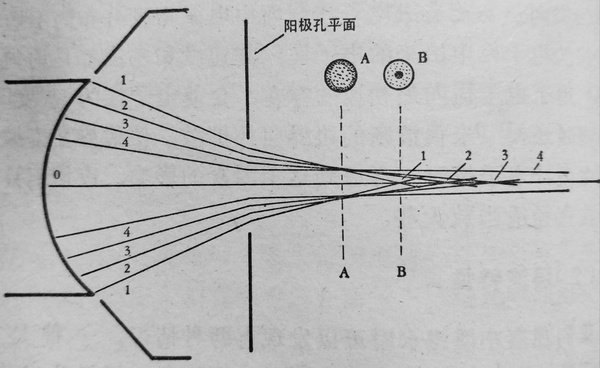
\includegraphics[width=0.85\linewidth]{figure/ch6-8}
	\caption{阳极孔对层流特性的影响}
	\label{ch6-8}
\end{figure}
\chapter{磁聚束系统} \label{ch7}

高速细电子注从电子枪中出来以后便进入互作用区(中间还有一个过渡区)并与螺旋线上传播的高频场发生持续的相互作用,最后在输出端得到放大的高频信号。为了使细电子注能够在细而长的螺旋线中有效地与高频场相互作用,我们必须设法不让电子打到螺旋线上去,使它能顺利地穿过螺旋线,这就是前面所说的如何“维持”电子注的问题。我们知道,螺旋线的长度一般要达到150\textasciitilde 200毫米以上,而直径只有1\textasciitilde 2毫米的细电子注内的电流密度又很大,其空间电荷排斥力也很大在空间电荷排斥力的作用下,细电子注将很快发散变粗,打到螺旋线上去,因而无法穿过细而长的螺旋线与高频场交换能量。另一方面,当我们在输入端送入高频信号时,高频场将沿螺旋线向前传播,并与细电子注相互作用,共同增长。在高频场的同步作用下,细电子注很快地群聚起来。随着群聚的不断增长,群聚电子注内的空间电荷密度也不断增大,其空间电荷排斥力不断增强,这样就在原来发散的基础上增加了一个新的发散力,由于这个发散力是加入高频信号以后才产生的,因此就把它叫做“动态散焦力”。可以看出,动态散焦力实质上也是空间电荷排斥力。

为了使细电子注的直径维持不变,以便有效地与高频场交换能量,我们必须设法在细电子注上面加上一个聚束力,来抵消前面所分析的两种空间电荷排斥力。这个聚束力通常是由外加轴向磁场来产生的,下面将要讲到,轴向磁场对于轴向运动的电子没有作用,但对于径向发散的电子却能够把它们拉回来。这种维持细电子注的方法就称为磁聚束方法,而产生轴向磁场的装置便叫做磁聚束系统。除了磁聚束以外,我们还可以用外加电场的方法来产生聚束力,称为电聚束。磁聚束和电聚束都有好几种方法,本章着重介绍中小功率行波管中最常用的周期永磁聚束法。

怎样才算是一个好的聚束系统呢?

\begin{enumerate}
	\item 聚束系统的好坏主要应当表现在电子注的流通率是不是高?电子注的流通率是指收集极电流$ I_c $占总的阴极电流$ I_K $的百分比。如果阳极电流等于零的话,阴极电流$ I_K $应等于收集极电流$ I_c $和螺旋线电流$ I_H $之和,因此,电子注流通率可以表示为$ \frac{I_c}{I_c + I_H} \times 100\%$,它的物理意义是进入螺旋线的电子注有百分之少能穿过整个螺旋线参予与高频场相互作用的过程。显然我们希望这个百分比越高越好,通常都在90\textasciitilde95\%以上。
	\item 细电子注在螺旋线中流动时应该有良好的稳定性,这样,行波管的工作才能稳定。
	\item 聚束系统的体积要小,重量要轻。这样有利于整个行波管的小型化。
	\item 聚束系统的磁性材料应尽可能做到性能好,来源多,价格便宜,制造工艺简单。
\end{enumerate}

\section{均匀磁场中的电子运动}


磁场对运动着的电子的作用力是克服电子束发散的关键力量。因此,弄清磁场(这里所说的磁场就是磁感应强度)、电子运动速度和磁场加给运动着的电子的作用力这三者之间的关系是很重要的。首先让我们从均匀磁场着手。

如果磁场中任何一点磁感应强度$ B $的大小和方向都完全相同,则该磁场称为均匀磁场。电子在均匀磁场中的运动可以分为三种情况。

第一种情况:带有电荷为$ -e $的电子在垂直于均匀磁场$ B $的平面中以速度$ v $运动。此时,磁场将对运动的电子产生一个作用力$ F $,它的大小等于$ evB $。$ F $的方向则是既和$ B $的方向垂直,又和$ v $的方向垂直,且应服从右手定则,如图\ref{ch7-1}所示。右手定则的意思是:任何电荷$ q $在磁场$ B $中以速度$ v $垂直于$ B $运动时,将受到磁场力$ F $的作用。如果四指从$ v $的方向向$ B $的方向转动,那么拇指的方向就是磁场作用力$ F $的方向。当$ q $是负电荷时$ F $的方向就与拇指的指向相反。由于电子电荷是$ -e $,因此,它受到的作用力$ F $的方向也应当与拇指的指向相反。

\begin{figure}[phtb]
	\centering
	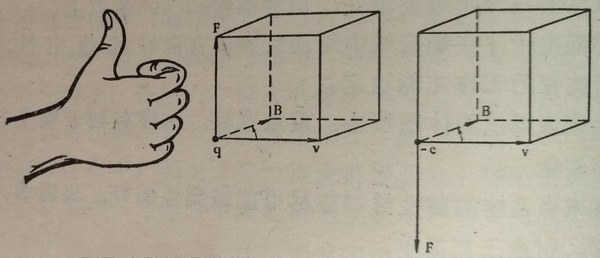
\includegraphics[width=0.8\linewidth]{figure/ch7-1}
	\caption{ 右手定则:四指从$ v $的方向向$ B $转动,拇指方向就是施加在正电荷$ q $上的磁场作用力$ F $的方向,如何电荷为负,$ F $的方向倒转}
	\label{ch7-1}
\end{figure}

在$ F $的作用下,真空中电子的运动将发生什么变化呢?由于$ F $的作用方向垂直于电子运动的方向,因此电子就将在垂直于磁场的平面中作圆周运动,这个情况就象一个人手中拿着条一端系有铁球的铁炼在空中划圈圈那样(图\ref{ch7-2})。人手通过铁练对铁球施一拉力$ F $,这个力就是铁球圆周运动的向心力,它垂直于铁球速度$ v $。同样,磁场力$ F $也是电子圆周运动的向心力,它只改变电子的运动方向而不改变电子运动速度的大小,因而不改变电子的动能。

\begin{figure}[phtb]
	\centering
	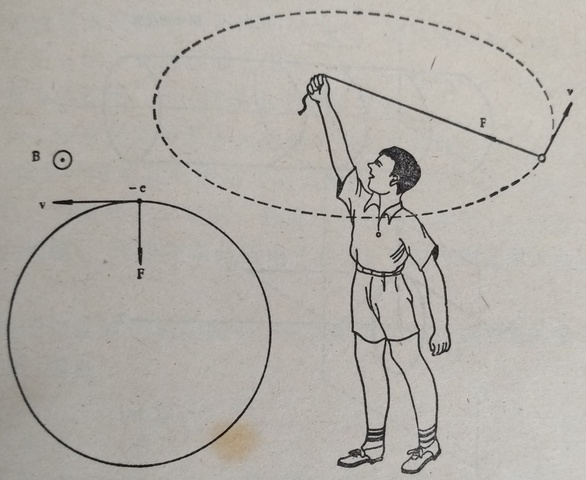
\includegraphics[width=0.75\linewidth]{figure/ch7-2}
	\caption{磁场作用力$ F $垂直于电子运动方向,使电子在垂直于磁场的平面中作圆周运动}
	\label{ch7-2}
\end{figure}

第二种情况是电子速度$ v $的方向与均匀磁场$ B $的方向平行,此时,磁场对电子没有作用。

第三种情况是最一般的情况:电子的运动方向既不和均匀磁场平行又不和均匀磁场垂直(图\ref{ch7-3})。设均匀磁场$ B $的方向是正$ Z $方向,此时我们可以把电子速度$ v $分解成与磁场方向(即$ Z $轴方向)平行的分量$ v_z $以及与磁场方向垂直的分量$ v_{xy} $(即在$ xy $平面内的分量)。磁场对$ v_Z $无作用(因此电子的$ Z $向速度$ v_z $保持不变),但是对$ v_{xy} $将产生作用力$ F_{xy} = e\cdot v_{xy}\cdot B $在$ F_x $的作用下,电子在$ xy $平面内作圆周运动,因此电子的运动就是它在$ Z $轴方向的直线运动和$ xy $平面内的圆周运动的合成,这个合成运动的轨迹是一根螺旋状的曲线,电子好像在一个假想的圆柱面上一边旋转一边沿$ Z $轴向前运动。由此可见,如果有一个本来要离开$ Z $轴向外飞出去的电子,那么,在轴向磁场的作用下,它的运动就将变为沿$ Z $轴作螺旋运动了。这就是说,轴向磁场已经把电子的运动约束在一个圆柱面范围内了。

\begin{figure}[phtb]
	\centering
	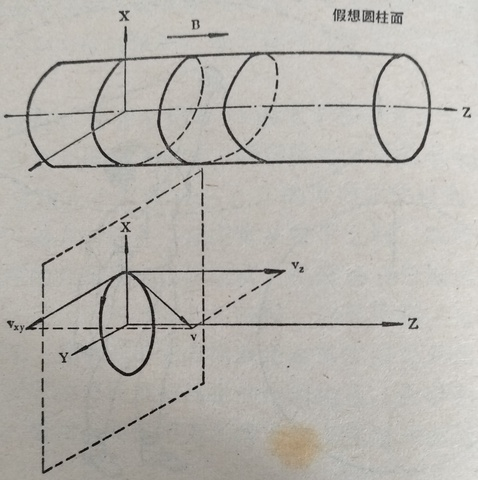
\includegraphics[width=0.6\linewidth]{figure/ch7-3}
	\caption{电子在均匀轴向磁场中作螺旋运动}
	\label{ch7-3}
\end{figure}

把上面的分析用到实际的电子注中去,就能发现磁场对电子注的聚束作用。

我们知道,电子注内的电子受到较强的空间电荷排斥力的作用向外发散,这就说明电子得到了横向速度。如何对付这些发散的电子呢?我们把前面对第三种情况的分析应用于这些发散电子,可见,只要在电子注运动空间加上一个轴向磁场$ B $,就可以使这些发散电子不再向外飞去,而是被约束在假想的圆柱面上沿$ Z $轴作螺旋运动(图\ref{ch7-3})。因此,轴向磁场就起到了聚束的作用,$ F_{XY} $就是电子的聚束力。

为了知道究竞需要多大的轴向磁场才能有效地对电子注聚束,就要弄清楚轴向磁场与电子螺旋运动的关系,例如,电子每打一圈需要多少时间?螺旋运动的半径有多大?等等。为了简化问题,我们先来分析电子在$ xy $平面内作圆周运动的情况。

电子作圆周运动的向心力就是轴向磁场对运动着的电子的作用力,因此,
\begin{equation} \label{eq:ch7-1}
	\frac{mv_{xy}^2}{r} = ev_{xy}B
\end{equation}
式中:$ m $是电子质量,$ r $是圆周运动的半径。由上式可得:
\begin{equation} \label{eq:ch7-2}
	r = \frac{mv_{xy}}{eB}
\end{equation}

圆周运动的周期(即电子飞行一圈所需的时间)为:

\begin{equation} \label{eq:ch7-3}
	T = \frac{2\pi m}{eB}
\end{equation}

这些关系式能不能用到电子的螺旋运动中去呢?我们知道,电子的螺旋运动是轴向(即纵向)直线运动和横向圆周运动的合成。因此,电子的轴向位移将由$ v_z $决定,而横向位移则由$ v_{xy} $和$ B $来决定,也就是说电子的螺旋半径应当等于圆周半径$ r $,螺旋运动的周期应当等于圆周运动的周期$ T $,螺旋运动的螺距$ L $应当等于周期$ T $和轴向速度$ v $的乘积(螺距等于经过一个螺旋周期后电子的轴向位移)。它们的数学表达式分别为:
\begin{equation} \label{eq:ch7-4}
	\begin{aligned}
	r &= \frac{mv_{xy}}{eB}\\
	T &= \frac{2\pi m}{eB}\\
	L &= v_zT = v_z\frac{2\pi m}{eB}
	\end{aligned}
\end{equation}

这是三个基本的关系式,从这三个关系式中我们可以得出几点结论:

\begin{enumerate}
	\item 电子螺旋运动的半径和它的横向速度$ v_{xy} $成正比,和磁感应强度$ B $成反比。因此在一定的磁场下,电子的横向速度越大(发散越严重),螺旋运动的半径就越大。另一方面,磁场越强,电子的螺旋运动半径就越小,也就是旋转的圈圈越由此可见,为了有效地约束发散电子,就应当增强磁场。
	\item 电子的螺旋运动周期仅仅和磁场大小有关,而和电子的速度无关。 \label{item:ch7-1}
	\item 电子螺旋运动的螺距仅仅和磁场大小、电子的轴向速度有关,而和电子的横向速度无关。\label{item:ch7-2}
\end{enumerate}



\begin{figure}[phtb]
	\centering
	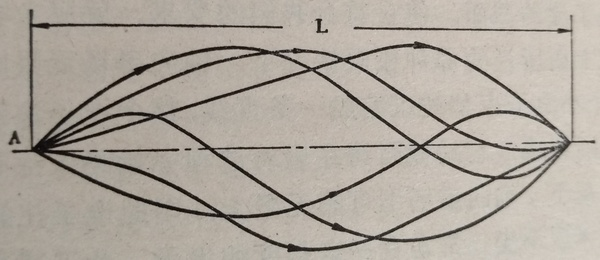
\includegraphics[width=0.6\linewidth]{figure/ch7-4}
	\caption{电子在均匀磁场中会聚示意图}
	\label{ch7-4}
\end{figure}

把上面\ref{item:ch7-1}、\ref{item:ch7-2}两个结论用到实际的电子注中去是很有趣的。我们假定在某一个瞬间有许许多多电子以各不相同的横向速度同时从$ A $点出发向前飞去,它们将在同一个轴向磁场的作用之下,沿$ Z $轴方向作各自的螺旋运动,由于它们的横向速度各不相同,因而螺旋的半径也各不相同。但是它们的螺旋运动周期却是相等的,这就是说它们将同时旋转完一圈,同时开始转第二个圈,同时转完第二圈,这样依次下去。更加有趣的是,由于电子注中的电子都是在同一个加速电压下得到加速的。因此它们的$ Z $向速度$ v $可以认为是相等的,由\ref{eq:ch7-4}式可知,它的螺距$ L $也应该相等。因此,从$ A $点同时出发的许多电子,经过一个周期以后,将同时到达某一点$ A' $,$ A $点和$ A' $点之间的距离等于螺距$ L $,如图\ref{ch7-4}所示。图\ref{ch7-4}再次体现了轴向磁场对发散电子的聚束作用。图中从$ A $点出发的许许多多电子构成了一个很小的电子束,电子束的外径是由横向速度最大的那些电子决定的。因此为了减小电子束的外径就希望增大磁场,使得横向速度最大的那些电子的运动半径在强磁场作用下变得很小,那么横向速度较小的那些电子的运动半径就更小了。图\ref{ch7-5}表示了小电子束截面大小和轴向磁场的关系,在极限情况下,$ B \to \infty $,小电子束被压缩成一条直线。

\begin{figure}[phtb]
	\centering
	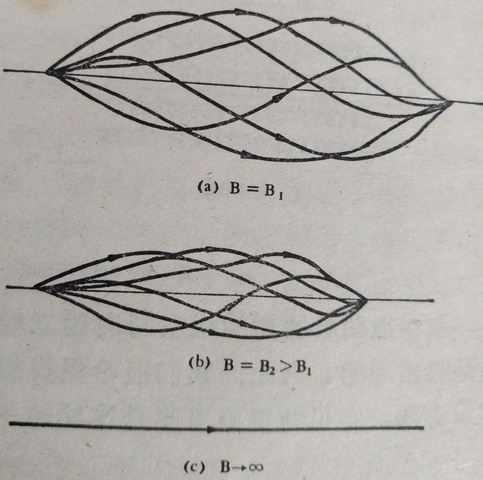
\includegraphics[width=0.55\linewidth]{figure/ch7-5}
	\caption{小电子束截面的直径随轴向磁感应强度的增大而减小}
	\label{ch7-5}
\end{figure}

\begin{figure}[phtb]
	\centering
	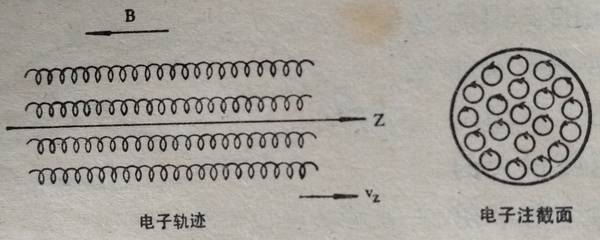
\includegraphics[width=0.65\linewidth]{figure/ch7-6}
	\caption{暴力聚束中的电子轨迹}
	\label{ch7-6}
\end{figure}

实际的电子注截面中存在着许许多多个“$ A $点”,因此,整个电子注可以看成是由许许多多小电子束所组成的。为了减小整个电子注的截面,使它符合我们的要求,就应当增大轴向磁场。在上面所说的那种极限情况下,轴向磁场无限增大,此时,每一个小电子束都被压缩成一条直线,整个电子注就将由无数条直线所组成,它的截面将在运动过程中始终保持不变。但在实际情况下,轴向磁场不可能无限大,因此电子注的截面将不能始终保持不变,常常有一定程度的发散,为了减小这种发散,就必须尽量增大轴向磁场。因此,所需要的磁感应强度是很大的。这种聚束方法叫做暴力聚束或磁限制流聚束。在暴力聚束的电子注中,电子运动的特点是沿着各自的磁力线作螺旋运动即打小圈圈,如图\ref{ch7-6}所示。暴力聚束的最大缺点是所需的磁场要很强,高达几千高斯。

要在细而长的螺旋线空间内建立起高达几千高斯的聚束磁场是很困难的。因此,我们很希望找到一种聚束磁场比较低的聚束方法。布里渊流聚束便是这样的一种聚束方法。

\section{布里渊流聚束}

\subsection{什么叫布里渊流聚束}

我们知道,电子注从电子枪出来尚未射入螺旋线时,由于电子枪内静电场产生的会聚力和电子注内空间电荷发射力相平衡,电子注中的电子便只有轴向速度,没有径向速度。但是电子注射入螺旋线后静电场会聚力便没有了,而空间电荷发射力却依然存在,因此电子注就要发散,它的主要表现是电子注的径向扩张。在发散力作用下,电子有了径向速度。如果我们采用暴力聚束,那么强大的轴向磁场便立刻把电子的径向运动局限在很小的空间内,变成沿磁力线的很小的螺旋运动,在整个电子注中,无数个电子便将围绕着无数根磁力线打着小圈圈前进。

从\ref{eq:ch7-2}式可知,为了使电子打小圈圈前进必须用很强的磁场,这就是暴力聚束需要强磁场的原因。因此我们想,要是能够用打大圈圈的办法来约束电子使它不发散,那么所需的磁场不是可以小得多吗?不过,如果象暴力聚束中那样,电子还是各自绕着各自的磁力线打圈圈,那么圈圈打大了只会使整个截面增大,起不到聚束的作用。我们知道,行波管中的电子注是轴对称电子注,因此,如果能够让所有的电子都绕着共同的轴(即电子注的轴)打圈圈,不也能把它们约束在电子注所占据的范围内吗(图\ref{ch7-7})?而这时由于圈圈要比暴力聚束大得多,因此所需的轴向磁场就可以比暴力聚束时小得多,这的确是一个很好的想法。但是怎样使所有电子都围绕着对称轴打圈圈呢?我们采用了径向磁场的办法。这就是在电子注进入螺旋线时在螺旋线前面利用极靴来得到一个轴对称的径向磁场$ B_r $,极靴是用高导磁率的纯铁制成的,磁力线能够高度的集中到它里面去。由于它的存在,就使轴向磁场的磁力线发生急剧的弯曲,从而产生了轴对称的径向磁场。如图\ref{ch7-8}所示。

\begin{figure}[phtb]
	\centering
	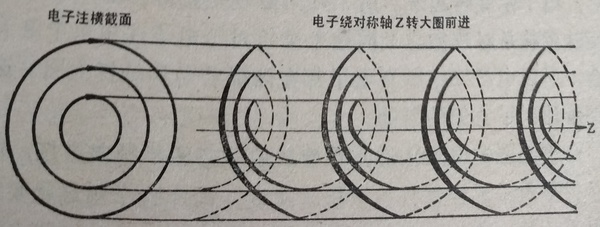
\includegraphics[width=0.85\linewidth]{figure/ch7-7}
	\caption{使电子绕对称轴转大圈以便减小所需要的轴向磁感应强度}
	\label{ch7-7}
\end{figure}

\begin{figure}[phtb]
	\centering
	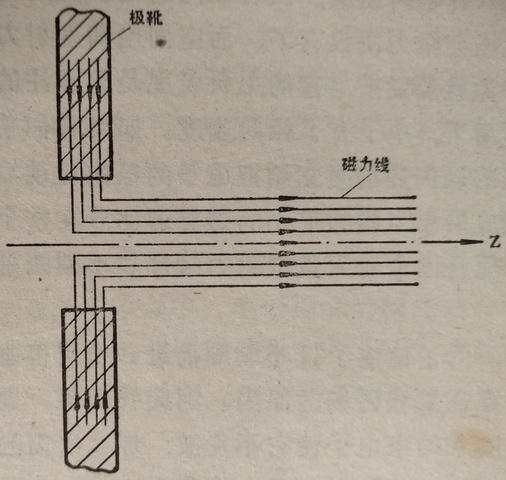
\includegraphics[width=0.65\linewidth]{figure/ch7-8}
	\caption{极靴使磁力线弯曲产生径向磁场}
	\label{ch7-8}
\end{figure}

现在我们来分析一下平行电子注进入图\ref{ch7-8}所示的聚束磁场时的情况。平行电子注首先碰到的是轴对称的径向磁场$ B_r $,在$ B_r $的作用下,根据右手定则,电子受到了切向力$ F_\theta $,因而产生了切向速度$ v_\theta $(我们又称它为旋转速度),有了旋转速度以后,电子便旋转起来。由于径向磁场是轴对称的,因此电子的旋转轴就是对称轴。上面这个分析对于电子注中每个电子都适合,所以电子注中所有电子都在围绕着对称轴打大圈。这样就初步达到了我们的目的。

打着圈圈的电子注进入螺旋线后就碰到了轴向磁场,由于此时每个电子已经都具备了旋转速度。因此这个磁场就要对每个电子作用,产生一个指向对称轴的聚束力,这就是说,电子注进入螺旋线以后,虽然失去了电子枪内的静电场会聚力,但是却由于旋转速度而得了轴向磁场的聚束力,这就给发散力和聚束力的平衡提供了可能。

我们来看看电子注内电子的受力情况。在这种情况下任何一个电子都要受到三种力:(1)空间电荷排斥力$ F_{\textrm{空}} $。半径$ r $处电子所受的空间电荷力$ F_{\textrm{空}} = \frac{eI}{2\pi \varepsilon_0 r \sqrt{2\eta U_0}}$。(2)电子绕对称轴旋转所产生的离心力$ F_{\textrm{离}} $,$ F_{\textrm{离}} = m \cdot \frac{v_\theta^2}{r}$。(3)轴向磁场产生的径向聚束力$ F_{\textrm{聚}} $,$ F_{\textrm{聚}} = ev_\theta B$。这三种力都是径向力。要使电子注的直径保持不变,电子注内各个电子所受到的各种径向力必须平衡,这样才能使电子注维持一定直径。我们考虑电子注边缘其半径为$ r_b $电子的受力情况,为了达到径向力平衡,下列等式必须成立:$ F_{\textrm{聚}}= F_{\textrm{空}} + F_{\textrm{离}}$,即:
$ ev_\theta B \lvert_{r = r_b} = \frac{m v_\theta ^2}{r}\lvert_{r = r_b} + \frac{eI_0}{2\pi\varepsilon_0 r \sqrt{2\eta U_0}} $,经过一些计算,最后可得到:
\begin{equation}   \label{eq:ch7-5}
	B_b = \frac{8.33\times 10^2}{r_b}\cdot \frac{I_0^{1/2}}{U_0^{1/2}}
\end{equation}
式中:$ r_b $:电子注半径,单位为厘米。$ I_0 $:电子注电流,单位为安培。$ U_0 $:电子注电压,单位为伏特。

可见,在这种情况下,为了得到无脉动的电子注,只需要$ B_b $这样大的磁场就行了。后面我们将讲到,聚束磁场太大了反而会引起电子注的脉动。这种聚束方法称之为布里渊流聚束,实现布里渊聚束所需要的磁场值便叫做布里渊磁场值$ B_b $。一般情况下,$ B_b $都在1000高斯以下,因此,比暴力聚束所需磁场要小得多。这一点也可以用“电子打大圈所需磁场要比打小圈时小”来解释。

在实际情况下,由于热初速和阳极孔效应,有一部分电子在进入螺旋线时具有横向速度,不能满足平行入射的要求,因此为了克服这些电子造成的发散,实际所需的磁场值常常为$(1.5\textasciitilde2) B_b $。

\subsection{电子注的脉动}

在实际的聚束系统中,电子注的脉动是难以完全避免的产生脉动的原因主要有:(1)聚束磁场不合适。(2)电子枪和聚束系统对中不良使电子注不能平行入射。(3)聚束磁场的不均匀性。(4)电子注电流本身的起伏。要使这些原因产生的脉动完全消除是极困难的,因此我们所做到的平衡只能是相对的平衡,而不平衡则是绝对的。

下面我们来分析一下单纯因为聚束磁场不合适而引起的电子注脉动。

我们关心的是电子注的直径变化,因此只要观察最外层电子的运动就行了。假定最外层电子以半径$ r_0 $平行入射(图\ref{ch7-9}),由于聚束磁场过强($ B>B_b $),磁聚束力$ F_{\textrm{聚}} $过大,因此使电子产生了向轴的径向速度$ v_r $和径向加速度$ a_r $,电子被拉向轴线,电子注截面就收细了。但是随着电子注截面的收缩,空间电荷的排斥力就要增大,同时$ F_\textrm{聚} $也要随着电子注截面的收细而减小,即聚束力要减小。因而就有可能使$ F_{\textrm{聚}} $和$ F_{\textrm{空}} $、$ F_{\textrm{离}} $达到新的平衡。

\begin{figure}[phtb]
	\centering
	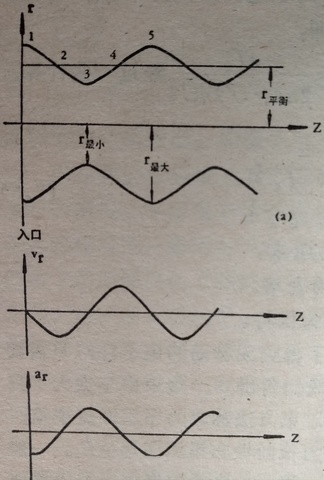
\includegraphics[width=0.45\linewidth]{figure/ch7-9}
	\caption{(a)电子注脉动示意图 (b) $ v_r $和$ a_r $沿$ Z $轴变化情况}
	\label{ch7-9}
\end{figure}


在脉动不大的情况下,最外层电子被拉到平衡半径(图\ref{ch7-9}中“2”点)时,$ F_{\textrm{聚}}$和$ F_{\textrm{空}} $、$ F_{\textrm{离}} $达到新的平衡,因此电子的径向加速度$ a_r=0 $,但此时它的径向速度$ v_r $却达到最大,所以由于惯性,电子还要往里跑,即电子注截面还要继续收缩。在继续收缩的过程中出现了新的不平衡,随着截面的收缩空间电荷发散力进一步增大,而磁场的聚束力却在减小,因此发散力要大于聚束力,出现了把电子往外拉的力,因而产生了离轴向外的径向加速度$ a_r $,电子向轴的径向速度$ v_r $就要减小。到达“3”点时电子的径向速度等于0,但$ F_{\textrm{空}} $达到最大,$ F_{\textrm{聚}} $达到最小,因而电子离轴向外的径向加速度达到最大,电子便要改变运动方向,离开轴线向外扩散。当电子到达“4”点时$ F_{\textrm{聚}} $与$ F_{\textrm{空}} $、$ F_{\textrm{离}} $再次达到平衡,径向加速度$ a_r $等于零,但径向速度$ v_r $达到最大,在惯性作用下电子继续向外运动,此时$ F_{\textrm{聚}} $和$ F_{\textrm{空}} $、$ F_{\textrm{离}} $又开始不平衡,$ F_{\textrm{聚}} $占优势。因而在电子的运动过程中将受到指向轴的径向加速度,电子离轴的径向速度$ v_r $逐渐减小到达“5”点时$ v_r=0 $,$ a_r $最大,电子在$ F_{\textrm{聚}} $的作用下将向内运动。此后的过程又和“1”到“5”点一样,如此反复循环下去。因此,电子注在向前运动的过程中,一会儿收缩一会儿发散,呈现出周期性的脉动。与此同时,电子注还要绕对称轴打圈圈,图\ref{ch7-10}形象地画出了电子注的脉动。

我们常常用脉动的振幅和脉动波长来描述脉动的大小。脉动的振幅是指最外层电子脉动的大小,在小脉动情况下,脉动是围绕着平衡半径进行的,平衡半径就是脉动的平均半径,这时脉动振幅为$ \frac{r_{\textrm{最大}} - r_{\textrm{最小}}}{2} $。脉动波长则是脉动一次前进的距离,如图\ref{ch7-9}中所示。脉动波长与磁场大小成反比,与电子注的加速电压的平方根成正比。

\begin{figure}[phtb]
	\centering
	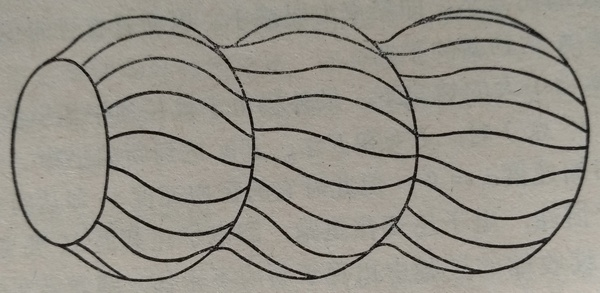
\includegraphics[width=0.5\linewidth]{figure/ch7-10}
	\caption{电子脉动形状示意图}
	\label{ch7-10}
\end{figure}
\section{周期永磁聚束}

布里渊流聚束解决了聚束磁场太大这个问题。接下来就是怎样产生所需要的布里渊磁场了。最初,人们是采用漆包线绕成的多层螺线管线包来产生轴对称磁场的,因而叫做线包聚束(见图\ref{ch7-11})。当线包导线内通以电流时,线包空间内就会产生轴对称磁场,把行波管插到线包的中心,磁场就能对电子注进行聚束。为了得到布里渊流,在电子进入螺旋线的入口处可加一极靴,从而方便地得到轴对称的径向磁场。但是,线包聚束有着很大的缺点:体积大、笨重、效率低。例如,个三厘米波段的小功率行波管,如果用多层线包来产生磁场,那么,线包的重量将达到30公斤,它所消耗的功率将达到400瓦,而行波管本身的重量不过几百克,所消耗的功率不过几瓦或几十瓦。同时,线包的外径也要比行波管大5—10倍。因此,现在已很少采用线包聚束,但这种聚束方法也有一个优点,即它所产生的磁场比较均匀,因此,电子注脉动小,噪声也小。
\begin{figure}[phtb]
	\centering
	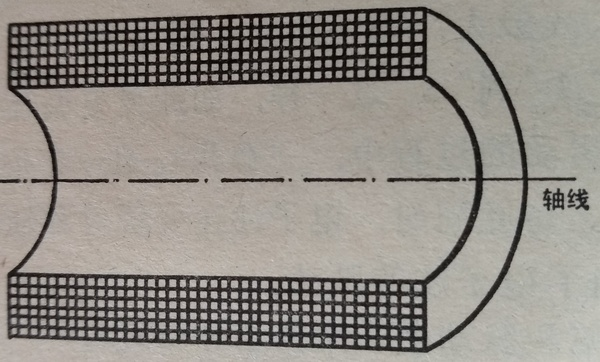
\includegraphics[width=0.47\linewidth]{figure/ch7-11}
	\caption{多层螺旋管线包绕组示意图}
	\label{ch7-11}
\end{figure}

能不能用永久磁铁来产生行波管所需要的轴对称磁场呢?人们曾经尝试过用圆环形永久磁铁(图\ref{ch7-12})来产生轴对称磁场。在磁环厚度不大的情况下,它所产生的轴向磁场沿轴线的分布可以做到比较均匀由于行波管电子注很长,因此也要求圆磁环的轴向长度很长,但是我们发现,随着圆磁环长径比(即磁环的轴向长度与直径之比)的增大,它所产生的磁场的轴向分布将越来越不均匀,这对电子注的聚束带来很大的不利。图\ref{ch7-13}表示了三种长径比情况下磁场的轴向分布。从曲线中可以看出长径比越大,中间跌落得越厉害,磁场越不均匀。
\begin{figure}[phtb]
	\centering
	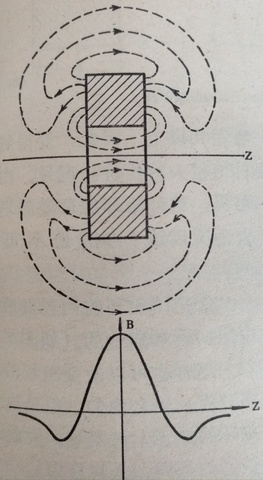
\includegraphics[width=0.35\linewidth]{figure/ch7-12}
	\caption{用环形磁铁产生轴对称轴向磁场}
	\label{ch7-12}
\end{figure}

\begin{figure}[phtb]
	\centering
	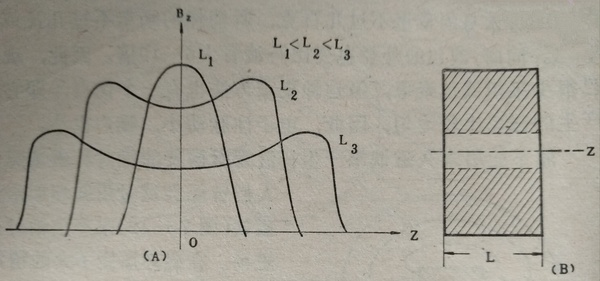
\includegraphics[width=0.65\linewidth]{figure/ch7-13}
	\caption{不同厚度磁环的轴向磁场分布}
	\label{ch7-13}
\end{figure}



为了使磁场的轴向分布尽量均匀,可以有两个办法:

\begin{enumerate}
	\item 增大圆磁环外径。但是这将大大增大磁环的体积和重量,例如,为了使磁场的均匀部分增长一倍,磁环的外径也需要增大一倍,而其体积和重量就将增加到八倍,也就是说,磁环的体积和重量将按长度的三次方成比例地增加。我们知道,行波管轴向长度很长,长径比一般在40以上,因此,要得到如此长的轴向分布均匀的磁场需要付出很大的代价。况且,由图可见,这种磁环的杂散磁场很大,所以这个办法是不可取的。
	\item 把圆磁环的内径做成自中间向两端渐变的(如图\ref{ch7-14})。这样也可以改变磁场的轴向分布,使之均匀。但是这种磁环的加工十分困难,因此这种方法也不可取。我们在实际中采用的是周期永磁聚束。
	\end{enumerate}
\begin{figure}[phtb]
	\centering
	\includegraphics[width=0.4\linewidth]{figure/ch7-14}
	\caption{用磨磁环方法实现均匀轴向磁场}
	\label{ch7-14}
\end{figure}
\subsection{什么叫周期磁场}

我们知道,长径比越大的磁环,其中间跌落也越大。这是什么原因呢?让我们先来做个实验:我们采用多个短磁环重的办法来得到不同长径比的长磁环,并分别画出它们中心磁场的轴向分布,如图\ref{ch7-15}所示。由此可见,单个磁环的磁场轴向分布是脉冲状的,中间有一个主峰,两旁则有两个对称的反峰(为什么产生反峰,见图\ref{ch7-17}。靠外层的磁力线沿$ Z $轴上的方向与磁环中心的磁力线方向相反)。如果我们把两个磁环重迭起来,异极性相对,那么,它们立刻会吸在一起,其合成磁场就应该是两个单磁环磁场之和。因此,合成磁场的轴向分布曲线就可以用两个单磁环的磁场分布曲线达加起来得到。实践证明,这样得到的分布曲线是和实际测得的分布曲线相符合的。可见,磁场中间跌落的原因就在于邻近磁环反峰的抵消作用。同理,我们可以画出由3个、4个以至$ n $个短磁环重选起来构成长磁环的中心磁场分布曲线,并且可以看出:磁环的长径比越大,那么磁场的中心跌落也越严重,举个例子来说,当长径比等于4时磁场就将跌落到原来的60\%。
\begin{figure}[phtb]
	\centering
	\includegraphics[width=0.65\linewidth]{figure/ch7-15}
	\caption{用短磁环重叠成不同长径比的长磁环}
	\label{ch7-15}
\end{figure}

于是人们就想,如果两个磁环,同极性相对地排列在一起,那么第2块磁环的反峰磁场就不但不会抵消第1块磁环的主峰磁场,而且可以加强第一块磁环的主峰磁场了(见图\ref{ch7-16})。但是要使两块磁环同极性面密合重达在一起是不可能的(斥力太大),只能使两块磁环间有一定的间距,而且这个间距不能太小,否则两个磁环的磁力线要“顶牛”,斥力太大,磁环就容易跑掉。可是间距如果太大,反峰加强主峰的优点就不能得到,磁场分布会更不均匀。怎样使两个磁环距离很近而又稳定地靠在一起呢?人们想了一个很巧妙的办法:在两块磁环中间夹一块纯铁制成的圆形铁片,叫做极靴,它的尺寸和磁环差不多。由于纯铁的导磁率很高,因此,极靴两边磁环产生的磁力线就不会“顶牛”,而且可以很容易地从共用的极靴当中穿过并进入磁环的内部空间,如图\ref{ch7-17}所示,这样,两块磁环就通过极靴紧密地排列在一起了。由于极靴的存在,磁环之间的间距就可以做到很小,例如在1毫米以下。这样就解决了两个磁环之间近距离地稳定地靠在一起的问题。那么极靴会不会使中心磁场减小呢?我们先来看一下单个磁环的情况,实验证明如果在单个磁环两端加上极靴,那么它们的中心磁场不但不会减小而且将得到提高,例如某单个磁环的中心主峰磁场为690高斯,两端加上极靴后就增加到800高斯,即增加了16\%。中心磁场增加的原因可以解释为加了极靴后磁力线向环内集中的结果。现在来看看多个磁环同极性相邻(中间加极靴)地排列在一起的情况,由于相邻磁环反峰和主峰的迭加,中心磁场便得到了加强,但相邻磁环产生的中心磁场是反向的,其轴向磁场$ B_z $的分布如图\ref{ch7-18}所示,可见这是一个周期性的分布,形状接近于正弦曲线,因此被称为周期磁场。周期磁场的峰值要比单个磁环时大很多,例如上例所举的磁环,单环两端加极靴后中心峰值磁场可增加16\%达到800高斯,组成周期磁场后峰值进一步增加到1000高斯,即又增加了25\%,这是很可喜的。在周期场中,为了增加磁场的轴向长度只需要适当增加周期数就可以了,增加的那部分磁场并不会影响原来磁场的轴向分布,整个磁场仍是周期性的。因此,我们不必担心会出现中间跌落的现象,当然也无需用增大磁环直径的办法来改进中间跌落了。相反的,由于磁力线向环内集中(即将无用的环外磁力线集中到环内变为有用),中心磁场反而加强了。而环外的磁力线则很少(相邻磁环产生的环外磁力线相互抵消及磁力线向环内集中两个原因导致),因此周期磁场的漏磁很小,这是它的一个优点。周期磁场的最大优点则是体积小、重量轻。例如,为了使磁场的轴向长度增加到原来长度的$ N $倍,对周期场来说,只要把周期数增加到原来的$ N $倍就可以了,因此其体积和重量都只增加到原来的$ N $倍。但是对均匀场来说,不但磁环的轴向长度要增加,而且磁环的直径也要增加到原来的$ N $倍,因此其重量和体积就要增加到原来的$ N^3 $倍。可见,周期磁场的重量和体积都要比均匀场小$ N^2 $倍,不过实际上一般不到$ N^2 $倍,约为$ N\textasciitilde N^2 $倍。举个例子,某行波管如用均匀场聚束,聚束系统重量需20公斤,但用周期场聚束,聚束系统只需0.5公斤。
\begin{figure}[phtb]
	\centering
	\includegraphics[width=0.37\linewidth]{figure/ch7-16}
	\caption{两块磁环同极性相对地排列在一起,则它们的反峰磁场相互加强相邻磁环的主峰磁场}
	\label{ch7-16}
\end{figure}

\begin{figure}[phtb]
	\centering
	\includegraphics[width=0.65\linewidth]{figure/ch7-17}
	\caption{加极靴后磁力线集中情况}
	\label{ch7-17}
\end{figure}

\begin{figure}[phtb]
	\centering
	\includegraphics[width=0.5\linewidth]{figure/ch7-18}
	\caption{周期磁场}
	\label{ch7-18}
\end{figure}

\subsection{电子在周期磁场中的运动}


周期磁场特别适宜于产生长径比较大的聚束磁场。为了弄清这种正弦形的周期磁场是怎样对电子注聚束的。下面就让我们分析一下电子注是如何在周期磁场中运动的。


可以分成三区来讨论:(1)会聚区


设电子注以某一半径$ r_{\textrm{最大}} $平行入射到周期磁场中(图\ref{ch7-19}),在磁场入口处轴对称径向磁场的作用下(为了实现布里渊流聚束,在入口处都设置了轴对称的径向磁场),电子得到了较大的旋转速度$ v_\theta $开始绕轴旋转。如果$ r_{\textrm{最大}} $是我们所允许的最大注半径,那么就必须把周期场的峰值轴向磁场放在1-1面处,此时,$ B_z $产生的聚束力$ F_{\textrm{聚}} $就达到最大,同时还应当使$ B_z $足够大,以保证$ F_{\textrm{聚}} >  F_{\textrm{空}} +  F_{\textrm{离}}  $,其中$ F_{\textrm{空}} $是电子注中的空间电荷排斥力,$ F_{\textrm{离}} $是电子绕轴旋转所产生的离心力。


因此,1-1面处作用在电子上的合力就是指向轴的聚束力,且为最大,电子得到了一个径向加速度$ a_r $,并产生了径向速度$ v_r $,因而电子注开始收细。


过了1-1面以后出现了反向的径向磁场($ B_r $变号),电子的$ v_\theta $就要减小,同时$ B_z $也渐渐减小,而随着电子注的收细$ F_{\textrm{空}} $将增大,当电子到达2-2面时将达到$ F_{\textrm{聚}} =  F_{\textrm{空}} +  F_{\textrm{离}}  $(此时电子注的半径等于平衡半径$ r_{\textrm{平衡}} $),因此,电子的径向加速度等于零。
\begin{figure}[phtb]
	\centering
	\includegraphics[width=0.37\linewidth]{figure/ch7-19}
	\caption{周期磁场内电子运动分析}
	\label{ch7-19}
\end{figure}

\begin{figure}[phtb]
	\centering
	\includegraphics[width=0.25\linewidth]{figure/ch7-20}
	\caption{电子注边缘电子受磁场作用力情况}
	\label{ch7-20}
\end{figure}

(2)由会聚变为发散的过渡区


电子在2-2面处虽然径向加速度等于零,但径向速度$ v_r $却达到了最大,因此过了2-2面以后,在惯性的作用下电子注仍然要继续收细,此时$ B_z $进一步减小,$ F_{\textrm{聚}}$也随之减小,而$ F_{\textrm{空}}$又进一步增大,出现了$ F_{\textrm{聚}} <  F_{\textrm{空}} +  F_{\textrm{离}}  $的情况,电子受到的合成径向力是离轴的。此力产生了离轴的径向加速度因而使电子的$ v_r $逐渐减小。电子注到达3-3面时,$ v_r $等于零,电子注的会聚便停止了。由于此时$ B_z $等于零,故$ F_{\textrm{聚}}$等于零同时$ F_{\textrm{空}}$最大,因而电子获得一个最大的发散力,其离轴的径向加速度最大,另一方面此时$ B_r $最大,$ v_\theta=0 $因此过(3-3)面后电子注将改变旋转方向得到了反向$ v_\theta $。


过了(3-3)面后,电子注便开始发散。与此同时$ B_z $开始向相反方向增大,但是由于$ v_\theta $的方向也相反了,因此仍能得到个向轴的力$ F_{\textrm{聚}}$,此力渐渐增大,$ F_{\textrm{空}}$渐渐减小。


到达(4-4)面时,重新达到$ F_{\textrm{聚}} =  F_{\textrm{空}} +  F_{\textrm{离}}  $。电子的径向加速度$ a_r $等于零,但径向速度$ v_r $最大。


(3)电子注发散逐步减小区域


过了(4-4)面后,虽然由于惯性,电子注仍然要继续向外发散,但此时$ F_{\textrm{聚}}$已占优势,电子就受到了一个指向轴的合力,因此其径向速度慢慢变小。


到达(5-5)面时,电子的径向速度$ v_r $等于零,因而停止向外发散。但此时$ B_z $达到最大,$ B_r=0 $,$ v_\theta $达到最大,因而$ F_{\textrm{聚}}$达到最大。过了(5-5)面后,电子注便逐渐收细,继续重复(1-1)面至(5-5)面的过程。


由上面的分析我们可以看出:

\begin{enumerate}
	\item 周期磁场的峰值对应于电子注最粗的地方,其物理意义就是用最强的磁场聚束力来控制电子注发散最严重的区域。
	\item 会聚力和发散力是交替占优势的,只要磁场选得合适,便可使会聚力做到及时地抵消掉电子注的发散力。
	\item 周期场中的电子注是波浪式前进的,我们称之为“波动”可以看出其“波动”周期等于磁场周期的一半,需要说明的是周期场中的波动和前面讨论过的脉动是两回事,所谓波动是周期场的径向磁场引起的,是周期场所固有的,而脉动则是由于磁场不合适、电子的热初速、阳极孔效应和层流特性等引起的。
\end{enumerate}

这样,我们便对周期场的聚束原理作了一个定性的分析可见,周期磁场是能够很好地完成聚束任务的。


\subsection{电子注在周期场中的脉动}
读者可能要问,周期场中如果磁场不合适,那么会不会电子注产生脉动呢?这是显然的。

从上两节的分析中,我们可以清楚地看到,如果磁场选得合适,便可以使它产生的聚束力在(2-2)面、(4-4)面等处正好等于$ F_{\textrm{空}}$和$ F_{\textrm{离}}$之和,也就是在半个磁场周期内,磁场对电子注的聚束作用正好完全抵消电子注的发散作用。这样对于平行入射的电子注,当它经过半个磁场周期后仍将平行地出来并进入下半个磁场周期,并且在以后的每半个磁场周期中,波动外形维持不变地前进。如果把电子注的各个最粗处(即其顶峰包迹)连起来,则是一条平行于轴的直线。在周期场中,这种情况是最小的脉动情况。


在阴极完全磁屏蔽的情况下,达到最小脉动所需的周期场峰值轴向磁场为
\begin{equation} \label{eq:ch7-6}
	\hat{B_b} = \sqrt{2}B_b = \frac{1.18\times 10^4}{r_b}\frac{I_0^{1/2}}{U_0^{1/2}}
\end{equation}
单位:$ r_b $为毫米,$ I_0 $为安培,$ U_0 $为伏特。


在满足上式的条件下,电子注在轴向磁场峰值处以$ r = r_{\textrm{平衡}} $平行入射,可达到最小的脉动。


实践证明,当$ \hat{B_0}=\sqrt{2} B_b$时,往往不能达到最小的脉动这是因为周期场的最佳聚束条件在实际中常常不能得到满足原因是:(1)高频场和电子注的作用,引起电子注发散。(2)热初速的影响使电子注发散。(3)每个周期中的磁场峰值$ \hat{B_0} $与周期长度不可能完全一致。(4)电子入射半径不可能严格地等于所要求的值,而可能偏高或偏低,还可能会有一定的入射角(即不是平行入射)。(5)周期磁场系统装配不准,磁环的磁性不均匀也会产生干扰。由于这些因素的存在,会不断地破坏脉动的稳定性,如果磁场强一些,那么抵抗干扰的本领也就大一些,因此常常选磁场的磁感应强度峰值$ \hat{B_0} = (1.5\textasciitilde 2)\hat{B_{b}} $。


当$ \hat{B_0} $选择得不合适,或者电子注不是平行入射时,除了周期磁聚束所固有的、周期等于磁场周期一半的波动以外,还存在着周期长得多的脉动。这时波动的顶峰包迹已不再是直线,而是上下起伏的曲线。


现在我们来分析周期场中脉动的形成过程。为讨论方便起见,我们令$ \hat{B_{0b}} = (1.5\textasciitilde 2)\hat{B_{b}} $。下面就来看看$ \hat{B_0} = \hat{B_{0b}} $、$ \hat{B_0} < \hat{B_{0b}} $、$ \hat{B_0} > \hat{B_{0b}} $和$ \hat{B_0} \gg \hat{B_{0b}} $四种情况下电子注的脉动情况。我们把它们画在图\ref{ch7-21}中。
\begin{figure}[phtb]
	\centering
	\includegraphics[width=0.6\linewidth]{figure/ch7-21}
	\caption{周期磁场中的电子注的脉动}
	\label{ch7-21}
\end{figure}

图\ref{ch7-21}(a)为周期磁场的磁感应强度分布图。图\ref{ch7-21}(c)为$ \hat{B_0} = \hat{B_{0b}} $时的情况。此时,对于平行入射的电子注来说,只有波动,其顶峰的包迹为一平行于$ Z $轴的直线。图\ref{ch7-21}(b)为$ \hat{B_0} < \hat{B_{0b}} $的情况。开始时,每过半个磁场周期,总的会聚作用小于总的发散作用,所以电子注的半径越来越大当电子注的平均半径大到一定值时,就在该半个磁场周期中总的发散作用与总的会聚作用达到平衡,但这时电子注进入下半个磁场周期时,就不再是平行的,而是有一个向外倾斜的角度,所以电子注的平均半径继续扩大,电子注截面所环链的磁力线增加,会聚力增大,直到总的会聚力大于总的发散力,电子注半径又变小,这样周而复始就形成了脉动。在脉动之上仍迭加有周期磁场聚束所固有的波动。图\ref{ch7-21}(d)是$ \hat{B_0} > \hat{B_{0b}} $的情况。此时也产生脉动,但这时的脉动是以入射半径为顶峰向内收缩的。由此可见,单纯加强磁场峰值,并不能缩小电子注的半径,只是加深了脉动的程度。图\ref{ch7-21}(e)是当$ \hat{B_0} \gg \hat{B_{0b}} $时的情况。此时,电子注经过每半个磁场周期后,不但不会聚,反而严重地发散,使电子注外形不能维持。


一般说来脉动波长至少是波动波长的两倍。


由以上分析可知,$ \hat{B_0} $值只在一定范围内才能实现电子注的聚束,磁场并不是越大越好。


\subsection{磁场系数和周期长度}


周期聚束中既然不可避免地要出现电子注的“波动”,那么,电子注波动的大小究竟和那些因素有关呢?


影响电子注波动的因素有三个:磁场峰值$ \hat{B_0} $,周期长度$ L $和电子注电压$ U_0 $。这三个因素是互相联系的,我们将引入一个新的量一磁场系数$ \alpha $来综合地表示出它们的作用。
\begin{equation} \label{eq:ch7-7}
	\alpha = 2.8\times 10^{-6}\frac{\hat{B_0^2}L^2}{U_0}
\end{equation}

$ \hat{B_0} $,$ L $,$ U_0 $的单位分别为高斯,毫米,伏特。


在阴极完全磁屏蔽的情况下,当$ \hat{B_0}=\hat{B_{0b}}$(对应于最小脉动)时,$ \alpha $对电子注波动的影响示于图\ref{ch7-22}中。由图\ref{ch7-22}可见,$ \alpha $越小,电子注的波动就越小。通常,希望$ \alpha < 0.2 $。

当$ \hat{B_0} \neq \hat{B_{0b}}$时,曲线误差较大,但仍可定性地表示$ \alpha $对电子注波动的影响。


我们把$ a\alpha $关系式中每一项对波动的影响作一些定性解释。

\begin{enumerate}
	\item 如果$ U_0 $和$ L $不变,聚束磁场增强,即$ \hat{B_0} $增大,此时$ \alpha $变大。$ B_0 $增大使$ F_{\textrm{聚}} $比($  F_{\textrm{空}} +  F_{\textrm{离}} $)大得更多,这意味着在图7-19中,电子进入1-1面时受到更大的聚束力,因而有更大的压缩,所以注的波动增大了。
	\item 如果$ U_0 $和$ \hat{B_0} $不变,$ L $增大,此时$ \alpha $也变大。说明电子注在聚束力占优势的区域和发散力占优势的区域停留的时间都增加了,因此电子注的会聚和发散都增强了,波动也就增大了。
	\item 如果$ B $和$ L $不变,当$ U_0 $增加时,$ \alpha $变小。此时电子沿轴运动速度提高,在发散区和会聚区停留时间变短,空间电荷密度也减小了,它的发散力也减小,因此,会聚和发射的程度都要降低,波动变小。
\end{enumerate}


\begin{figure}[phtb]
	\centering
	\includegraphics[width=0.37\linewidth]{figure/ch7-22}
	\caption{阴极完全屏蔽下,$ \hat{B_0} = \hat{B_{0b}} $时,磁场系数$ a $与电子注波动$ \frac{\Delta}{d} $的关系}
	\label{ch7-22}
\end{figure}
从图\ref{ch7-22}可以看出,$ \alpha $这个参量对于电子注的波动有很大的影响,为了不影响高频性能我们希望控制电子注的波动在10\%以下,因此就要求$ \alpha < 0.2 $。通常在设计中,$ U_0 $和$ \hat{B_{0}} $是先定的,故$ \alpha $的大小主要由$ L $来决定。$ L $小,波动程度就小,对电子注与高频场作用有利。但是,此时磁环厚度也减小了,为了获得同样的$ \hat{B_0} $就要增大磁环的外径,这样,聚束系统的体积和重量都要增大。此外,$ L $小了还会给输能装置的安装带来困难,因此$ L $太小对我们是不利的。我们必须兼顾各方面的要求来选择一个适中的$ L $值。
\subsection{怎样决定磁环的尺寸?}
也就是如何设计一个周期磁聚束系统的问题。我们不准备作详细的介绍,仅仅简单的提几个原则,目的是使读者对于实际的周期聚束系统有一个尺寸方面的印象。

\begin{figure}[phtb]
	\centering
	\includegraphics[width=0.5\linewidth]{figure/ch7-23}
	\caption{周期磁场的结构参量}
	\label{ch7-23}
\end{figure}
我们把周期场的尺寸画在图\ref{ch7-23}中,图中符号说明如下:


$ r_1 $:极靴环内半径

$ r_2 $:极靴环外半径

$ r_s $:极靴片外半径

$ R_1 $:磁环内半径

$ R_2 $:磁环外半径

$ d_1 $:极靴间隙

$ t $:极靴片厚度

$ d_2 $:磁环厚度

$ L $:磁场周期


首先介绍一下我们所用的永磁材料,对永磁材料的要求一般是:矫顽力Hc高,最大磁能积(B·H)max大,剩磁B大温度系数小。简单说来,矫顽力表示了磁铁(即永磁材料)抵抗去磁的能力;剩磁表示了磁铁的磁化程度;而磁能积的意义则是:当磁铁体积一定时,磁能积越大,则磁铁给外界空间的磁能就越多;当磁铁给外界空间的磁能一定时,磁能积越大则所需磁铁体积越小。


我们知道,在周期场中,磁环是互相排斥地排列的,受到很强的去磁场作用,因此,在保证一定的磁能积的前提下,我们总是希望矫顽力尽可能高些。


常用的永磁材料有两大类:钡或锶铁氧体和磁钢。


铁氧体又可分为同性铁氧体和异性铁氧体两种。


同性铁氧体是干粉压制而成。压时外面不加充磁磁场,压完焙烧后各个方向磁性能一样,充磁后能达到的指标较低:矫顽力Hc=1900~2000奥斯特,最大磁能积(B·H)max=0.95×106~1.2×10奥高,剩磁B,=2000~2100高斯。同性铁氧体的优点是压制容易,磁性能另散小,同一磁环中磁性均匀磁性能稳定,机械加工(研磨)时不易破裂。


异性铁氧体是湿压而成,利用钡或锶铁氧体微粒磁化性能上的各向异性,加压成型时在将来要充磁的方向上加磁场,使微粒最大磁化方向转到磁场方向。焙烧后各个方向磁化能力很不一样,只有沿压力方向充磁才能充上最大的磁性。充磁后可以得到较高的磁性能:HC=2500~000奥,(BH)=3×106~3.7×10奥高,B,=3000~4000高。


总的说来,铁氧体的优点是矫顽力大,去磁曲线的线性好,价格便宜。但其主要缺点是温度系数大,约为-0.2%/C此外,它的磁性能均匀性也较差。由于温度系数比较大,因此它只能工作在一20°~+40C范围内,增加温度补偿后可扩大到-40°~+50°℃。


磁钢是钻的合金,最常用的是铝镍钴合金,因成份和磁性能的不同而有多种牌号。我们在行波管中用得最多的是铝镍钴8(ANiC0-Ⅷ),其磁性能为Hc=1500~1800奥,(BH)mx=5~5.5×106奥·高,B,=8000~9000高斯。还有一种铝镍钴5,它的B,高达12000高斯,但是Hc仅800奥,主要用于“M型”器件中。铝镍钴磁钢的突出优点是温度系数很低,仅—0.04%/°C,因此工作非常稳定(在-65°~+100°℃C范围内可稳定地工作)。此外它的磁能积也较大。它的缺点是矫顽力较小,去磁曲线线性较差,价格较贵。


近年来,研制出一种新型钻合金,叫钴磁钢,它的磁性能非常好:Hc达9000奥,(BH)-达(15~20)×10奥高B,为9000高,去磁曲线的线性也较好。由于它的磁性能比铝镍钴8高得多,因此,利用它作为周期聚束系统的永磁材料可以大大减小聚束系统的体积和重量。例如,利用钐钴磁钢后,可以将原来90公斤重的聚束系统减轻到只有3公斤。钐钴磁钢的主要缺点是价格较贵,但近年来经过努力已大大降低,因此这种磁钢有着很好的发展前景。


通常,我们是根据电子注的电压Uo,电子注电流Io和束半径r来设计周期聚束系统的。它的步骤是:


①选择磁场的峰值B0,一般是(1.5~2)Bb


B0=(1.5~2)1.18×104


rb


√0


高斯式中:Io:安,Uo:伏,rb:毫米。


②选择磁环材料


③确定周期L:可根据a<0.2的原则来选择。


a=2.8×10~8B2L2


U


式中:Bo:高斯,L:毫米,Uo:伏特。L选得较大磁场值可以较高,因而达到同样大小的B0所需的体积和重量就可以比较小,但L大,电子注的波动也大,因此要兼顾各方面来选择L。


④极靴内半径r1:尽可能小,可使磁聚束系统重量减轻。般等于管壳的外半径。


⑤极靴间隙d1:取d1/L=0.2~0.25。在L确定后,如果d1减小,则B。可增大。理论上,d1一时,轴上磁场分布最L


接近正弦,电子注波动小。但此时B。较低,所以通常选取d在0.2~0.25间


L


⑥磁环厚度d2:选择的原则是在极靴不饱和的前提下尽可能使d2大些,这样就可以得到高的B0值。一般选2=0.4~0.5左右。由于极靴片的厚度t=L


-d2,有时为了使极靴不饱和我们先选择t=0.1L,算出L后由t再来决定d2,也是一样的。


⑦磁环内半径R1:一般我们采用内对中结构,即靠极靴内半径和管壳滑配合来保证对中,然后磁环内半径再和极靴端部滑配。因此,磁环内半径R1和极靴环外半径r2是相等的。我们选择r2时常使环厚(r2-r1)略比极靴片之半大些即可,一般选择为0.7t,因此,R1=r2=r1+0.7t。


③根据曲线可查得R2值。一般极靴片的外径r3和R2相等或稍小于R2


⑨根据螺旋线总长算出周期数。


这样,一个周期磁聚束系统就计算完毕了。


下面我们结合一个实例来说明周期场的计算。


某行波管电子注电压U0=2500伏,电子注电流I0=40毫安,电子注半径rb=1.23毫米,管壳外半径为3.1毫米,金属陶瓷结构。


①计算聚束所需的轴向峰值磁场B0


b =


1.18×104.Io


1/2


1/4


rb


U


将已知值代入可算得Bb=538高斯。


为了得到可靠的聚束,应选取B0=(1.5~2)B。,我们取B0=1.5B=1.5×538=800高斯。


②选择材料。


因为B0=800高斯是不算很强的磁场,故决定选择铝镍钴8


作为磁性材料,其稳定性好。


由 

③确定周期L。


a=2.8×10-U0


BL2<0.2可得:



将U。、B代入即得到L<16.8毫米。我们选择L=12毫米。④确定r1。


因为是金属陶瓷结构,故极靴可与金属管壳滑配,因此取r1=3.1毫米。


⑤确定d1。


根据=0.2~0.25,选d1=0.25L=3毫米。


⑥确定d2


先确定t,根据t=0.1L算得t=1.2毫米。故d2=Lt=4.8毫米。


⑦确定R1和r2


r1+0.7t=3.1+0.7×1.2≈3.94毫米取R1=r2=3.9毫米。⑧确定R2和r3


R1 d2


算出L’后,查曲线,最后取R2=r3=6.0毫米。⑨最后根据螺旋线长度算出磁场周期数(略)。


举上面这个例子的目的是想让大家对周期场的尺寸及其计算有一个粗略的概念。应当说,上面的计算也是极粗略的。在实际设计周期场时,需要经过多种方案的计算比较以及实验验证,最后才能得到一个较理想的周期场。


最后,需要说明一下电子枪与周期磁聚束系统的匹配问题。


在分析布里渊流聚束时,我们曾经假定电子注是平行地进入磁场的。在实际的电子枪中,只有电子注的最小截面处才可以认为电子是平行于轴的,因此就要求电子注的最小截面正好落在磁场突变处。但是,实际上磁场不可能突变,它总是有一个过渡区。那么,最小截面落在何处最合适呢?一般认为,最小截面应落在第一块磁钢的峰值磁场处,此时可做到较好的匹配,电子注的聚束质量就可以比较高。这是因为过了最小截面以后,电子注就要向外发散。因此,我们就在它行将发散之际用最强的峰值磁场来限制它,使它会聚起来,从而得到较高的聚束质量。









\chapter{收集极和散热器}
电子注在完成了与高频场相互作用以后便源源不断地从螺旋线中出来。此时,就需要有一个专门的电极来收集它们,以保证行波管的正常工作。这个专门收集电子的电极叫做收集极。


收集极在收集电子的过程中要受到高速电子的轰击而发热,由于高速电子的动能很大,因此它们打到收集极上后所产生的热量也很大,以致收集极上的温度可以达到500度以上(收集极上的热耗散功率可达到上百瓦)。这样高的收集极温度显然对行波管的工作十分不利。但是,好在行波管中的收集极已经是一个单纯收集电子的电极了,它位于作用空间之外,因此我们可以放手采取各种散热措施来解决收集极的这个最主要的问题。

\section{降温的意义}

降低收集极的温度对于延长行波管的使用寿命有着非常重要的意义。我们知道,收集极通常是用无氧铜制成的,而在收集极降压的行波管中,收集极电压和螺旋线电压要相差一千多伏,它们之间是依靠陶瓷窗来绝缘的,在高温下,铜的分子将大量地蒸发到陶瓷窗上,因而大大降低了螺旋线和收集极之间的绝缘,严重时将使它们短路,而使行波管无法工作。同时,蒸发物还将使输能装置驻波比变坏,使电磁波产生很大的反射,因而降低输出功率。另一方面,收集极附近温度很高,还将破坏金属和陶瓷(或玻璃)之间封接部分的密封性能。高温放气(金属零件内总含有一定量气体,在高温下就会释放出来)还将降低管内的真空度,使阴极中毒(在有害气体的作用下,阴极表面的活性物质受到损害,使发射电子的能力下降),缩短行波管的寿命。因此,人们对于行波管的散热结构给予很大的注意。目前,已经可以使收集极的工作温度降低到几十度。
\section{散热}
高速运动的电子穿出螺旋线后,仍然具有很大的能量,因此收集极受到这些电子轰击后将产生很大的热量。


为了降低收集极的温度,需要从两方面采取措施:


\subsection{减少在收集极上产生的热量}

电子注在收集极上产生的热耗散功率$ P_c = U_cI_c $。由上式可见,为了减少热耗散功率,可以采取减少收集极电流$ I_c $或降低收集极电压$ U_c $两个办法。但是因为减小$ I_c $会使增益、输出功率等重要的高频参数大大降低,因此,人们不采用降低收集极电流$ I_c $,而是采用降低收集极电压$ U_c $的办法。例如我们如果能把收集极电压从原来的3000伏降到1500伏,而收集极电流保持30毫安,那么收集极的热耗散功率就可以从90瓦降到45瓦。显然,此时收集极温度将会大大下降,散热问题就容易解决得多了。

当然,采取这种降低收集极电压的办法也带来一些问题,例如由于收集极电压比螺旋线电压低,因而造成一个对于从收集极反射回来的二次电子来说是加速的电场。因此,需要注意二次电子重新进入螺旋线中引起自激振荡的问题。此外,也要求螺旋线和收集极之间必须有很好的绝缘措施。

\subsection{尽量把收集极上的热量散掉}
我们知道,热的传播方式有三种:第一是热传导。金属的热传导性能一般都很好,特别是铜和铝。第二种方式是对流。在一些设备中采用的强迫风冷和蒸发冷却等散热方式,就是利用了对流的原理。第三种是热辐射。物体的热辐射本领和它的表面颜色有很大的关系。黑色物体的热辐射本领比别的颜色都要大,因此行波管包装体外表面常加工成黑色。


收集极一般用无氧铜制成,这除了因为它具有良好的导热性能以外,还因为它具有良好的焊接性能和真空密封性能。无氧铜含铜量在99.9\%以上,含氧量不超过0.003\%。由于它的含氧量低,就可避免一般含氧铜在氢炉中清洁处理时出现的氢病”(所谓“氢病”是指含氧铜在氢炉中加热烧氢时,由于氢气和铜里面的氧气相互作用而生成水,因而烧氢后,含氧铜的内部结构就会变得疏松多孔,真空密封性能很差)。因此,在电真空器件中经常采用无氧铜。



\section{散热器}
对于功率很小的行波管,由于收集极耗散功率小,因此直接在收集极上做出散热片就行了。如图\ref{ch8-1}(a)所示。一般中小功率行波管的收集极外形都做得很简单,原因是收集极外面还要装一个散热器,如图\ref{ch8-1}(b)所示。散热器的形状可以是各种各样的,但一般总不外乎两种:一种是带翼片的种是散热块状的。
\begin{figure}[phtb]
	\centering
	\includegraphics[width=0.75\linewidth]{figure/ch8-1}
	\caption{ 收集极散热装置示意图}
	\label{ch8-1}
\end{figure}

\subsection{带有翼片的散热器}


通常用铝制成,翼片的功能在于增加辐射面积。


为了增加散热器的辐射能力,通常是把散热器做成黑色的。
\subsection{散热块式散热器}

图\ref{ch8-2}所示是一种散热块式的散热器。这里收集极和散热块紧密地接触在一起。散热块一般用导热性能较好的紫铜或铝制成。它又和外包装体(即铝制外壳)紧密地接触在一起,整个外包装体用螺钉紧固在一块铝制的黑色散热平板上,散热平板再紧贴在整机上。这样,收集极的热量就先通过层层的传导,然后经对流及辐射散发到周围的空间中去。
\begin{figure}[phtb]
	\centering
	\includegraphics[width=0.75\linewidth]{figure/ch8-2}
	\caption{ 散热块式散热器}
	\label{ch8-2}
\end{figure}

在上面所讲的两种散热器中,必须使收集极和散热器接触得很紧密,为此,就需要提高机加工精度。也有采用锥面配合就是把收集极的外形和散热器的孔都做成锥面形,利用斜度使两者严密接触,如图\ref{ch8-3}所示。也有把两者焊接在一起的。还有的在收集极和散热器之间涂以导热良好的填料,如氮化硼粉和甲基硅油的混合物等。总之,它们的目的都是使收集极和散热器之间的热接触良好,以利于传导散热。
\begin{figure}[phtb]
	\centering
	\includegraphics[width=0.55\linewidth]{figure/ch8-3}
	\caption{收集极和散热器之间锥面配合示意图}
	\label{ch8-3}
\end{figure}

还有一种行波管的散热结构,如图\ref{ch8-4}所示。这是在包装体的底部做出一条条的散热片。如果行波管工作时垂直放置的话,可以加强对流方式的散热。
\begin{figure}[phtb]
	\centering
	\includegraphics[width=0.55\linewidth]{figure/ch8-4}
	\caption{ 包装体上带有散热结构示意图}
	\label{ch8-4}
\end{figure}

上面我们简要地介绍了中小功率行波管的收集极和散热器的结构。它们一般都是自然冷却的。在一些大功率行波管中由于收集极热耗散功率很大,所以常常采用强迫风冷或液冷来散热。



对于大功率行波管收集极的结构,近年来已采用电子计算机来对收集极电子轨迹进行计算,以得到最佳的收集极形状。

最后,谈一谈散热块式的散热器和收集极之间的绝缘问题。这在螺旋线直接耦合的降压收集极行波管中是不可避免的(螺旋线直接耦合条件下,螺旋线必须接地以保证安全)。我们已经说过,为了减少收集极的热耗散,常常采用降压收集极的办法,这样,收集极的电压就要低于螺旋线电压。由于散热系统是裸露在外面的,为了保证安全,就要让它的电位和地电位一样,那么螺旋线电位就要高于地电位。但是对于某些输能方式(如直接耦合方式)来说,螺旋线又是必须接地的(同样是为了安全),这就发生了矛盾。解决这个矛盾的办法是在收集极和散热器之间夹上一层既绝缘又导热的物质。这样就允许收集极的电位比地电位低。同时,收集极的热量仍然可以通过和地同电位的散热器散发出去。人们经过试验找到了这样的材料,常见的有氧化铍陶瓷,氮化硼陶瓷和氧化铝陶瓷等。


图\ref{ch8-5}画出了收集极散热器的一种结构,中间的圆环就是用氮化硼或氧化铝陶瓷做成的。氧化铍陶瓷因为毒性大,不易加工,因此,在不十分必要时常被其它材料所代替。
\begin{figure}[phtb]
	\centering
	\includegraphics[width=0.55\linewidth]{figure/ch8-5}
	\caption{ 用于降压收集极的散热器示意图}
	\label{ch8-5}
\end{figure}




\chapter{信号输入输出耦合装置}
我们知道,电子注和高频电磁场是在螺旋线中交换能量的,那么高频场是怎样进入螺旋线的呢?放大后的高频场又是怎样从螺旋线中取出来的呢?原来这些工作都是由输能装置来完成的。输能装置包括信号输入和输出耦合装置,通常它们是相同的,因此下面我们统称输能装置。

\section{对输能装置有什么要求?}

最常用的微波传输线有两种形式,即波导和同轴线,因此输能装置实际上就是管内的螺旋线和管外的波导或同轴线之间的一个转换装置。对于输能装置有下面几点要求:

\begin{enumerate}
	\item 损耗小。例如:对输出端来说,我们希望放大了的信号经过输能装置后,能尽量作到接近100\%地经波导或同轴线传输给负载,成为有用的信号。同样,在输入端希望外界提供的信号能全部进入螺旋线。然而,由于输能装置总有一定损耗,因此信号经过时必有一定衰减。我们只能设法降低输能装置的损耗,使信号的损失尽可能少些。
	\item 匹配好。大家知道,每一种传输线(如波导、同轴线)都有它的特性阻抗,当两个特性阻抗不一样的传输线接在一起时,信号传输到连接处就要遇到反射。两者特性阻抗相差多,反射也就越大,通常我们称这种情况为阻抗不匹配。常用的同轴线是50欧姆的,而螺旋线的阻抗为几十到一百多欧姆,两者是不相等的,因此就要求输能装置能够起阻抗变换的作用,把两个阻抗匹配起来,这样,当信号通过输能装置时,反射就小,损失也就小。
	\item 频带宽。在中小功率行波管中我们几乎都采用色散特性良好的螺旋线作为慢波系统,因此行波管的频带应是很宽的。由于行波管的信号必须通过输能装置才能进入螺旋线,而输能装置的频带通常要比螺旋线窄,因此行波管的频带常常受限于输能装置。往往是输能装置的频带宽度决定了行波管的频带宽度,可见,尽量把输能装置的频带做得宽些是有重要意义的。
	\item 体积小。行波管的输能装置周围,有行波管必不可少的部分一磁聚束系统。由于输能装置必须占有一定的空间,因此就必然会影响磁聚束系统对电子注的聚束。我们希望输能装置的体积要尽可能小。这样,对聚束的影响就小,使用起来也方便。
	\item 结构简单、容易调节。
\end{enumerate}
\section{输能装置有哪几种?}
通常,能够基本上实现上述要求的输能装置有直接引出型、同轴腔耦合型、反绕螺旋线型和波导耦合型等几种型式。
\subsection{直接引出型}
图\ref{ch9-1}是一种直接引出型的输能装置的结构。螺旋线两端是分别通过筒形密封陶瓷窗侧壁的金属封接小针与管外同轴线的内导体相连接的,因此称为筒形窗直接引出型耦合装置。同轴线的外导体则和金属管壳相连。由于管外同轴线的阻抗是50欧姆,而螺旋线的特性阻抗一般要比50欧姆大,因此为了保证良好的匹配,通常要把螺旋线拉直一段,然后再和陶瓷窗侧壁封接的金属小针焊接,同时还要在管外的同轴插座内设计一些过渡的零件,使得螺旋线和同轴线能够很好地匹配。
\begin{figure}[phtb]
	\centering
	\includegraphics[width=0.75\linewidth]{figure/ch9-1}
	\caption{ 筒形窗直接引出型耦合装置}
	\label{ch9-1}
\end{figure}

图\ref{ch9-2}是另一种直接引出型耦合装置的结构示意图,这种耦合装置的陶瓷窗是锥形窗。和筒形窗相比,锥形窗耦合装置有下面两个优点:(1)结构紧凑,高频泄漏小,因此更适宜于用在频率较高的管子中(如三厘米以上的波段)。筒形窗结构耦合装置在高频时泄漏大,因而要影响到整管的增益特性,甚至引起自激振荡。(2)锥形窗的耦合装置的驻波比可以做得比筒形窗更小些,一般在1.5以下,而筒形窗耦合装置的驻波比一般只能在2以下。锥形窗耦合装置的频带也比筒形窗要宽,例如:采用锥形窗耦合装置的某行波管,其工作频率范围为2-12千兆赫。筒形窗耦合装置的频带也比较宽,例如采用筒形窗耦合装置的某两种行波管,它们的工作频率范围分别为2-4干兆赫和4-8千兆赫。它们的插入损耗都比较小(小于0.5分贝)但是,锥形窗的制造工艺要比筒形窗复杂,这是它的缺点。
\begin{figure}[phtb]
	\centering
	\includegraphics[width=0.7\linewidth]{figure/ch9-2}
	\caption{ 锥形窗直接引出型耦合装置}
	\label{ch9-2}
\end{figure}

由于螺旋线和同轴线的内导体直接相连,因此它们之间是等电位的,为了保证安全,通常这种结构的行波管的螺旋线是接地的,阴极是负高压。

\subsection{同轴腔耦合型}
图\ref{ch9-3}为同轴腔耦合型输能装置的结构示意图。图中画的是玻璃管壳,若是金属管壳,则需采用陶瓷窗结构。
\begin{figure}[phtb]
	\centering
	\includegraphics[width=0.75\linewidth]{figure/ch9-3}
	\caption{ 同轴腔耦合结构示意图}
	\label{ch9-3}
\end{figure}

高频信号由同轴线输入,在腔体内激励起电磁场,然后耦合到螺旋线的天线上去。这种装置的优点是陶瓷窗的侧壁不需要开孔和金属小针封接,因为信号是通过插在同轴腔中的螺旋线天线耦合而不是通过金属小针耦合的。因此陶瓷窗的工艺可以大为简化。不过,这种耦合装置的频带较窄,体积较大,很难用于周期场聚束系统,因此很少被采用。

\subsection{反绕螺旋线型}
图\ref{ch9-4}为反绕螺旋线型输能装置示意图。它是在玻璃管壳外与管内螺旋线同心地反绕一段螺旋线构成的。设计反绕螺旋线的尺寸时应当使内外螺旋线中电磁场的相速度相等,外螺旋线的一端接以50欧姆负载,另一端接同轴线的内导体。这样,高频能量就能从内螺旋线传到外螺旋线上去,然后再由连接外螺旋线的同轴线传输出去。反绕螺旋线耦合装置的理论分析从略。
\begin{figure}[phtb]
	\centering
	\includegraphics[width=0.75\linewidth]{figure/ch9-4}
	\caption{ 反绕螺旋线型输能装置示意图}
	\label{ch9-4}
\end{figure}

采用反绕螺旋线耦合也可以得到很宽的频带,结构和工艺都较简单,且体积较小,因此可用于周期场聚束系统中。另外,它的耦合位置也可以在管壳外任意调节,这是它的优点。它的缺点是损耗较大,约在0.5-1分贝,且功率大于1千瓦时容易打火。目前,在玻璃结构的行波管中仍有用此结构的,但在金属陶瓷结构的行波管中,因反而要带来一些麻烦(要求陶瓷窗的长度增加)损耗又大,故不采用。
\subsection{波导耦合型}
前面所讲的三种耦合装置都是转换至同轴线系统的输能装置,这里要讲的是转换至波导系统的输能装置,它的结构如图\ref{ch9-5}所示。
\begin{figure}[phtb]
	\centering
	\includegraphics[width=0.75\linewidth]{figure/ch9-5}
	\caption{ 波导耦合型输能装置示意图}
	\label{ch9-5}
\end{figure}


取一段波导在其宽壁中间打一个比行波管管壳稍粗的孔行波管穿过此孔放入其中,管内螺旋线两端拉直,构成输入端和输出端的两个小天线,为了防止高频场沿轴线跑出去,在小天线终端需要焊一个扼流筒。小天线的位置正好落在波导窄壁中间,因此就能利用小天线将能量从螺旋线传输到波导系统中去。由于波导占有一定的空间,其内没有磁钢,因此波导内磁场将减弱,对聚束会带来影响。于是我们常把波导的高度减小,做成所谓“减高波导”,这样就可以尽量少占有一些聚束系统的空间,以减小对聚束的影响。那么减高波导又怎样和外面的标准波导相连接呢?通常用阻抗变换器来完成这个任务,它们可以是阶梯变换器,也可以是渐变形的变换器。为了调节匹配,还需在波导的另一端装上短路活塞。


波导耦合装置的优点是:高频损耗小,匹配好。这对于改善整管的增益特性是有利的,因此是一个很大的优点。此外管子本身的工艺和结构也比较简单。


波导耦合装置的缺点是:周期聚束系统中使用比较困难因为波导本身有一定的尺寸(即使减小了高度,仍有较大的尺寸),又不能将磁环放进波导中去,因此,在波导插入的地方行波管轴上的磁场就要跌落,破坏了磁场的均匀性。为克服磁场跌落,常常要在减高波导的两边附加强磁场,作为补偿措施,但是这样就使耦合装置的频带较窄,一般只能做到中心频率的40\%。


上面,我们对几种输能装置作了简单的介绍。行波管输能装置对于其高频性能有很大的影响。由于影响输能装置性能的因素很多(管内管外不少零件的尺寸、位置都有影响),因此,常常需要经过许多次反复试验才能得到一种性能良好的输能装置。

\chapter{行波管是怎样制造出来的?}
我们知道,行波管是依靠电子与高频场之间的能量交换来实现微波放大的一种器件。为了保证能量交换的顺利进行,我们必须给它们创造一个良好的工作环境,这个良好的工作环境就是真空。且不说发射电子的阴极根本无法在空气中工作,即使阴极能够在空气中发射出电子的话,电子在运动的过程也要不断地与大量的空气分子碰撞,结果弄得“寸步难行”,当然更谈不上得到有规律的电子流并进而与高频场交换能量了。因此,真空是行波管正常工作的首要条件,离了它什么都谈不上。


由于行波管是一种比较复杂的电真空器件,它的大部分零件都要在真空环境中工作,因此它的生产工艺流程长,需要采用一些特殊工艺和多种专用设备,而且对工艺卫生的要求很高。不同类型的行波管,它们的生产工艺往往差别很大。本章将以微波通信设备中常用的中小功率金属陶瓷行波管为例,简略地介绍其生产过程。

\section{生产一只行波管要经过多少道工序?}

图\ref{ch2-1}是微波通信设备中常用的一种中小功率行波管的结构示意图。这种行波管一般采用金属陶瓷管壳、螺旋线型慢波结构和周期永磁聚束系统。它的五个组成部分的结构和作用,已在第二章中作了简单介绍。我们还在第三章和第七章中专门介绍了螺旋线慢波结构和周期永磁聚束系统。这里想再补充一点,就是为什么要采用金属一陶瓷结构?


与玻璃结构相比,金属一陶瓷结构有下面几个优点:(1)陶瓷在高频高温下的介电损耗小。(2)能耐高温到700°C以上,因此可以提高管子的去气温度,使管内去气(关于去气,将在后面介绍)更加彻底,从而更好地保证管子的正常工作,延长管子的寿命。(3)机械强度高,使整个管子的抗冲击、耐震、可靠性能大大提高。(4)能加工成精密尺寸的零件,因此比玻璃易于保证装配尺寸,提高管子质量。(5)绝缘性能比玻璃好,可做成迭片式电子枪,如图\ref{ch10-1}中所示。在这里陶瓷环既是极间绝缘零件又是管壳密封零件,因此可以减小整个管子的体积。(6)陶瓷的导热性能比玻璃好得多,因此金属陶瓷结构更适于工作在大功率情况下。
\begin{figure}[phtb]
	\centering
	\includegraphics[width=0.8\linewidth]{figure/ch10-1}
	\caption{ 玻璃管壳电子枪和金属陶瓷电子枪的比较}
	\label{ch10-1}
\end{figure}


金属一陶瓷结构的缺点是:(1)不透明,因此不能看到管内零件的装配、对中情况,也不能用偏光仪来检验封接件的应力状况。(2)加工工序多,工艺复杂,难度大,成本高。图\ref{ch10-1}是玻璃管壳电子枪和金属陶瓷电子枪的比较。


人们还常常把行波管分成这样两个部分:(1)真空部分,即管内部分。它包括金属管壳、陶瓷窗、陶瓷环、收集极等金属、陶瓷零件构成的密封外壳以及螺旋线、夹持杆、电子枪等全部管内零件。真空部分在制造上的特点是:为了保证行波管的正常工作,管内需要保持高真空状态,所以零件都需经过严格的清洁处理,工艺卫生要求高,全部焊缝都应有可靠的真空密封性能。此外,零件加工精度、装配精度的要求也比较高。(2)非真空部分,即管外部分。它包括磁聚束系统、信号输入输出装置、散热器、电极引出线及外包装体等。这些零件虽然在清洁处理方面的要求不如管内零件高,但是,它们在加工精度、装配精度方面的要求也并不低。


行波管生产的工艺流程,从零件加工开始算起,一直到生产出一只合格的产品止,需要经过数百道工序。归纳起来可分为八个过程,如图\ref{ch10-2}所示。



\begin{figure}[phtb]
	\centering
	\includegraphics[width=0.75\linewidth]{figure/ch10-2}
	\caption{ 行波管生产工艺过程}
	\label{ch10-2}
\end{figure}

\section{零件制造?}
零件制造是行波管生产的开端。由于管子的零件很多,各个零件在行波管中的作用也各不相同,因此就需要用各种不同的材料来制造它们,其加工方法差别也很大。
\subsection{种类繁多的零件材料}
以某中小功率螺旋线型行波管为例,它大约由九十余种(两百多个)零件所组成。制造这些零件不但要用许多种金属材料,而且还要用一些象陶瓷、石英、塑料这样的非金属材料。现在让我们看一看各个零件所用的材料情况


阴极材料需保证阴极在一定的温度下有良好的电子发射性能和尽可能长的寿命。人们常用镍的合金(如含镁的镍,以及含锆、钨、钙等其它金属的镍合金)作为阴极基金属,发射表面喷涂上一层三元碳酸盐(即含碳酸钡、碳酸钙及碳酸锶的混合碳酸盐),在制造过程中经适当处理后便成为发射物质。为了减小高频输能装置的损耗,它的金属零件应具备良好的导电性能,因此,常用黄铜来制作输能装置的内、外导体。而且还常在它的表面镀一层金,以保证接触良好,稳定可靠。输能装置的介质零件,通常是用聚四氟乙烯制成的,它的高频损耗小,且耐高温。


实际上,作为行波管管壳一部分的陶瓷窗也是输能装置的一部分。它是高频信号出入的门户,我们正是利用了陶瓷能让电磁波透过这个特性,使高频信号能畅通无阻地由此进出行波管壳,与管外的输能装置连通。试设想如果全部管壳都是金属的,那岂不是要把高频信号进出行波管的通路全部堵住了吗?由于陶瓷窗同时又是管壳的一部分,因此,它和金属管壳之间的封接要求就十分高。通常,我们只是让陶瓷窗两端分别和一小段金属管封接起来,构成一个小零件,如图\ref{ch10-12}中的“陶瓷窗”和“封接筒”所示,它的断面图如图\ref{ch10-3}所示,然后再把这个小零件和装有螺旋线的金属管壳焊接在一起。为了达到真空密封,就要求这一小段金属管的热膨胀系数和陶瓷的热膨胀系数尽可能接近。另外还要求这段金属管是非磁性的(下面会讲到)。考虑这两方面的要求以后,人们常常选用无磁镍铜合金或无磁不锈钢来作为这段金属管的材料。至于陶瓷窗中的陶瓷材料,在微波电子管中,从介电常数、机械强度、耐温导热等多方面考虑,通常都采用九五氧化铝瓷(其成分中含95\%氧化铝)。
\begin{figure}[phtb]
	\centering
	\includegraphics[width=0.6\linewidth]{figure/ch10-3}
	\caption{ 高频陶瓷窗断面图}
	\label{ch10-3}
\end{figure}

螺旋线是一种高频传输系统,但是由于它经常要受到电子为这段金属管的材能,而且应当有足够高的熔点,使它在高温下有较高的机械强度和较低的蒸发率。同时,还要求它便于加工绕制成螺旋线。钼能够较好地满足上面几个要求,因此是螺旋线的理想材料。至于螺旋线的夹持杆,我们既要求它的高频损耗小,又希望它在高温下有良好的机械强度和绝缘性能,以保证管子的正常工作,因此常常用石英或陶瓷来制作。在功率较大的行波管中,螺旋线的工作温度很高,产生的热量很多,为了使螺旋线更好地散热,还对夹持杆提出一条要求:导热性能好。因此,需要用导热性能和绝缘性能都比较好的氧化铍陶瓷来制作。


对磁聚束系统中所采用的永磁材料的要求是矫顽力高,剩磁大,温度系数小。这样就可以使整个磁聚束系统的体积和重量减小,通常采用硬磁铁氧体或高矫力的铝镍钻磁钢作行波管聚束系统的磁性材料。而对极靴和磁屏蔽零件,则要求它们的导磁率高而矫顽力和剩磁都尽可能小,通常用纯铁制作。

由于螺旋线中的电子注必须要在磁聚束系统产生的磁场作用下才能正常地与高频场相互作用,因此,整个高频系统(包括输能装置)都是处于磁场的包围之中的。为了不破坏高频系统所在处的磁场分布,就要求高频系统的所有零件全部是非磁性材料制成的。因此,金属管壳常用无磁镍铜合金制作。如前所述,陶瓷窗两端的金属管也是用无磁镍铜合金制作的。而输能装置中的内、外导体材料因为是黄铜,故已满足无磁性要求。


散热器应能把收集极的热量充分传导出来,然后散发到周围空间。因此,其零件的导热性能要好,人们常用铝和铜,更多地是用铝来制作。此外,在第八章中我们讲过,考虑到降压收集极的绝缘问题,在散热器中还应有绝缘零件,对它的要求就不仅是电的绝缘而且还需要导热性能好。人们发现,氧化铍陶瓷、氮化硼陶瓷和氧化铝陶瓷在不同程度上都能满足这个要求,在中小功率行波管中氮化硼瓷和氧化铝瓷用得更多一些。在另外一些地方,却又希望热量尽可能地不要传出去。例如,我们希望阴极的热量尽可能地少传出去,以便用较小的加热功率就能得到足够高的阴极温度(通常是~\SI{750}{\degreeCelsius}~左右)。因此,支撑阴极的零件常用导热性能很差的殷钢(一种含镍36\%的铁镍合金)来制作。


为了吸收行波管内的残余气体以提高管内真空度,管内还装置了用具有良好吸气性能的材料制作的辅助吸气部件,例如,近年来出现的锆一铝吸气剂,目前已广泛地用于生产中。

\subsection{多种多样的加工方法}
用于管内的一些薄壁金属零件,如阴极、阴极支持零件、热屏蔽零件、阳极、聚束极等,一般是以金属带为原材料,用专门的模具冲制而成的。金属带在模具中被引伸、变形,最后做成所需要的形状,如图\ref{ch10-4}所示。这种加工方法的优点是生产效率较高、用料节省,适合于大量生产。
\begin{figure}[phtb]
	\centering
	\includegraphics[width=0.65\linewidth]{figure/ch10-4}
	\caption{ 行波管的冲制零件}
	\label{ch10-4}
\end{figure}

螺旋线(或螺旋带)是中小功率行波管中的一个重要零件,其加工精度如何,直接影响到行波管的高频性能。它的加工方法是利用精密车床或专用的机床将钼丝或钼带绕在一根钼制的芯杆上,然后在氢炉中高温定形,抽去芯杆就可得到。螺旋线的内径、外径及节距都要求很严格,其公差约在百分之一毫米左右。


灯丝是个很小的零件,它的加工方法是:用很细的钨丝或钨的合金丝绕在钼质芯丝上做成单螺旋,然后把单螺旋弯成盘香或双螺旋形状,在氢炉中高温定形后再用化学方法将钼芯丝腐蚀掉。为了保证阴极和灯丝之间的绝缘(阴极与灯丝靠得很近,见图\ref{ch10-9}),最后还要在钨丝外面电泳上一层氧化铝,并在氢炉中高温烧结,才得到了图\ref{ch10-5}所示的灯丝。
\begin{figure}[phtb]
	\centering
	\includegraphics[width=0.7\linewidth]{figure/ch10-5}
	\caption{ 灯丝}
	\label{ch10-5}
\end{figure}

还有许多金属零件,采用的是普通的车、铣、磨等加工方法,如输能装置的内、外导体、介质支持零件等就是用车床加工的;收集极则是先经冷挤压成形后,再用车床加工的(图\ref{ch10-6});磁环的内、外圆及平面、夹持杆的外圆等,需用内圆磨床、外圆磨床、平面磨床及无心磨床来加工。
\begin{figure}[phtb]
	\centering
	\includegraphics[width=0.7\linewidth]{figure/ch10-6}
	\caption{ 收集极的加工}
	\label{ch10-6}
\end{figure}
\section{零件的清洗与烧氢}
所有的管内零件(包括管壳),在装管以前都要进行严格的清洁处理,把它们表面的所有有机和无机脏物都去掉,这是使管子内部获得高真空度的重要一环。否则,行波管工作时这些脏物会不断释放大量气体,使管内真空度下降,以致引起阴极损坏、管内气体放电,管子无法工作。


上面说到的脏物,主要是金属零件在机械加工过程中沾上的润滑剂和金属表面的氧化层。所以,零件清洗的第一步工作是去除表面的油脂。清洗的方法很多,需要根据零件上脏物的性质及零件材料尺寸和形状来选择。例如,较大的零件可先用机械方法擦洗表面的脏物,然后再用去油溶剂浸泡,清除油层。比较细小、复杂的金属零件,除用溶剂浸泡外,还放在专门的超声波清洗设备中振动,使复杂零件内表面的脏物也能清除掉。常用的去油溶剂有汽油、丙酮、三氯化乙烯、四氯化碳等。


去油后的金属零件表面,往往还有氧化层。为了获得“新鲜”的金属表面,需要用酸腐蚀的方法(即酸洗)去除氧化层。对于不同材料的金属零件,需要配制不同的酸洗液。酸洗的持续时间一般很短,否则会使过多的金属被腐蚀掉,影响零件的尺寸精度。


管内金属零件经过去油、酸洗以后,在操作中要注意保持其清洁,避免手上油脂或其它脏物的污染。
\begin{figure}[phtb]
	\centering
	\includegraphics[width=0.75\linewidth]{figure/ch10-7}
	\caption{卧式氢炉}
	\label{ch10-7}
\end{figure}

清洁干净的金属零件常常还要进行“烧氢”处理。所谓“烧氢”就是把零件放入专门的氢炉内加热。图\ref{ch10-7}是一个卧式氢炉。氢气由管道不断流入炉管内,充满了整个炉管,然后从两端逸出炉外,因为氢气进入房间的空气中达到一定比例后会引起爆炸,所以为了安全起见,在炉管两端出口处应点燃氢气,使得跑出炉口的氢气都燃烧掉,这样,氢气就不会跑到炉外去了。同时,在炉管(通常用氧化铝瓷管制成)外面绕上电炉丝,利用电炉丝来加热炉管,使炉内温度升温到几百度到一千多度。当我们把金属零件放入氢炉中并在氢气的保护下加热(加热的温度和时间根据零件的材料和零件的大小来决定)时,由于氢气是一种还原性气体,所以金属零件不会被氧化。相反,金属零件表面的轻微氧化层会在这样的条件下被还原成金属,因此,烧氢有使零件进一步净化的作用。另一方面,烧氢还起到了对金属零件“去气”的作用。我们知道,在常温下,一切金属零件的表面和内部都分别吸附和吸收了许多气体分子,这些气体分子如果留在金属零件内部,就会在管子工作时跑出来,破坏管内真空度,使管子不能很好地工作。因此,在制造电子管的过程中,需要把金属零件内部的气体赶跑,这就叫金属零件的“去气”。在烧氢过程中,金属零件将被加热到很高的温度,此时,它所吸收的气体就会不断地从里面跑出来,因而起到“去气”的作用。不但如此,“体格瘦小”的氢气分子还能够钻入金属内部,将原有的气体分子赶跑,并取而代之,因而加速了去气的速度。烧氢完毕时,零件内部将被氢气所充满,金属零件内部气体成分的这种变化给以后的排气处理(即抽真空)带来了方便。由于一般的排气设备较易抽走氢气,因此烧氢是有利于排气过程中对金属零件的彻底去气的。

真空管壳外面零件的清洁处理要求较低,可根据不同零件的需要,先作一般清洗,然后进行电镀、油漆、氧化等处理。
\section{部件制造}
行波管在组装以前,总是把某些零件先分别组装成几个不同的部件,然后再用这些部件逐步总装成行波管。


行波管的真空部分主要包括以下几种部件:


\subsection{金属—陶瓷封接部件}


本章所介绍的中小功率行波管,它的电子枪电极系统、输入窗、输出窗都采用了金属一陶瓷封接件。图\ref{ch10-8}是金属陶瓷结构的电子枪剖面图。
\begin{figure}[phtb]
	\centering
	\includegraphics[width=0.7\linewidth]{figure/ch10-8}
	\caption{ 金属陶瓷封接件}
	\label{ch10-8}
\end{figure}



为了实现金属零件与陶瓷零件的密封性焊接,关键是要选择合适的陶瓷材料并在陶瓷零件的封接部分形成一层能够进行密封性焊接的金属表面(也就是陶瓷表面先形成一薄层金属层,称为陶瓷金属化)。目前微波管中应用比较广泛的陶瓷材料是九五氧化铝瓷(内含95\%的氧化铝)。常用的陶瓷金属化方法是:按一定比例将颗粒极细的钼粉、氧化锰粉、氧化铝、二氧化硅、氧化镁及氧化钙……粉末均匀地混合(这些粉末需要先经过长时间的球磨以达到一定的颗粒度)并用有机溶剂调成膏剂,涂敷在相应的陶瓷表面,然后把陶瓷零件放在氢炉中经1500\si{\degreeCelsius}左右的高温烧结,于是在它的表面就获得了一个由陶瓷到金属的过渡层。再在这个过渡层外面电镀上一层镍,这样得到的陶瓷零件就可以和金属封接了。封接的方法是把金属零件和金属化的陶瓷零件,按所要求的相对位置,放在不锈钢制成的模具内,并在待封接处放以焊料片或焊料圈(最常用的焊料是银铜焊料,其熔点是779\si{\degreeCelsius}),然后把零件和模具一同放入立式氢炉内,加温到使焊料熔化并均匀流散,即可降温冷却取出。


已经封接好的部件究竟是否能够满足真空管壳的需要,还必须经过密封性能的检验。常用的检验仪器是氦质谱检漏仪。检验方法是先将被检查的部件与该仪器连通,开动机械泵使部件抽真空,然后在部件外面的焊缝周围移动氦气喷嘴。如果某处有极小的漏气缝隙,那么从喷嘴中喷出来的氦气便由此进入部件内,并使仪器有相应的指示,这样,漏隙便被找出。密封性能不良的部件必须剔出,以免使整管报废。
\subsection{阴极、灯丝部件}

在图\ref{ch10-8}所示的电子枪电极系统中,尚未包括阴极、灯丝等零件,为了便于装配,常常将这些零件先装配成部件,然后再装入电子枪电极系统内。


阴极是电子管中发射电子的源泉,常被称为“电子管的心脏”。阴极性能的好坏对行波管的电气性能和使用寿命有极大的影响,应当作为一个重要零件而精心制作。行波管中常采用氧化物阴极,它是在清洁的阴极基金属(镍的合金制成)的表面喷涂上一层极细的碳酸钡、碳酸锶、碳酸钙的混合物而得到的。为了提高灯丝的加热效率,阴极常常制成中空的圆筒状,其顶部做成凹球面状的,是阴极的发射面,灯丝则做成盘香状的,装在圆筒内,如图\ref{ch10-9}所示。
\begin{figure}[phtb]
	\centering
	\includegraphics[width=0.45\linewidth]{figure/ch10-9}
	\caption{ 阴极、灯丝部件示意图}
	\label{ch10-9}
\end{figure}

\subsection{螺旋线部件}
为了把柔软而细长的螺旋线装入金属管壳内,并保证螺旋线与管壳良好地对中,我们常常采用介质杆来夹持、固定螺旋线。介质杆的夹持方法很多,我们已在第三章中作了介绍。这里主要谈谈弹性变形夹持法是如何实现的。图\ref{ch10-10}是弹性变形夹持法的原理图。螺旋线、介质夹持杆(常用石英杆或陶瓷杆)和金属管壳之间的相对位置如图所示。我们选择螺旋线和介质夹持杆的尺寸,使三根介质夹持杆的外公切圆的直径略大于金属管壳内径(约大0.04毫米左右)。因此,粗看起来,螺旋线和介质夹持杆是不可能直接装入金属管内的。但是,人们想出了一个巧妙的办法:先用专用的夹具把三根夹持杆和螺旋线固定在一起,夹持杆成120°地均匀分布在螺旋线周围(见图\ref{ch10-10})。另一方面,我们用三爪卡盘的三个爪夹金属管壳,使管壳稍微有点变形,因为卡盘的三个爪互相隔开120°,所以管壳受到的压力也是互相隔开120°的三点(如图中箭头所示),如果画得夸大一点的话,管壳就变成三角形的了(见图\ref{ch10-10}),这个等边三角形的外接圆直径就会比夹持杆的外公切圆的直径要大,此时就可把螺旋线和夹持杆一起推入变形的管壳中去(三根夹持杆应位于三角形三个顶部),然后撤去卡盘的压力,管壳便恢复原状,因此就把其内的螺旋线和夹持杆夹紧了。
\begin{figure}[phtb]
	\centering
	\includegraphics[width=0.73\linewidth]{figure/ch10-10}
	\caption{ 弹性变形夹持示意图}
	\label{ch10-10}
\end{figure}

夹持杆在装入管壳之前,除经过清洁处理外,还要在中间涂敷一小段碳层(或其它微波吸收材料)作为集中衰减器。我们常用“碳化”的方法来制作集中衰减器,其方法如下:在图\ref{ch10-11}所示的密封钟罩内通入正庚烷(也可用其它纯净的碳氢化合物)蒸气,在夹持杆需要碳层的位置附近用钼丝绕成的加热丝通电加热,使其周围的温度达到足以使碳氢化合物分解的温度。于是碳氢化合物在高温下就会分解出碳并附着在夹持杆表面。而在夹持杆未被加热的地方则没有碳层附着,这样就制成了集中衰减器。
\begin{figure}[phtb]
	\centering
	\includegraphics[width=0.52\linewidth]{figure/ch10-11}
	\caption{ 碳化装置示意图}
	\label{ch10-11}
\end{figure}
\section{行波管的装配}
上述各部件制成后,便可与其它零件一起组装成行波管了。我们结合图\ref{ch10-12}来介绍装配过程:

\subsection{配窗}

将输入窗和输出窗按予定位置分别插入螺旋线部件两端调整位置使得输入窗、螺旋线部件和输出窗三者保持在一条直线上,并把螺旋线两端分别点焊在输入窗和输出窗的金属针上。然后用高频钎焊的方法把输入输出窗和螺旋线部件焊接在一起(高频钎焊的介绍见后)。




\begin{figure}[phtb]
	\centering
	\includegraphics[angle=90]{figure/ch10-12}
	\caption{ 波导耦合型输能装置示意图}
	\label{ch10-12}
\end{figure}



\subsection{钎焊}
配完窗后接下去就要在它的两端分别与收集极和电子枪系统焊接,焊接的方法也是高频钎焊。


\subsection{装配管芯}
先把阴极、灯丝、聚束极等装配成阴极聚束极组件,并调节阴极与聚束极之间的距离使它达到规定的要求,然后和钛泵等零件一起依次装入电子枪封接件内。最后与排气管钎焊在一起,即可进行排气。为了保证管内零件不被沾污,装配过程要在卫生要求很高的房间内进行。与管内零件接触的所有工具都应清洗干净。


什么叫高频钎焊呢?和一般的熔化焊接不同,钎焊的特点是焊接时被焊金属不熔化,而是依靠熔化了的焊料来填补焊缝使被焊零件连接在一起的。钎焊的优点是:由于被焊零件不熔化,因此可以保持它原有的表面光洁度和尺寸。另外,钎焊后的焊缝具有良好的真空致密性。钎焊的这两个特点都非常适用于微波电子管。钎焊有好几种,微波电子管中都采用高频感应钎焊,它是利用高频感应的原理来焊接的。大家知道,高频电流在金属中将产生涡流,使金属发热,而且它有这样一个特点:发热仅限于受到高频感应的局部地区的金属表面,发热的速度很快。如图\ref{ch10-12}的输入窗、输出窗和螺旋线部件的钎焊过程中,我们并不希望整个零件都受到加热,因为输入窗和输出窗都是用焊料封接起来的金属陶瓷件,如果整个零件全部加热,那么封接处的焊料就要熔化,封接件就要被破坏。因此我们只希望在焊接部位局部加热,其余地方不受热,以保证整个部件的真空密封性。高频感应钎焊很好地满足了这个要求,因此被广泛地用在电真空制造中。


为了保证真空密封性,各部件每经过一次钎焊就需要用质谱检漏仪检查一次,以便及早将废品剔除,如果到整管全部装配完毕时才发现漏气就会造成更大的损失。
\section{排气}
排气是制造电子管不可缺少的一个工艺过程。我们知道任何电子管都是依靠电子在真空中的运动来工作的,因此,首先要为电子的运动创造一个真空的工作环境,这就需要把电子管内部抽成真空,这是排气的第一个任务,管内真空度的要求一般是$ 10^{-7} $毫米水银柱,也就是大气压的几十亿分之一。另一方面,为了使阴极有良好的发射电子能力,需要对阴极进行处理,也就是通常所说的阴极分解和激活,这是怎么一回事呢?原来真正能发射电子的阴极活性材料是氧化物(氧化钡、氧化锶和氧化钙),但是它们在空气中极不稳定。因此,我们就采用了这样的办法:先在空气中往金属表面喷涂一层三元碳酸盐(碳酸钡、碳酸锶和碳酸钙的混合物,它们在空气中很稳定)。然后把阴极装入管内,等到排气时抽成真空后才对阴极加热,使这些碳酸盐分别分解成相应的氧化物,例如碳酸钡分解成氧化钡和二氧化碳,后者被抽走,于是氧化钡就留在阴极表面,由于此时已在真空中,所以氧化钡就能稳定地存在。但是现在氧化钡还不具备发射电子的能力,下一步就是使它激活。激活的方法是把阴极加热到更高一些的温度,使阴极基金属中的激活剂(如镁、铝等)与氧化钡作用,还原出一部分多余的钡原子(称为盈余钡),此时阴极才具备了良好的发射电子的能力,因此,阴极分解和激活是排气的第二个任务。这个任务也是必须要在真空环境下才能完成的。排气的第三个任务是对管子的所有金属零件进行加热去气,去气的目的我们已经在前面讲过,这就是使行波管在以后的工作过程中仍然能够保持较高的管内真空度,以便使电子仍旧有一个良好的真空工作环境。为了做到这一点就必须对金属零件进行尽可能彻底地去气。在排气过程中去气是最合适不过了,因为首先,排气过程中去气的气体可以很快被抽走;其次,电子管内已抽成真空,所以就不会再有新的气体钻入金属零件中去了,只有这样才能长久地保持管内的高真空度。加热去气方法通常有以下几种:

\begin{enumerate}
	\item 烘箱加热:把整个管子置于烘箱内加热。对金属陶瓷结构的管子,通常可以加热到600\si{\degreeCelsius}左右。此时管内所有零件都受到了加热。为了防止金属外露部分在高温下的氧化,我们还把烘箱抽成低真空。
	\item 通电加热:这种加热是局部加热,例如灯丝通电就可使灯丝和阴极加热。还可以对螺旋线通电使它加热去气。
	\item 电子轰击:这种加热办法适用于某些高热零件。对于这些零件来说,光是靠烘箱的600\si{\degreeCelsius}加热去气是不够的,因为它们在行波管工作时将达到高于600°℃的温度,例如收集极就是这样。因此,对收集极我们常采用电子轰击的办法来加热去气,此时需在行波管外部套上磁聚束系统,加上各极电压并粗略地调节磁聚束系统,使得收集极电流达到一定数值,然后用控制收集极耗散功率$ P_c = I_cU_c $的办法(用改变$ U_c $的方法来控制$ P_c $)来调节收集极的加热去气功率,使收集极能够在700\si{\degreeCelsius}左右的温度下得到较彻底的去气。
	
	顺便提一点,利用电子轰击对收集极加热去气是比较麻烦的,因为它要套上磁聚束系统进行调整。过去人们常常在排气台上进行这一工作(因为收集极在去气时将放出大量气体,过去只有在排气台上才有排走这样大量气体的能力),因此就更加麻烦。近年来,利用吸气性能良好的锆一铝吸气剂已经可以使电子轰击这一工作在排气台下(也就是说在排气后)进行了,这是因为锆铝吸气剂强大的吸气能力已经使得它完全能够胜任吸收收集极放出的气体的任务了。
	
	
	利用电子轰击的办法还可以对阳极等电极进行加热去气。
	\item 高频感应加热:它的原理和高频感应钎焊是一样的。在玻璃结构的管子中,我们常常用这种办法对管内金属零件去气。
	
\end{enumerate}

排气设备通常包括三部分:(1)抽真空部分;(2)加热去气部分;(3)阴极分解激活部分,均见图\ref{ch10-13}。
\begin{figure}[phtb]
	\centering
	\includegraphics[width=0.6\linewidth]{figure/ch10-13}
	\caption{ 排气设备示意图}
	\label{ch10-13}
\end{figure}

\begin{enumerate}[(1)]
	\item 抽真空部分:常用机械泵和油扩散泵,后者的极限真空度一般可以达到$ 10^{-7} $到$ 10^{-8} $毫米水银柱。由于油扩散泵中的油蒸汽将对阴极产生不良的影响,因此为了使管子做到长寿命和高可靠,近年来广泛地采用了无油排气系统。
	\item 加热去气部分:主要是低真空烘箱。此外还有用来对收集极进行电子轰击去气的行波管电源。
	\item 阴极分解激活部分:主要是阴极分解激活电源。
\end{enumerate}

排气的步骤是这样的:

\begin{enumerate}
	\item 将行波管的排气管用螺母紧密地固定在排气台上。
	\item 先后开动机械泵和油扩散泵,开始抽真空。
	\item 启动烘箱机械泵,接通烘箱电源,调节其加热电流使烘箱温度升到规定数值(如600\si{\degreeCelsius}),保温几个小时。烘箱温度一般用热电偶温度计指示。
	\item 阴极分解和激活。
	\item 用冷夹钳将行波管从排气台上封离下来。
	\item 套上磁场聚束系统,启动管内辅助吸气装置如钛泵(图\ref{ch10-12}中所示的钛泵,是在碘化钛丝绕成的小弹簧外面再烧结上一层锆铝吸气剂而制成的。由于碘化钛,特别是锆一铝吸气剂,在高温下具有良好吸气性能,因此只要在钛丝中通以电流(如2安培),使它达到适当的工作温度,就能起到吸收管内残余气体的作用,因而称它为钛泵。),加上各极电压调节磁聚束系统以得到一定的收集极电子轰击功率,对收集极进行电子轰击去气,去气时间一般为几个小时。
\end{enumerate}

至此,排气过程就告结束。
\section{行波管直流工作状态的调整}
经过排气以后,实际上已经可以说基本上制成了一只行波管了。下面的工作就是将行波管和磁聚束系统、收集极散热系统、输能装置等连接起来并加以调整。它们的安装位置可以参看图\ref{ch2-1}。机械安装完毕以后就可以加上各极电压来调整它的直流工作状态了。要使行波管能够稳定地工作首先应当有稳定的直流工作状态,这主要就是电子束的调节,也就是如何把螺旋线电流调到最小,使得尽可能多的电子参予与高频场的作用,变为收集极电流。为什么行波管插入磁聚束系统后不能立刻得到良好的聚束状态呢?这是由于磁聚束系统有近百个零件,它们的加工尺寸不可能很一致,特别是磁环这样的零件,即使它的几何尺寸很一致,但是它所产生的磁场往往不可能象几何尺寸那样对称、规矩,因此由这些零件组合起来的磁聚束系统所产生的磁场就不可能是理想的轴对称磁场,它的轴线往往和行波管的轴线不一致,并且常常会产生一些有害的非轴对称径向磁场。另一方面,行波管的电子枪与螺旋线之间、电子枪中各个电极之间的对中也不可能十分理想。由于这两方面的原因,未经调整的磁聚束系统就不能产生理想的聚束效果。但是,如果调整一下磁聚束系统中的某些磁环或极靴(常用转动极靴和磁环的方法),或者在磁聚束系统外部贴上一些高导磁率的铁片,就能够改变磁聚束系统产生的磁场分布和磁场强弱,消除和减小有害的非轴对称径向磁场分量,经过这样处理以后,磁场往往能够和管子的情况对应起来,因而得到良好的电子束流通状态。这一过程通常叫做“调场”,意即调整磁场。调场的方法是先把机械安装完毕的行波管拿来,加上收集极电压和螺旋线电压,然后慢慢加大阳极电压,同时调整磁场状态,观察螺旋线电流的变化,把它调到最小。然后逐步增大阳极电压,此时收集极电流和螺旋线电流也同时增大,于是再把螺旋线电流调到最小,一直调到在规定的正常收集极电流下螺旋线电流仍然很小,这样,直流工作状态就调整完毕了。
\section{出厂前的质量检验}
为了满足整机对行波管的电气性能要求,保证使用时性能稳定、可靠,管子出厂前必须经过严格的质量检验。

\subsection{测试}
行波管的电气参数测试是质量检验的重要环节。直流参数、聚束性能应全部合格。不同类型用途的行波管,其高频参数的测试项目各有侧重。如通信用中小功率行波管的工作频段、输出功率、增益、噪声及非线性参量等都需要严格检验。各高频参数的测试方法,将在下一章中介绍。

\subsection{老炼}
参数测试合格的行波管在交付使用以前,一般需要在厂内先加电工作一定时间,称为“老炼”,也就是老化。其主要目的是:

\begin{enumerate}
	\item 进一步激活阴极,使其发射性能更趋稳定和提高。
	\item 对管子进行质量“筛选”,淘汰掉那些在老炼过程中聚束状态、发射性能变坏或出现其它疵病的管子,从而提高出厂产品的可靠性。
\end{enumerate}

老炼时间长短的选择需根据管子性能及对管子寿命、可靠性的要求来定。少则几小时,多则数十小时甚至上千小时不等。一般要求长寿命、高可靠性的行波管,老炼时间也比较长。
\subsection{存放}
行波管必须保证管内有良好的真空环境才能正常工作。但是构成行波管外壳的金属、陶瓷等材料,以及金属与金属、金属与陶瓷零件间的焊缝,都可能会因制造上的问题而使有些管子的外壳上残存很小的漏气隙缝,外面空气得以不断进入管内,因而使行波管性能恶化甚至损坏。这类管子的慢性漏气在1\textasciitilde2天内往往不能发现,为了尽量防止这样的管子出厂,经测试、老炼合格的管子在厂内应先贮存一定时间(如一个月或几个月)。

\subsection{复验}
存放了一定时间的管子在出厂前需要作最后一次检验称为复验。测试项目应包括其直流参数、聚束状态及主要高频参数。那些在存放期间性能变坏甚至失效的管子,将最后被挑出来并淘汰掉。至此,行波管才可作为成品入库。

\subsection{其它}
上面主要是对产品的电气性能检验。实际上为了保证行波管能满足一定环境的适应性要求,还应进行高温、低温、潮湿等气候试验及振动、冲击、运输等环境试验,这类试验一般是抽样进行的,即每隔一定时间从批量生产的行波管中抽取一定比例的管子进行试验。
\chapter{行波管的特性参量及其测量}


\chapter{怎样使用行波管}

\chapter{收集极和散热器}
电子注在完成了与高频场相互作用以后便源源不断地从螺旋线中出来。此时,就需要有一个专门的电极来收集它们,以保证行波管的正常工作。这个专门收集电子的电极叫做收集极。


收集极在收集电子的过程中要受到高速电子的轰击而发热,由于高速电子的动能很大,因此它们打到收集极上后所产生的热量也很大,以致收集极上的温度可以达到500度以上(收集极上的热耗散功率可达到上百瓦)。这样高的收集极温度显然对行波管的工作十分不利。但是,好在行波管中的收集极已经是一个单纯收集电子的电极了,它位于作用空间之外,因此我们可以放手采取各种散热措施来解决收集极的这个最主要的问题。

\section{降温的意义}

降低收集极的温度对于延长行波管的使用寿命有着非常重要的意义。我们知道,收集极通常是用无氧铜制成的,而在收集极降压的行波管中,收集极电压和螺旋线电压要相差一千多伏,它们之间是依靠陶瓷窗来绝缘的,在高温下,铜的分子将大量地蒸发到陶瓷窗上,因而大大降低了螺旋线和收集极之间的绝缘,严重时将使它们短路,而使行波管无法工作。同时,蒸发物还将使输能装置驻波比变坏,使电磁波产生很大的反射,因而降低输出功率。另一方面,收集极附近温度很高,还将破坏金属和陶瓷(或玻璃)之间封接部分的密封性能。高温放气(金属零件内总含有一定量气体,在高温下就会释放出来)还将降低管内的真空度,使阴极中毒(在有害气体的作用下,阴极表面的活性物质受到损害,使发射电子的能力下降),缩短行波管的寿命。因此,人们对于行波管的散热结构给予很大的注意。目前,已经可以使收集极的工作温度降低到几十度。
\section{散热}
高速运动的电子穿出螺旋线后,仍然具有很大的能量,因此收集极受到这些电子轰击后将产生很大的热量。


为了降低收集极的温度,需要从两方面采取措施:


\subsection{减少在收集极上产生的热量}

电子注在收集极上产生的热耗散功率Pc=UcIc。由上式可见,为了减少热耗散功率,可以采取减少收集极电流Ic或降低收集极电压Uc两个办法。但是因为减小Ic会使增益、输出功率等重要的高频参数大大降低,因此,人们不采用降低收集极电流Ic,而是采用降低收集极电压Uc的办法。例如我们如果能把收集极电压从原来的3000伏降到1500伏,而收集极电流保持30毫安,那么收集极的热耗散功率就可以从90瓦降到45瓦。显然此时收集极温度将会大大下降,散热问题就容易解决得多了。当然,采取这种降低收集极电压的办法也带来一些问题例如由于收集极电压比螺旋线电压低,因而造成一个对于从收集极反射回来的二次电子来说是加速的电场。因此,需要注意二次电子重新进入螺旋线中引起自激振荡的问题。此外,也要求螺旋线和收集极之间必须有很好的绝缘措施。

\subsection{尽量把收集极上的热量散掉}
我们知道,热的传播方式有三种:第一是热传导。金属的热传导性能一般都很好,特别是铜和铝。第二种方式是对流。在一些设备中采用的强迫风冷和蒸发冷却等散热方式,就是利用了对流的原理。第三种是热辐射。物体的热辐射本领和它的表面颜色有很大的关系。黑色物体的热辐射本领比别的颜色都要大,因此行波管包装体外表面常加工成黑色。


收集极一般用无氧铜制成,这除了因为它具有良好的导热性能以外,还因为它具有良好的焊接性能和真空密封性能。无氧铜含铜量在99.9\%以上,含氧量不超过0.003\%。由于它的含氧量低,就可避免一般含氧铜在氢炉中清洁处理时出现的氢病”(所谓“氢病”是指含氧铜在氢炉中加热烧氢时,由于氢气和铜里面的氧气相互作用而生成水,因而烧氢后,含氧铜的内部结构就会变得疏松多孔,真空密封性能很差)。因此,在电真空器件中经常采用无氧铜。



\section{散热器}
对于功率很小的行波管,由于收集极耗散功率小,因此直接在收集极上做出散热片就行了。如图8—1(a)所示。一般中小功率行波管的收集极外形都做得很简单,原因是收集极外面还要装一个散热器,如图8—1(b)所示。散热器的形状可以是各种各样的,但一般总不外乎两种:一种是带翼片的种是散热块状的。


\subsection{带有翼片的散热器}


通常用铝制成,翼片的功能在于增加辐射面积。


为了增加散热器的辐射能力,通常是把散热器做成黑色的。
\subsection{散热块式散热器}

图8—2所示是一种散热块式的散热器。这里收集极和散热块紧密地接触在一起。散热块一般用导热性能较好的紫铜或铝制成。它又和外包装体(即铝制外壳)紧密地接触在一起,整个外包装体用螺钉紧固在一块铝制的黑色散热平板上,散热平板再紧贴在整机上。这样,收集极的热量就先通过层层的传导,然后经对流及辐射散发到周围的空间中去。


在上面所讲的两种散热器中,必须使收集极和散热器接触得很紧密,为此,就需要提高机加工精度。也有采用锥面配合就是把收集极的外形和散热器的孔都做成锥面形,利用斜度使两者严密接触,如图8-3所示。也有把两者焊接在一起的。还有的在收集极和散热器之间涂以导热良好的填料,如氮化硼粉和甲基硅油的混合物等。总之,它们的目的都是使收集极和散热器之间的热接触良好,以利于传导


散热。


还有一种行波管的散热结构,如


图8—4所示。这是在包装体的底部做


出一条条的散热片。如果行波管工作时垂直放置的话,可以加强对流方式的散热。


上面我们简要地介绍了中小功率行波管的收集极和散热器的结构。它们一般都是自然冷却的。在一些大功率行波管中由于收集极热耗散功率很大,所以常常采用强迫风冷或液冷来散热。



对于大功率行波管收集极的结构,近年来已采用电子计算机来对收集极电子轨迹进行计算,以得到最佳的收集极形状。最后,谈一谈散热块式的散热器和收集极之间的绝缘问题。这在螺旋线直接耦合的降压收集极行波管中是不可避免的(螺旋线直接耦合条件下,螺旋线必须接地以保证安全)。我们已经说过,为了减少收集极的热耗散,常常采用降压收集极的办法,这样,收集极的电压就要低于螺旋线电压。由于散热系统是裸露在外面的,为了保证安全,就要让它的电位和地电位一样那么螺旋线电位就要高于地电位。但是对于某些输能方式(如直接耦合方式)来说,螺旋线又是必须接地的(同样是为了安全),这就发生了矛盾。解决这个矛盾的办法是在收集极和散热器之间夹上一层既绝缘又导热的物质。这样就允许收集极的电位比地电位低。同时,收集极的热量仍然可以通过和地同电位的散热器散发出去。人们经过试验找到了这样的材料,常见的有氧化铍陶瓷,氮化


硼陶瓷和氧化铝陶瓷


等。


图8—5画出了收集


极散热器的一种结构


中间的圆环就是用氮化


硼或氧化铝陶瓷做成


的。氧化铍陶瓷因为毒性大,不易加工,因此,在不十分必要时常被其它材料所代替。
	%附录,自动用字母计数的chapter
\appendix
%附录内容
\end{document}

